\documentclass[11pt]{article}
\usepackage[T1]{fontenc}
\usepackage{lmodern,amsmath,amssymb,amsthm,mathtools,microtype}
\usepackage[margin=1.05in]{geometry}
\usepackage{xcolor,tikz}
\usetikzlibrary{arrows.meta,positioning,calc,patterns}
\usepackage[colorlinks=true,linkcolor=blue!45!black,citecolor=blue!45!black,urlcolor=blue!45!black]{hyperref}
\hypersetup{pdftitle={Fixed-energy universality for weak Anderson disorder on random regular graphs},pdfauthor={OpenAI}}
\newtheorem{theorem}{Theorem}[section]
\newtheorem{proposition}[theorem]{Proposition}
\newtheorem{lemma}[theorem]{Lemma}
\newtheorem{corollary}[theorem]{Corollary}
\theoremstyle{definition}
\newtheorem{definition}[theorem]{Definition}
\newtheorem{remark}[theorem]{Remark}
\newcommand{\PP}{\mathbb P}
\newcommand{\EE}{\mathbb E}
\newcommand{\RR}{\mathbb R}
\newcommand{\CC}{\mathbb C}
\newcommand{\NN}{\mathbb N}
\newcommand{\ZZ}{\mathbb Z}
\newcommand{\HH}{\mathbb H}
\newcommand{\DD}{\mathbb D}
\newcommand{\Id}{\mathrm I}
\newcommand{\GOE}{\mathrm{GOE}}
\newcommand{\HS}{\mathrm{HS}}
\DeclareMathOperator{\Law}{Law}
\DeclareMathOperator{\Tr}{Tr}
\DeclareMathOperator{\diag}{diag}
\DeclareMathOperator{\Var}{Var}
\DeclareMathOperator{\Cov}{Cov}
\DeclareMathOperator{\dist}{dist}
\DeclareMathOperator{\supp}{supp}
\DeclareMathOperator{\PV}{PV}
\DeclareMathOperator{\TV}{TV}
\DeclareMathOperator{\Lip}{Lip}
\title{Fixed-energy universality for weak Anderson disorder\\on random regular graphs}
\author{OpenAI}
\date{October 5, 2026}
\begin{document}
\maketitle
\begin{abstract}
For every fixed degree $d\ge3$, we prove fixed-energy GOE universality for
the adjacency matrix of a uniformly random simple labelled $d$-regular
graph with independent uniform diagonal disorder. The disorder strength
is positive, sufficiently small, and fixed as the graph grows. At each
fixed energy in a compact subinterval of the clean spectral band, the
full microscopic eigenvalue point process converges to the GOE bulk
process after rescaling by the positive density of states of the
corresponding infinite-tree operator. The permitted disorder strength
depends on the degree and the distance from the clean spectral edges.
\end{abstract}
\section{Introduction}\label{sec:introduction}

Independent diagonal disorder changes both the spectrum of a graph and
the spatial distribution of its eigenvectors.  Anderson introduced this
model to describe how randomness in a medium can prevent electronic
transport~\cite{Anderson1958}.  On the infinite regular tree, or Bethe
lattice, removing an edge separates independent branches.  The resulting
recursive distributional equations for Green functions underlie the
self-consistent theory of Abou-Chacra, Thouless, and
Anderson~\cite{AAT1973} and make the tree a basic setting for studying
the transition between localized and extended states.

The weak-disorder regime on the tree has a rigorous foundation.
Klein~\cite{Klein1994,Klein1998} proved purely absolutely continuous
spectrum on compact subintervals of the clean spectral band for
sufficiently small disorder, for every regular-tree degree at least
three.  He also proved that the integrated density of states is
continuously differentiable there, so the density of states is
continuous.  Aizenman, Sims, and Warzel~\cite{ASW2006} developed a
fluctuation approach to the stability of absolutely continuous spectral
weight as disorder tends to zero.  Froese, Hasler, and
Spitzer~\cite{FHS2007} gave a geometric proof for the degree-three tree,
using the hyperbolic geometry of the Green-function recursion.  We
establish within the paper the quantitative recursion stability and
boundary regularity required for the finite-graph argument.

A random regular graph of fixed degree is locally a tree, while its
finite spectrum raises a further question: do eigenvalues in a window
of length comparable to the inverse graph size have the statistics of
a real symmetric Gaussian matrix?  The present paper answers this
question in the clean bulk for sufficiently weak positive disorder that
remains fixed as the graph grows.  The conclusion holds at each fixed
energy and identifies the entire microscopic point-process law.

For the clean model, the tree spectral measure and the limiting empirical
density are the Kesten--McKay law~\cite{Kesten1959,McKay1981}.
Local laws and eigenvector delocalization were established for growing
degrees by Bauerschmidt, Knowles, and Yau~\cite{BKY2017Local}, and for
sufficiently large fixed degrees by Bauerschmidt, Huang, and
Yau~\cite{BHY2019Local}.  Huang and Yau~\cite{HY2024Spectrum} extended
the fixed-degree theory to every degree at least three, including the
spectral edges.  Microscopic statistics require further input:
Bauerschmidt, Huang, Knowles, and Yau~\cite{BHKY2017} proved bulk GOE
gap statistics and energy-averaged correlation statistics for
a range of polynomially growing degrees.  Huang, McKenzie, and
Yau~\cite{HMY2024Edge} established optimal rigidity and edge universality
at every fixed degree at least three.  The companion~\cite{bu} proves
fixed-energy bulk universality for the clean fixed-degree model.  We
adapt its combinatorial entropy and Gaussian insertion arguments below.

For positive disorder, Anantharaman and
Sabri~\cite{AnantharamanSabri2017} proved quantum ergodicity for the
Anderson model on expanding regular graphs converging locally to the
regular tree, at weak disorder in compact subsets of the clean band.
Their general framework~\cite{AnantharamanSabri2019} relates spatial
equidistribution to quantitative regularity of tree Green functions.
These conclusions concern averaged spatial equidistribution.  The
present theorem concerns joint eigenvalue statistics in a microscopic
window around a fixed energy.

The eigenvector part of our proof follows the entropy method of
Backhausz and Szegedy~\cite{BackhauszSzegedy2019}.  They connect almost
eigenvectors of finite random regular graphs to Gaussian waves on the
tree through local type counts, Gaussian smoothing, weighted
Fisher-information inequalities, and their equality cases.  Their
limiting Gaussian law allows loss of variance under weak convergence.
Here we separately preserve second moments in the microscopic limit
and adapt the entropy argument to laws conditioned on the random
potential.  The conditional covariance is determined by the random tree Green
function.

The final identification uses the dynamics introduced by
Dyson~\cite{Dyson1962}.  The local relaxation method of Erd\H{o}s,
Schlein, and Yau~\cite{ESY2011} and the homogenization argument of
Bourgade, Erd\H{o}s, Yau, and Yin~\cite{BEYY2016} established key links
between short-time Dyson Brownian motion and universal local statistics.
For deterministic initial data with a regular local density, Landon and
Yau~\cite{LandonYau2017} proved short-time gap and energy-averaged
universality, and Landon, Sosoe, and Yau~\cite{LSY2019} proved the
fixed-energy version.  We apply the latter theorem after comparing
the effect of measure-preserving potential changes with a Gaussian
perturbation and verifying the required regularity and density
normalization.

\subsection{Model and main result}

Fix an integer $d\ge3$.  For $n>d$ with $nd$ even, let
$\mathcal G_{n,d}$ be uniform among all simple labelled $d$-regular
graphs on $\{1,\ldots,n\}$, and let $A_{n,d}$ be its adjacency matrix.
Let $(\omega_v)_{v=1}^n$ be independent uniform random variables on
$[-1,1]$, independent of the graph.  For $w>0$, put
\[
 H_{n,d,w}=A_{n,d}+w\diag(\omega_1,\ldots,\omega_n).
\]
We use ordinary adjacency, without dividing by $\sqrt{d-1}$, and count
all eigenvalues $\lambda_1,\ldots,\lambda_n$ with multiplicity.
The graph law has no further conditioning.

Let $\mathbb T_d$ be the infinite $d$-regular tree with root $o$, equipped
with independent uniform potentials $\omega_v\in[-1,1]$.  Its density-of-states
measure is the deterministic probability measure
\begin{equation}\label{eq:tree-dos-definition}
 \nu_{d,w}(B)=
 \EE\left\langle\delta_o,
 \mathbf1_B\bigl(A_{\mathbb T_d}+w\diag(\omega_v)\bigr)\delta_o
 \right\rangle,
 \qquad B\subset\RR\ \text{Borel}.
\end{equation}
This definition fixes the unfolding density directly from the tree
operator.  Write $M_n$ for normalized GOE: its entries on and above
the diagonal are independent centered real Gaussians, with variance
$1/n$ off the diagonal and $2/n$ on the diagonal.  If its eigenvalues
are $\mu_1,\ldots,\mu_n$, the unit-intensity bulk reference at zero is
\[
 \Xi_n^{\GOE}=\sum_{i=1}^n\delta_{(n/\pi)\mu_i}.
\]

\begin{theorem}[Fixed-energy universality]\label{thm:main}
For every $d\ge3$ and every $0<\kappa<2\sqrt{d-1}$, there is
$w_0=w_0(d,\kappa)>0$ with the following property.  For each fixed
$0<w<w_0$, the restriction of $\nu_{d,w}$ to an open neighborhood of
\[
 I_{d,\kappa}=[-2\sqrt{d-1}+\kappa,\,2\sqrt{d-1}-\kappa]
\]
has a continuous density $\rho_{d,w}$, strictly positive on
$I_{d,\kappa}$.  For every fixed $E\in I_{d,\kappa}$, set
\[
 \Xi_{n,E}=\sum_{i=1}^n
       \delta_{n\rho_{d,w}(E)(\lambda_i-E)}.
\]
Then, for every nonnegative $f\in C_c(\RR)$,
\begin{equation}\label{eq:main-laplace}
 \left|
 \EE\exp\left(-\int f\,d\Xi_{n,E}\right)
 -\EE\exp\left(-\int f\,d\Xi_n^{\GOE}\right)
 \right|\longrightarrow0
\end{equation}
as $n\to\infty$ through all sizes $n>d$ with $nd$ even.
\end{theorem}

The disorder strength, degree, energy, and test function are fixed before
the graph size tends to infinity.  The conclusion identifies the full
microscopic point-process law.  The tree density in
\eqref{eq:tree-dos-definition} also determines the variance profile of
the eigenvector marks used in the proof.

\subsection{Proof strategy and the role of the environment}

The first task is to compare finite-graph resolvents with random tree
resolvents.  A branch Green function satisfies a scalar recursion whose
inputs come from independent child branches.  Section~\ref{sec:tree}
proves stability of this recursion near the clean bulk solution, including
control of values close to the boundary of the upper half-plane.
Section~\ref{sec:local-law} then derives an approximate recursion for
the empirical law of finite-graph cavity resolvents.  It uses switches
of a bounded number of edges, spectral averaging in the potentials, and
the Ward identity.  The result is a distributional local law: the random
environment remains visible in the limiting resolvent.

The second task is to identify eigenvector marks at sampled vertices.
Normalize an eigenvector $u_i$ by $\|u_i\|^2=n$ and consider a fixed
finite list of eigenvalues within distance $O(n^{-1})$ of $E$.
In a subsequential local limit, the corresponding coordinates at a
sampled root satisfy the tree eigen-equation.  Microscopic uniform
integrability preserves their exact second moments.  A small simultaneous
change of all potentials, combined with spectral averaging, eliminates
conditional means.  Section~\ref{sec:entropy} establishes an entropy
inequality for these marks conditional on the entire tree environment.

The Gaussian comparison field has covariance given by the imaginary part
of the tree Green function at $E+i0$.  Like the eigenvector marks, it
satisfies the tree eigen-equation, which imposes one linear constraint
for each eigenvector coordinate on a star.  On that constraint space,
its precision splits into contributions
from the incident edges; the two contributions at either end of an edge
add to the edge precision.  Section~\ref{sec:rigidity} uses this identity
and re-rooting invariance in a Fisher-information comparison.  After
removing the directions normal to the constraint space and subtracting
the Gaussian entropy constants, the counting inequality makes the
entropy difference
nonnegative, while the comparison makes it increase to zero as Gaussian
noise is added.  Equality is therefore forced, and its equality case gives
independent Gaussian coordinates at the root, conditional on the
environment, with variance
\[
 \frac{\Im m_o(E+i0)}{\pi\rho_{d,w}(E)},
 \qquad
 m_o(\zeta)=\left\langle\delta_o,
 (A_{\mathbb T_d}+w\diag(\omega_v)-\zeta)^{-1}\delta_o\right\rangle.
\]
This conditional statement retains information that would be lost by
replacing the random variance by its average.

The final task is to determine the microscopic eigenvalue process.
Section~\ref{sec:resolvents} represents sampled resolvents by Gaussian
marks on that process, with the real additive constants fixed by the
joint local law.  Resampling one potential gives an exact rank-one
identity.  Together with Gaussian concentration, it improves the initial
slow estimates to uniform regularity of the limiting Stieltjes transform.
Measure-preserving exchanges of short intervals in the potential law
then provide many small perturbations.  Their number increases inside the
already constructed limiting law.  After truncating distant microscopic
positions, the switch identity represents their effect by a sum of small
signed rank-one matrices formed from the Gaussian marks.
Section~\ref{sec:insertion} replaces the centered sum by GOE noise.
Because the potential exchanges preserve the ensemble, this construction
approximates each subsequential point-process law by the eigenvalues of a
finite diagonal matrix of the retained positions, plus a scalar shift and
GOE noise.  This comparison is made after averaging over the sampled
environments.  Section~\ref{sec:dbm} then applies fixed-energy Dyson
Brownian motion to these matrices, checking their regularity and density
normalization.  The resulting unfolding is exactly the one in
Theorem~\ref{thm:main}.

The distributional local law, the environment-conditioned entropy
argument, and the use of potential resampling to improve microscopic
regularity are the principal intermediate constructions.  Their proofs
keep the random tree response explicit until the final Gaussian
comparison.

\subsection{Conventions}

We write $V_v=w\omega_v$, so that potentials denoted by $V$ include
the coupling constant and are uniform on $[-w,w]$.  We suppress $n,d,w$
in $H$ when they are fixed, and use
$G(\zeta)=(H-\zeta)^{-1}$ for $\zeta\in\HH$; imaginary parts of diagonal
resolvents are positive.  Set $b=d-1$.  Choose once and for all a compact
interval $J$ in $(-2\sqrt b,2\sqrt b)$ whose interior contains
$I_{d,\kappa}$.  All small-coupling choices will be uniform for energies
in $J$.  Constants in finite-graph estimates may depend on the fixed
positive $w$.

The notation $W_2$ denotes quadratic Wasserstein distance for the specified
Euclidean metric.  Conditional laws of colors in the entropy argument
refer to the finitely many eigenvector coordinates; these colors are
independent Gaussian coordinates only after that conclusion is proved.
An environment consists of the potentials, including their coupling
constant.  Probability and expectation also include auxiliary uniform
vertex or edge samples when these have been introduced.

\section{Boundary Green functions and stability on the tree}\label{sec:tree}

The local law will compare a random empirical distribution of Green
functions with the cavity Green function on the infinite tree.  We first
prove the distributional stability needed for that comparison.  The same
argument constructs boundary values in the common potential environment
and supplies the integrability needed when we later take entropies of
Gaussian fields on an edge or a star.

Weak-disorder absolute continuity on regular trees was established by
Klein \cite{Klein1998}; the stability of absolutely continuous spectral
weight was studied by Aizenman, Sims, and Warzel \cite{ASW2006}.
The geometric Green-function argument of Froese, Hasler, and Spitzer
\cite{FHS2007}, for the tree of degree three, is a precedent for using the
half-plane geometry of the recursion.  We give the quantitative estimates
used here, including their proofs, for every fixed $d\ge3$.

Fix a compact interval $J\subset(-2\sqrt b,2\sqrt b)$, where $b=d-1$.
A forward tree is the component left after removing the edge from its
root towards its parent.  Its root has $b$ children.  Write $g(\zeta)$
for its diagonal Green function, with $\zeta=e+i\eta$ and $\eta>0$.
Schur complementation gives
\begin{equation}\label{eq:tree-recursion}
 g(\zeta)=\left(V-\zeta-\sum_{i=1}^b g_i(\zeta)\right)^{-1},
\end{equation}
where the $g_i$ are the cavity Green functions of the child branches.
For independent potentials these branches are independent and have the
same law as $g$, independently of $V$.  The clean boundary solution is
\[
 q=q(e)=\frac{-e+i\sqrt{4b-e^2}}{2b},
 \qquad q=(-e-bq)^{-1},\qquad |q|=b^{-1/2}.
\]
We use the disk coordinates
\begin{equation}\label{eq:tree-disk}
 X_e(g)=\frac{g-q(e)}{g-\overline{q(e)}},\qquad
 T_e(x)=\frac{q(e)-x\overline{q(e)}}{1-x},\qquad
 D(x)=\frac1{1-|x|}.
\end{equation}
Thus $X_e:\HH\to\DD$ and $T_e=X_e^{-1}$.  When the real part is
understood we write $X=X_e$.  Put
$Y(e,\eta)=Y(e+i\eta)=X_e(g(e+i\eta))$.  For $j\ge1$, let $F_j$ be the map from
the $b^j$ disk-valued leaves to the root obtained by applying
\eqref{eq:tree-recursion} through $j$ levels and then using $X_e$.
Its other arguments are the $1+b+\cdots+b^{j-1}$ internal potentials.
Whenever $F_j$ is used as a map on probability laws, these potentials
are independent and uniform on $[-w,w]$, independently of the leaves.
The notation $\|Z\|_2$ means $(\EE|Z|^2)^{1/2}$, and $W_2$ is the
Euclidean Wasserstein distance on $\DD$.

\begin{proposition}[Tree stability]\label{prop:tree-stability}
There is an integer $\ell\ge1$, depending only on $b,J$, with the
following properties.  Given any finite order $p_*>0$ and a sufficiently
small prescribed number $\delta_{\rm tree}>0$, one can choose
$h,w_0>0$ so that, uniformly for $e\in J$, $0<w\le w_0$, and
$0<\eta\le h$,
\begin{equation}\label{eq:tree-small-moments}
 \|Y(e,\eta)\|_2\le\delta_{\rm tree},\qquad
 \EE D(Y(e,\eta))^p\le K_p\quad(0<p\le p_*).
\end{equation}
The choices also include the additional fixed finite moment orders
required by the stability assertion that follows.  There are constants
$\delta_*>0$ and $C<\infty$ such that, if a probability law $P$ on
$\DD$ satisfies $\int|x|^2\,dP(x)\le\delta_*^2$ and
\[
 W_2\bigl(P,\Law(F_j(X_1,\ldots,X_{b^j}))\bigr)\le u,
 \qquad j=1,\ell,
\]
where the $X_i$ are independent with law $P$, then
\begin{equation}\label{eq:tree-law-stability}
 W_2(P,\Law(Y(e,\eta)))\le Cu.
\end{equation}
The constants $K_p,\delta_*,C$ can be fixed before decreasing the
parameters further to make $\delta_{\rm tree}$ much smaller than
$\delta_*$.  On a fixed tree with its fixed potential variables,
$(e,\eta)\mapsto Y(e,\eta)$ extends continuously in $L^2$ to
$J\times[0,h]$.  The boundary values belong to $\DD$ almost surely,
obey \eqref{eq:tree-small-moments}, and are measurable functions of
the potentials.
\end{proposition}

The proof separates the deterministic geometry from the probabilistic
contraction.  A single level need not contract the mean, and arbitrary
disk inputs need not have uniformly bounded Euclidean derivatives.
The useful facts are that the mean multiplier is separated from $1$,
and that many levels strongly damp a perturbation arriving through one
leaf.  Independence lets us combine these two facts.

\subsection{Deterministic estimates for the recursion}

All constants in this subsection are uniform for $e\in J$ and for
sufficiently small bounded $|V|,\eta$.  At $V=\eta=0$, with all but
one child equal to $0$ in disk coordinates, the one-level map is
\[
 H(x)=\frac{ax}{b-(b-1)x},\qquad a=bq^2.
\]
Here $|a|=1$ and $\inf_{e\in J}|1-a(e)|>0$.  Along a path through
$j$ levels, all other leaves being zero, the map is $H^{\circ j}$.
Direct composition gives
\[
 H^{\circ j}(x)=\frac{(a/b)^j x}{1-c_jx},\qquad
 c_j=\left(1-\frac1b\right)\sum_{k=0}^{j-1}(a/b)^k.
\]
The limiting coefficient is $(b-1)/(b-a)$ and has modulus strictly
less than one, uniformly on $J$.  Consequently, for all sufficiently
large $j$,
\begin{equation}\label{eq:tree-one-leaf}
 \sup_{|x|\le1}|H^{\circ j}(x)|\le Cb^{-j},\qquad
 \sup_{|x|\le1}|(H^{\circ j})'(x)|\le Cb^{-j}.
\end{equation}
Fix $\ell$ large enough that the first bound is less than $1/2$ and
$2Cb^{-\ell}b^{\ell/2}<1/10$.  The maps and their derivatives remain
bounded on a neighborhood of each set with one unrestricted input
$|x_i|\le1$ and all other inputs zero.  Indeed, siblings whose disk
coordinates are close to zero have Green functions close to $q$, so the one-variable fractional-linear
map has no pole on the closed disk; the apparent singularity at
$x_i=1$ cancels after multiplication by $1-x_i$.  At successive
vertices on the path the same statement applies, while off-path
branches remain close to their clean values.  Compactness and
\eqref{eq:tree-one-leaf} therefore give, after decreasing $h,w_0$,
\begin{equation}\label{eq:tree-one-leaf-perturbed}
 \Lip\bigl(x\mapsto F_\ell(0,\ldots,x,\ldots,0)\bigr)
 \le 2Cb^{-\ell},
\end{equation}
and a strictly positive output margin whenever all but at most one
leaf have modulus at most a fixed sufficiently small $r>0$.
The derivatives needed in such neighborhoods are uniformly bounded.

Two estimates handle the remaining inputs.  For $g\in\HH$,
\begin{equation}\label{eq:tree-hyperbolic-comparison}
 D(X_e(g))\asymp\frac{1+|g|^2}{\Im g}.
\end{equation}
To verify this, use
$1-|X_e(g)|^2=4\Im q\Im g/|g-\bar q|^2$ and
$|g-\bar q|^2\asymp1+|g|^2$, uniformly in $e\in J$.
If $A=V-e-i\eta-\sum_i g_i$, then
$-\Im A=\eta+\sum_i\Im g_i$, and
\[
 \frac{1+|A^{-1}|^2}{\Im(A^{-1})}
 =\frac{1+|A|^2}{\eta+\sum_i\Im g_i}
 \le C\sum_i\frac{1+|g_i|^2}{\Im g_i}.
\]
The last inequality uses boundedness of $V-e-i\eta$ and
$|\sum g_i|^2\le b\sum|g_i|^2$.  Thus
\begin{equation}\label{eq:tree-margin-bound}
 D(F_1(y_1,\ldots,y_b))\le C\sum_iD(y_i).
\end{equation}
Its iteration bounds the output inverse margin by $C_j\sum_iD(y_i)$.
The same one-level estimate holds with $d$ children at a full root.

For each fixed $j$, there is a finite exponent $A_j$ such that
\begin{equation}\label{eq:tree-sibling-bound}
 |F_j(x)-F_j(y)|
 \le C_j\sum_{i=1}^{b^j}|x_i-y_i|
                    \prod_{k\ne i}D(y_k)^{A_j}.
\end{equation}
The exclusion of $i$ from its coefficient is essential: the first
input law in Proposition~\ref{prop:tree-stability} has no inverse-margin
assumption.  Here is a proof.  For one level choose an index $r$ with
smallest reference margin $1-|y_r|$, and let $t$ be the smallest
margin among the other reference inputs.  If
$|x_k-y_k|\ge t/2$ for some $k\ne r$, the $k$th summand on the right,
already with exponent one, is at least $1/2$, since it contains
$D(y_r)\ge1/t$.  Increasing the constant bounds the left side by its
trivial upper bound $2$.

Otherwise every input other than $r$, along the straight segments
from $y$ to $x$, has margin at least $t/2$.  We claim that all partial
derivatives of $F_1$ there are bounded by a fixed power of $t^{-1}$,
even when the $r$th input is anywhere in the closed disk.  Holding
the siblings fixed, put
\[
 S_0=V-e-i\eta-\sum_{k\ne r}T_e(x_k),\qquad
 p=S_0-1/\bar q.
\]
The pole in the unrestricted Green variable is $p$, with
$\Im p\le-\Im(1/\bar q)\le-c$ and $|p|\le C/t$.
After substituting $T_e(x_r)$ and clearing $1-x_r$, the denominator
is, up to a nonzero uniformly bounded factor,
$(q-p)-x_r(\bar q-p)$.  Its modulus is at least
\[
 |q-p|-|\bar q-p|
 =\frac{-4\Im q\Im p}{|q-p|+|\bar q-p|}\ge ct.
\]
Numerator coefficients are polynomially bounded in $t^{-1}$;
sibling derivatives have the same property because
$|T_e'(x_k)|\le Ct^{-2}$.  This proves the claim, including the
removable value $x_r=1$.  Integration along the segments proves
\eqref{eq:tree-sibling-bound} for $j=1$: for $i=r$ its product
contains an input with margin $t$, and for $i\ne r$ it contains $r$.
For the induction, apply the one-level estimate to the outputs of
the child subtrees and then apply it inside the subtree containing
the varied leaf.  By \eqref{eq:tree-margin-bound}, each inverse
margin arising in another subtree is bounded by a sum of its leaf
inverse margins.  Since $D\ge1$ and the number of leaves is fixed,
these sums and their powers are bounded by a constant times a product
of sufficiently high powers.  None contains the varied leaf.  This
proves \eqref{eq:tree-sibling-bound} for every fixed $j$.
The one-level proof is unchanged for $d$ inputs at a full root,
and hence also for a fixed-depth recursion with that root degree.

\subsection{Mean and fluctuation contraction}

We next convert these deterministic estimates into a coupling bound.
Let $(X,Z)$ be a coupled pair of disk variables, let
$B=\|X-Z\|_2$ and $M=\EE(X-Z)$, and suppose both marginal $L^2$
norms are small.  Only $Z$ is assumed to satisfy an inverse-margin
bound $\EE D(Z)^p\le K$ for a sufficiently large fixed $p$.
Take independent copies $(X_i,Z_i)$ at the leaves, independent of
the internal potentials, and use identical internal potentials in
the two evaluations.  We claim that, for any prescribed
$\varepsilon>0$, sufficiently small marginal norms and sufficiently
small $h,w_0$ imply
\begin{align}
 \left|\EE\{F_1(X_\cdot)-F_1(Z_\cdot)\}-aM\right|
     &\le\varepsilon B,\label{eq:tree-mean-contraction}\\
 \|F_\ell(X_\cdot)-F_\ell(Z_\cdot)\|_2
     &\le\frac1{10}B+C_\ell|M|+\varepsilon B.
       \label{eq:tree-fluctuation-contraction}
\end{align}
The smallness threshold may depend on $K,p,\varepsilon,b,J,\ell$,
but not on the coupling.

We supply the decomposition behind this claim.  Fix $j=1$ or $\ell$,
write $N=b^j$, and, conditional on the internal potentials, set
$f_i(x)=F_j(0,\ldots,x,\ldots,0)$.  Then
\begin{equation}\label{eq:tree-single-decomposition}
 F_j(X_\cdot)-F_j(Z_\cdot)
 =\sum_{i=1}^{N}\bigl(f_i(X_i)-f_i(Z_i)\bigr)+R,
 \qquad \|R\|_2\le\varepsilon B,
\end{equation}
with any prescribed error after adjusting the thresholds.
Choose a small number $r>0$ and call pair $i$ bad when
$\max(|X_i|,|Z_i|)>r$.  If no pair is bad, telescoping over
coordinates and comparing each derivative with the corresponding
one-variable derivative gives $|R|\le\omega(r)\sum_i|X_i-Z_i|$,
where $\omega(r)\to0$.  If only pair $k$ is bad, the smoothness
on the one-unrestricted-input neighborhoods proved above gives
\[
 |R|\le\omega(r)|X_k-Z_k|+C\sum_{i\ne k}|X_i-Z_i|.
\]
For the latter terms we retain the indicator that pair $k$ is bad;
it is independent of $(X_i,Z_i)$.  Their $L^2$ norms are therefore
at most $CB\sqrt{\PP(k\text{ is bad})}$.

On the event of at least two bad pairs, use
\eqref{eq:tree-sibling-bound}, together with the bounded derivatives
of the $f_i$.  Each summand has the form
\[
 C|X_i-Z_i|\prod_{k\ne i}D(Z_k)^{A_j}
   \mathbf1_{\{\text{some }k\ne i\text{ is bad}\}}.
\]
Its $L^2$ norm is $B$ times the $L^2$ norm of the remaining factor.
For example, if $p\ge4A_j$, H\"older's inequality and independence
bound that norm by
\[
 C_{N,K}\PP(\text{some }k\ne i\text{ is bad})^{1/4}.
\]
The bad-pair probability tends to zero with
$\|X\|_2+\|Z\|_2$, by Markov's inequality.  First choose $r$ so
that $\omega(r)$ is small; then choose the marginal norms small.
Summing the finitely many estimates proves
\eqref{eq:tree-single-decomposition}.  This also explains why no
inverse-margin bound for $X$ is required.

The one-variable means satisfy, uniformly conditional on internal
potentials,
\begin{equation}\label{eq:tree-single-mean}
 \left|\EE\bigl[f_i(X_i)-f_i(Z_i)\mid\text{internal potentials}\bigr]
                  -f_i'(0)M\right|\le\varepsilon B.
\end{equation}
On $|X_i|,|Z_i|\le r$ this follows from derivative continuity.
Off that event, the global bounded derivative of $f_i$ and
Cauchy--Schwarz give an error at most
$CB\sqrt{\PP(i\text{ is bad})}$.  At one level the clean sum of
derivatives is $b(a/b)=a$; its perturbed value differs by
$O(h+w_0)$.  Equations~\eqref{eq:tree-single-decomposition} and
\eqref{eq:tree-single-mean} prove
\eqref{eq:tree-mean-contraction}.
At level $\ell$, the centered single-input differences are independent
conditional on the internal potentials.  By
\eqref{eq:tree-one-leaf-perturbed}, their sum has conditional centered
$L^2$ norm at most
$b^{\ell/2}2Cb^{-\ell}B<B/10$.  The sum of their conditional means
is bounded by $C_\ell|M|+\varepsilon B$, after making the individual
errors smaller by the fixed factor $N$.  Together with
\eqref{eq:tree-single-decomposition}, this proves
\eqref{eq:tree-fluctuation-contraction}.

\subsection{Smallness, inverse margins, and boundary continuity}

We can now prove Proposition~\ref{prop:tree-stability}.  First compare
the actual tree input with $Z=0$.  This comparison has inverse-margin
bound one and thus uses no unproved moment estimate for the tree.
As long as $B=\|Y\|_2$ is below the smallness threshold,
stationarity of the recursion and $\|F_j(0)\|_2\le C_j(h+w_0)$ give
\[
 |(1-a)\EE Y|\le\varepsilon B+C(h+w_0),\qquad
 B\le\tfrac1{10}B+C_\ell|\EE Y|+\varepsilon B+C_\ell(h+w_0).
\]
Since $|1-a|\ge c>0$, choose $\varepsilon$ small enough to absorb
the terms proportional to $B$.  It follows that
\begin{equation}\label{eq:tree-small-bootstrap}
 \|Y(e,\eta)\|_2\le C(h+w_0)
\end{equation}
whenever the initial smallness assumption holds.

Here is a starting point and continuation argument for that assumption.
At height $h$, the clean cavity function, obtained from its quadratic
equation, differs from $q(e)$ by $O(h)$ uniformly on $J$.  The resolvent
identity for adding the bounded potential changes a cavity entry by
at most $w_0/h^2$.  The map $X_e$ has uniformly bounded derivative
on $\HH$, so the starting disk norm is at most $C(h+w_0/h^2)$.
Choose $h$ small and then $w_0/h^2$ small enough to start strictly
inside the threshold and to make the right side of
\eqref{eq:tree-small-bootstrap} less than half that threshold.
For each fixed $e,w$, the tree resolvent, and hence its disk-valued
$L^2$ norm, is continuous for $\eta>0$.  A first crossing of the
threshold on decreasing $\eta$ would contradict the improved bound.
This proves \eqref{eq:tree-small-bootstrap} throughout $(0,h]$,
uniformly in $e,w$.  Decreasing the parameters makes the resulting
norm as small as any prescribed fixed number.

Next fix a finite moment order $p$.  At every strictly positive height
all inverse margins have finite deterministic bounds: for the bounded
tree operator,
$|g|\le\eta^{-1}$ and
$\Im g\ge\eta/(C^2+\eta^2)$ on our bounded energy range.
It is therefore legitimate to absorb an as yet nonuniform moment.
Let $N=b^\ell$ and use the radius $r$ for which
\eqref{eq:tree-one-leaf-perturbed} has a uniformly interior image
when at most one leaf is outside $|x|\le r$.  On that event
$D(F_\ell(Y_\cdot))^p\le C_p$.  On its complement,
\eqref{eq:tree-margin-bound} iterated through $\ell$ levels gives
$D(F_\ell(Y_\cdot))^p\le C_p\sum_iD(Y_i)^p$.
For each summand the complement implies that some other leaf is
outside $|x|\le r$.  Independence and recursion stationarity yield
\[
 \EE D(Y)^p
 \le C_p+C_pN(N-1)\PP(|Y|>r)\,\EE D(Y)^p.
\]
By \eqref{eq:tree-small-bootstrap}, the probability coefficient can
be made less than $1/(2C_pN(N-1))$.  Absorption gives a uniform
bound $2C_p$.  Taking the largest of finitely many required orders
handles all of them, with constants that remain bounded as the
parameters decrease further.

We have now obtained smallness without moments and then obtained moments
from smallness.  Fix those moment constants and apply the coupling
estimates with $Z$ having the tree law.  Choose an optimal coupling
of $P$ and that law, so $B=W_2(P,\Law(Y))$ and
$M=\EE(X-Y)$.  The first approximate recursion and
\eqref{eq:tree-mean-contraction} imply
$|(1-a)M|\le u+\varepsilon B$, hence
$|M|\le C(u+\varepsilon B)$.  The second approximate recursion,
the coupling through identical internal potentials, and
\eqref{eq:tree-fluctuation-contraction} give
\[
 B\le u+\tfrac1{10}B+C_\ell|M|+\varepsilon B.
\]
Absorbing again proves \eqref{eq:tree-law-stability}.  The coupling
smallness threshold $\delta_*$ is now fixed.  Decreasing $h,w_0$
once more makes the actual tree size arbitrarily smaller than
$\delta_*$ without enlarging its moment bounds.  This is the
parameter order asserted in the proposition.

Finally compare the two actual tree variables on the same potentials
at parameters $(e,\eta)$ and $(e',\eta')$, both at positive height.
Use their own coordinates $X_e,X_{e'}$, and write the coupled variables
as $Y,Y'$.  Their leaf pairs are independent across branches, and
recursing preserves this particular coupling.  When the second
evaluation is temporarily made using the first parameters, the
coupling estimates apply with $B=\|Y-Y'\|_2$, rather than merely
with a transportation distance.  The parameter replacement error in
either $F_1$ or $F_\ell$ has $L^2$ norm at most a modulus
$r_0(|e-e'|+|\eta-\eta'|)$ tending to zero uniformly.  To see this,
restrict all finitely many leaves to $D(Y_i')\le R$; on that compact
subset the recursion maps are uniformly continuous in their
parameters, including at height zero.  The complementary probability
is at most $NK_pR^{-p}$, and the disk-valued difference is bounded
by $2$.  First choose $R$ large, and then make the parameter distance
small.  Thus the preceding mean and norm inequalities now have
$r_0$ in place of $u$, and imply
\[
 \|Y(e,\eta)-Y(e',\eta')\|_2
 \le C r_0(|e-e'|+|\eta-\eta'|).
\]
Completeness of $L^2$ gives the asserted continuous extension.
Fatou's lemma along almost surely convergent subsequences preserves
all inverse-margin bounds, so the limit lies in the open disk.
Each boundary variable is a limit in probability of measurable
functions of the potentials and is therefore measurable in that
environment.  Since the finitely many child limits lie in the open
disk, continuity of the recursion also passes
\eqref{eq:tree-recursion} to height zero.  These identities hold
simultaneously at all vertices for each fixed energy, by taking the
intersection of countably many probability-one events.
This finishes the proof of
Proposition~\ref{prop:tree-stability}.

\subsection{Spatial covariances and the density of states}

At the full root, let $g_1,\ldots,g_d$ denote the incoming cavity
functions, and put
\[
 m_o(\zeta)=\left(V_o-\zeta-\sum_{i=1}^d g_i(\zeta)\right)^{-1}.
\]
The next lemma makes explicit which spatial estimates are required
later.  A star consists of the root and its $d$ neighbors.  By a
retained star we mean the coordinate set obtained by omitting one
neighbor, while keeping the root and the other $d-1$ neighbors.

\begin{lemma}[Tree covariance and logarithmic integrability]
\label{lem:tree-log}
Fix a finite exponent $p_0\ge1$ before choosing the disorder threshold.
Taking the finite order $p_*$ in
Proposition~\ref{prop:tree-stability} sufficiently large, the full-root
Green function and every entry of the star Green matrix extend
continuously in $L^{p_0}$ to $J\times[0,h]$ on the common environment.
Their boundary values have strictly positive
root imaginary part.  If $K(\zeta)$ is the imaginary part of the
Green matrix compressed to an edge or a retained star, then
$K(e+i0)$ is positive definite almost surely.  Uniformly for
$e\in J$ and $0\le\eta\le h$, the variables
$\log\det K(e+i\eta)$ are uniformly integrable, and they converge
in $L^1$ when $(e,\eta)$ converges.  These assertions require only
a finite collection of inverse-margin moments of spatial cavity
variables, independent of the number of colors in a Gaussian field.
\end{lemma}

\begin{proof}
Put $M_0=2+\sum_{i=1}^dD(Y_i)$.  The comparison
\eqref{eq:tree-hyperbolic-comparison} gives polynomial bounds in
$M_0$ for $|g_i|$, $|g_i|^{-1}$, and $(\Im g_i)^{-1}$.
For $A=V_o-\zeta-\sum_i g_i$, we have $|A|\le CM_0$ and
$-\Im A\ge cM_0^{-1}$.  Hence $|m_o|$, $|m_o|^{-1}$, and
$(\Im m_o)^{-1}$ are also bounded by fixed powers of $M_0$.
In particular $\Im m_o(e+i0)>0$ almost surely.

The inverse star Green matrix and its inverse have the explicit forms
\begin{equation}\label{eq:tree-star-matrix}
 S=\begin{pmatrix}
 V_o-\zeta&1&\cdots&1\\
 1&1/g_1&&0\\
 \vdots&&\ddots&\\
 1&0&&1/g_d
 \end{pmatrix},\qquad
 S^{-1}=\begin{pmatrix}
 m_o&(-m_og_i)_i\\
 (-m_og_i)_i^{\mathsf T}&(\delta_{ij}g_i+g_im_og_j)_{ij}
 \end{pmatrix}.
\end{equation}
Thus $\|S\|+\|S^{-1}\|\le CM_0^C$.  Also
\[
 -\Im S=\diag\left(\eta,
       \frac{\Im g_1}{|g_1|^2},\ldots,
       \frac{\Im g_d}{|g_d|^2}\right),
 \qquad
 \Im S^{-1}=(S^{-1})^*(-\Im S)S^{-1}.
\]
Each neighbor diagonal in $-\Im S$ is at least $cM_0^{-C}$.
For a vector $x$ supported on a retained star, let the omitted
neighbor be $r$ and put $y=S^{-1}x$.  The unused row says
$0=y_o+y_r/g_r$, so $|y_o|\le CM_0^C|y_r|$.
Consequently
\[
 |x|=|Sy|\le CM_0^C|(y_1,\ldots,y_d)|,
 \qquad
 x^*(\Im S^{-1})x\ge cM_0^{-C}|x|^2.
\]
Together with the upper bound for $S^{-1}$, this bounds every
eigenvalue of the retained covariance between $cM_0^{-C}$ and
$CM_0^C$.  The same bounds hold for an edge covariance: choose a
retained star that contains the edge and restrict its quadratic
form.  This is possible since $d\ge3$.  The bounds hold equally
at height zero by the displayed formulas and the almost sure
positivity of all incoming imaginary parts.

All formulas are continuous when their inputs lie in $\DD$.
Proposition~\ref{prop:tree-stability} therefore gives convergence in
probability.  The polynomial bounds and sufficiently high, but
finitely many, inverse-margin moments give the claimed $L^{p_0}$
convergence by uniform integrability.  Moreover
\[
 |\log\det K|\le C(1+\log M_0).
\]
Any fixed positive moment of $M_0$ bounds, for example, the second
moment of this logarithm.  The logarithms are consequently uniformly
integrable and converge in $L^1$.  Tensoring $K$ with the identity
on $m$ colors multiplies $\log\det K$ by $m$; it does not require
any larger spatial moment order.
\end{proof}

\begin{corollary}[Continuous positive density of states]
\label{cor:tree-density}
For the above smallness choices, the restriction of $\nu_{d,w}$ to
the interior of $J$ has the continuous strictly positive density
\begin{equation}\label{eq:tree-density}
 \rho_{d,w}(e)=\frac1\pi\EE\Im m_o(e+i0).
\end{equation}
In particular this holds on an open neighborhood of
$I_{d,\kappa}$ when that interval lies in the interior of $J$.
\end{corollary}

\begin{proof}
By the definition of the density-of-states measure,
$\EE m_o(\zeta)=\int(t-\zeta)^{-1}\,d\nu_{d,w}(t)$.
Lemma~\ref{lem:tree-log} gives $L^1$ continuity of $m_o$ on
$J\times[0,h]$, uniformly on this compact parameter set.  Thus
$\pi^{-1}\EE\Im m_o(e+i\eta)$ converges uniformly on $J$ to
the continuous function in \eqref{eq:tree-density}.  For every
continuous compactly supported $f$ in the interior of $J$, Poisson
kernel approximation and Fubini's theorem give
\[
 \int f\,d\nu_{d,w}
 =\lim_{\eta\downarrow0}\frac1\pi
       \int f(e)\EE\Im m_o(e+i\eta)\,de
 =\int f(e)\rho_{d,w}(e)\,de.
\]
This identifies the entire restricted measure, including the absence
of a singular component.  Since the root imaginary part is strictly
positive almost surely, its finite expectation is strictly positive
at every $e\in J$.
\end{proof}

\section{A distributional local law on the finite graph}
\label{sec:local-law}

We now transfer the tree recursion to the finite random graph.  The
quantity to be approximated is an empirical distribution of Green
functions: the diagonal at a typical vertex retains randomness from its
nearby potentials even when the graph is large.  The main step is to
show that the empirical distribution nearly satisfies the independent
branch recursion.  Independence will be obtained by sampling and
switching edges, rather than imposed on the branches of the finite graph.
Throughout this section, $w>0$ is fixed below the threshold in
Proposition~\ref{prop:tree-stability}; constants may depend on $w$.
We write
\[
 \zeta=e+i\eta,\qquad e\in J,\qquad 0<\eta\le h,
 \qquad y=n\eta.
\]
A positive exponent denoted by $c$ may be decreased in successive estimates.
All such exponents are independent of $n,e,\eta$ in this range.

For an oriented edge $(v,v')$, let $H^{[vv']}$ be the Hamiltonian obtained
by deleting that edge, keeping every potential, and let
$G^{[vv']}(\zeta)=(H^{[vv']}-\zeta)^{-1}$.  Define the random probability
measures on $\DD$ by
\begin{equation}\label{eq:empirical-cavity-laws}
 P_H=\frac1{nd}\sum_{(v,v')}\delta_{X(G^{[vv']}_{vv}(\zeta))},
 \qquad
 P_H^0=\frac1n\sum_v\delta_{X(G_{vv}(\zeta))}.
\end{equation}
The first sum is over all oriented edges, and $X$ uses $q(e)$ as in
Section~\ref{sec:tree}.  Let $Q_\zeta=\Law(Y(\zeta))$ be the tree cavity
law in disk coordinates, and let
$Q_\zeta^0=\Law(X(m_o(\zeta)))$ be the full-root law.

\begin{proposition}[Distributional local law]\label{prop:local-law}
There are $c,C>0$ and $y_0<\infty$ such that, for $y=n\eta\ge y_0$,
\begin{equation}\label{eq:distributional-local-law}
 \PP\left\{
 W_2(P_H,Q_\zeta)+W_2(P_H^0,Q_\zeta^0)>y^{-c}
 \right\}\le Cy^{-c}.
\end{equation}
Here $W_2$ is transportation distance for the Euclidean metric on the
disk.  The estimate is uniform in $e\in J$ and $0<\eta\le h$.
\end{proposition}

We prove this proposition after developing the sampling estimates and
the empirical recursion.  The estimates are intentionally only powers
of $n\eta$; later we will first pass to a microscopic limit and then
let its imaginary argument grow.

\subsection{Averaging potentials and sampling resolvent entries}

The following bounds hold without a local law.  Their uniformity under
bounded graph modifications is what permits their use during switching.

\begin{lemma}[Spectral averaging and compression tails]
\label{lem:spectral-averaging}
Let $H=A+\diag(V_v)$, where $A$ is a real symmetric matrix independent
of the iid uniform potentials $V_v\in[-w,w]$.  For $\Im\zeta>0$,
\begin{equation}\label{eq:site-averaging}
 \EE\,\Im G_{vv}(\zeta)\le C_w,
 \qquad
 \EE\,\Tr\mathbf1_I(H)\le C_w n|I|
\end{equation}
for every interval $I\subset\RR$.  If $S$ consists of at most $k$ vertices
chosen without reference to the potentials, then
\begin{equation}\label{eq:compression-tail}
 \PP\{\|G_{SS}(\zeta)\|>D\}\le C_{w,k}D^{-1/2},\qquad D\ge1.
\end{equation}
The same conclusions hold after any graph modifications chosen
independently of the potentials.  The compression estimate also holds
for the inverse of a fixed strictly dissipative $k\times k$ matrix plus
an iid uniform real diagonal; its constant is independent of that matrix.
\end{lemma}

\begin{proof}
Condition on $A$ and all potentials other than $V_v$.  Schur complementation
gives
\begin{equation}\label{eq:intercept}
 G_{vv}(\zeta)=(V_v-A_v(\zeta)-iB_v(\zeta))^{-1},
 \qquad B_v(\zeta)>0,
\end{equation}
where $A_v,B_v$ do not depend on $V_v$.  Integration of the Poisson
kernel over the allowed interval gives
$\EE_{V_v}\Im G_{vv}\le\pi/(2w)$.  Integrating in the real spectral
parameter, followed by Stieltjes inversion, gives the second inequality
in \eqref{eq:site-averaging}.  This is the usual rank-one spectral-averaging
proof of the Wegner estimate \cite{Wegner1981}; the arbitrary finite-matrix
scope is also recorded in \cite[Lemma~3.2]{AizenmanWarzel2009}.

For the last assertion, write the inverse as
$(T+\diag(v_1,\ldots,v_k))^{-1}$ with $\Im T<0$.  Use $v_1$ and the
differences $v_j-v_1$ as coordinates.  The joint density is bounded,
all the differences range over a fixed compact set, and the remaining
variable adds a scalar multiple of the identity on a bounded interval.
For any unit vector $a$, the function
\[
 f(z)=\langle a,(T_0-z)^{-1}a\rangle,\qquad z\in\HH,
\]
where $\Im T_0<0$, takes values in $\HH$ and satisfies $|f(i)|\le1$.
The function
$u(z)=\Re(e^{-i\pi/4}\sqrt{f(z)})$ is positive harmonic and satisfies
$u(z)\ge2^{-1/2}|f(z)|^{1/2}$.  The Poisson inequality at $i$, whose
kernel is bounded below on each fixed bounded real interval, therefore
bounds the integral of $|f(t)|^{1/2}$ on that interval.  This remains
valid by boundary limits if necessary.  Polarization, a fixed basis,
and equivalence of norms in dimension $k$ give a uniform bound on the
integral of the half power of the inverse norm.  Markov's inequality
proves \eqref{eq:compression-tail}.  To apply this to $G_{SS}$, condition
also on the potentials outside $S$ and take its Schur complement.  Its
effective matrix has strictly negative imaginary part.  All conditioning
and integration arguments remain valid for graph-selected sets and for
graph modifications independent of the potentials.
\end{proof}

\begin{lemma}[Ward estimate for independently sampled locations]
\label{lem:ward}
Let $v,v'$ be independent uniform vertices, conditionally on $H$.  Then
\begin{equation}\label{eq:sampled-ward}
 \EE_{H,v,v'}|G_{vv'}(\zeta)|^2
 =\frac1{n\eta}\EE\,\Im\left(\frac1n\Tr G(\zeta)\right)
 \le\frac{C_w}{y}.
\end{equation}
The same estimate applies to vertices read at prescribed positions of
two independently sampled oriented edges or finite ordered
nonbacktracking tree explorations.
\end{lemma}

\begin{proof}
The identity $G^*G=\eta^{-1}\Im G$, followed by averaging its diagonal,
gives the equality.  Lemma~\ref{lem:spectral-averaging} gives the inequality.
For the final assertion, begin each exploration at a uniform vertex or
uniform oriented edge.  At each occurrence of a vertex in the
nonbacktracking lift, independently order the allowed outgoing stubs,
excluding the incoming stub.  In an edge-rooted exploration, exclude the
marked base edge at its initial vertex as well.  Every fixed position
then has uniform vertex marginal, because the graph is regular.
Different explorations are independent conditional on the graph.
This remains true when their images intersect or fail to form trees;
no claim of independence among positions within one exploration is used.
\end{proof}

In a bounded collection of these samples, a collision or a failure of
any prescribed fixed-radius tree neighborhood has probability $O(n^{-1})$.
One can expose the configuration matching one pair at a time: each
exposure has probability $O(n^{-1})$ of hitting the bounded set already
seen.  Conditioning on simplicity multiplies the bound by a fixed
constant, since its positive limiting probability for fixed $d$ follows
from Bollob\'as's enumeration formula \cite{Bollobas1980}; see also
\cite[Lemma~2.1]{bu}.
Ordering seeds may be retained as marks in this exploration.

\subsection{Switching the boundary of a finite tree}

Local edge switchings are also used to recover probabilistic averaging
in local laws for random regular graphs
\cite{BKY2017Local,BHY2019Local}.  Here they will compare a random
empirical cavity law with its own independent-input recursion; the
potential-dependent target is the distributional tree law.

For a probability measure $P$ on $\DD$, let $\Phi_j(P)$ be the law
obtained from a forward tree with $j$ levels: assign iid potentials to
its internal vertices, assign iid $P$-distributed disk values at its
$b^j$ leaves independently of those potentials, and apply $F_j$.
Thus internal vertices are at distances $0,\ldots,j-1$ from the root
and the input leaves are at distance $j$.  Define $\Phi_j^0(P)$ with
$d$ children at the root and $b$ at all later internal vertices.
We also use the augmented laws which record, in their prescribed order,
the potentials at all internal vertices together with the output disk
value.  Empirical observations record the same coordinates from the
ordered finite-graph exploration; on failure to form a tree they are
assigned a fixed default value.  These added coordinates have their
ordinary Euclidean metric.

\begin{proposition}[Empirical recursion]\label{prop:empirical-recursion}
For each fixed $j\ge1$ there are $c,C,y_0>0$ such that, when $y\ge y_0$,
\begin{equation}\label{eq:empirical-recursion}
 \PP\{W_2(P_H,\Phi_j(P_H))>y^{-c}\}\le Cy^{-c}.
\end{equation}
The same assertion holds with $P_H^0$ on the left and
$\Phi_j^0(P_H)$ on the right.  Both assertions also hold for the
augmented observations just defined.  Probabilities in these estimates
average over the graph and potentials; the measures being compared
are conditional laws obtained by sampling on the realized $H$.
\end{proposition}

Fix one of the cavity, full-root, or augmented observations in the
proposition.  For a real test $f$ on its coordinate space, bounded by one
and with Lipschitz constant at most one, write $a_H$ for its expectation under that
empirical observation law and $d_H$ for its expectation under the
corresponding recursion law.  Our immediate objective is
\[
                         \EE|a_H-d_H|^2\le Cy^{-c}.
\]
This compares the two laws on the same realized graph; comparison of
their ensemble averages would not suffice for tree stability.

The marked switch below preserves the joint law of the graph and its
sampled observations.  It couples one or two observations in a common
switched graph $\widehat H$ with recursion outputs that are independent
conditional on the original graph $H$.  Two observations will therefore compare
$\EE a_H^2$ with $\EE d_H^2$.  For the mixed moment
$\EE(a_Hd_H)$ we also need to control $d_{\widehat H}-d_H$:
the prediction on the original graph must be compared with the
prediction on the switched graph.

\paragraph{The marked switch.}
Represent the simple graph by a configuration matching conditioned on
simplicity, with $d$ distinguishable stubs at every vertex.  Choose a
base vertex, or an outgoing base stub whose matched edge will be deleted
for the cavity observation.  Explore its internal tree of $j$ levels,
using the independent ordering seeds from Lemma~\ref{lem:ward}.
Each pending downward edge can be written $p-t$, where $p$ is internal
and $t$ is at the input level.  For each pending stub independently choose
a uniform outgoing far stub, with matched edge denoted $u-v$, and replace
\begin{equation}\label{eq:boundary-switch}
 (p-t,\ u-v)\quad\longmapsto\quad(p-u,\ t-v).
\end{equation}
The operation is performed on the indicated stubs, so several pending
edges at one vertex are distinguished.  Keep the base mark, internal
connecting stubs, and ordering seeds.  Replace the far outgoing mark at
$u$ by the stub at $t$ that was formerly paired with $p$.  On reversal,
this new far mark specifies $t-v$, and the pending stub at $p$ now
specifies $p-u$; a second application restores the old pairs and marks.
Figure~\ref{fig:local-switch} distinguishes this switch from a further
re-pairing used below.

\begin{figure}[t]
\centering
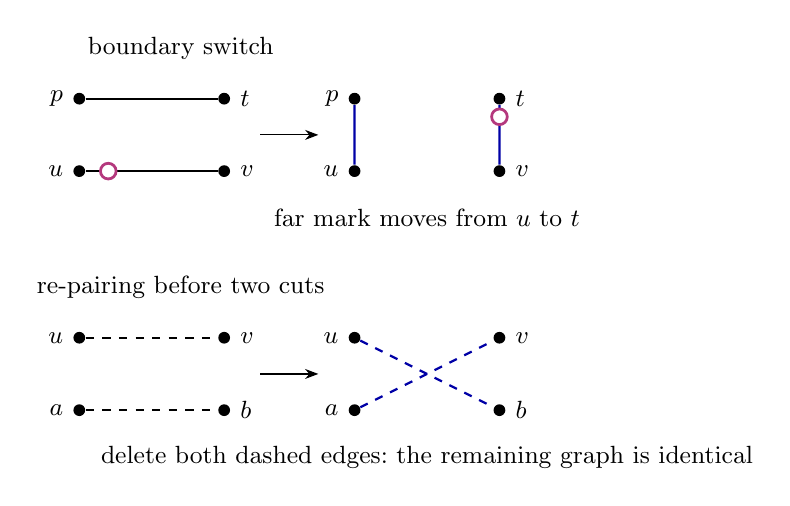
\begin{tikzpicture}[scale=.92,vertex/.style={circle,fill,inner sep=1.5pt},
                    every node/.style={font=\small},>=Stealth]
 \node at (1.4,1.7) {boundary switch};
 \node[vertex,label=left:$p$] (p1) at (0,1) {};
 \node[vertex,label=right:$t$] (t1) at (2,1) {};
 \node[vertex,label=left:$u$] (u1) at (0,0) {};
 \node[vertex,label=right:$v$] (v1) at (2,0) {};
 \draw[thick] (p1)--(t1) (u1)--(v1);
 \node[circle,draw=magenta!70!black,fill=white,line width=1pt,
       inner sep=2pt] at (.4,0) {};
 \draw[->] (2.5,.5)--(3.3,.5);
 \node[vertex,label=left:$p$] (p2) at (3.8,1) {};
 \node[vertex,label=right:$t$] (t2) at (5.8,1) {};
 \node[vertex,label=left:$u$] (u2) at (3.8,0) {};
 \node[vertex,label=right:$v$] (v2) at (5.8,0) {};
 \draw[thick,blue!65!black] (p2)--(u2) (t2)--(v2);
 \node[circle,draw=magenta!70!black,fill=white,line width=1pt,
       inner sep=2pt] at (5.8,.75) {};
 \node[align=center] at (4.8,-.65) {far mark moves\ from $u$ to $t$};
 \begin{scope}[yshift=-3.3cm]
 \node at (1.4,1.7) {re-pairing before two cuts};
 \node[vertex,label=left:$u$] (u3) at (0,1) {};
 \node[vertex,label=right:$v$] (v3) at (2,1) {};
 \node[vertex,label=left:$a$] (a3) at (0,0) {};
 \node[vertex,label=right:$b$] (b3) at (2,0) {};
 \draw[thick,dashed] (u3)--(v3) (a3)--(b3);
 \draw[->] (2.5,.5)--(3.3,.5);
 \node[vertex,label=left:$u$] (u4) at (3.8,1) {};
 \node[vertex,label=right:$v$] (v4) at (5.8,1) {};
 \node[vertex,label=left:$a$] (a4) at (3.8,0) {};
 \node[vertex,label=right:$b$] (b4) at (5.8,0) {};
 \draw[thick,dashed,blue!65!black] (u4)--(b4) (a4)--(v4);
 \node[align=center] at (4.8,-.65) {delete both dashed edges:\ the remaining graph is identical};
 \end{scope}
\end{tikzpicture}
\caption{The upper switch attaches a sampled cavity at $u$ to the
internal vertex $p$, retaining a reversible stub mark.  The open circles
mark the selected outgoing stubs at $u$ before the switch and $t$ after it.
The lower re-pairing is used only to estimate Green entries between the two
endpoints of a cut edge.  After both displayed edges are removed the
graph is unchanged, while $u$ and $v$ belong to different sampled edge
groups.  The drawings specify stub pairings; they assert no independence
of neighboring Green functions.}
\label{fig:local-switch}
\end{figure}

Apply the switch only when the internal exploration has no collisions,
the required parent and pending stub data are distinct except for shared
internal vertices, the far pairs have distinct data disjoint from the
explored data, all replacements are simple, and the inverse instructions
are applicable and restore the input.  On the complementary set define
the transformation to be the identity.  This definition makes it an
involution of the marked sample space.  Its nontrivial part preserves
weights: the underlying matching, each base mark, each far outgoing
stub, and each ordering seed have the same weight before and after the
operation.  A bounded collection of initially separated tree
neighborhoods satisfies all the requirements.  In such neighborhoods no
new edge duplicates an old edge, and reversal reads the same pending
positions and distinct far data.  Consequently the excluded set has
probability $O(n^{-1})$.

This also applies to two independently sampled bases, whose internal
trees are disjoint outside an $O(n^{-1})$ event.  The two observations
use one common switched graph; a cavity observation deletes only its
own marked base edge from that graph, not the other observation's edge.  We do not require
additional acyclicity among exterior vertices as a condition of
reversal.  Thus bounded switch averages may ignore failures at cost
$O(n^{-1})$ and otherwise use the original joint law of the graph and
its marks.  Potentials are attached to vertices and are never used in
choosing a switch, so their iid law is preserved.

\paragraph{Resolvent comparison after switching.}
For the next argument, say that a scalar or fixed-dimensional matrix
error is small if it has norm at most $y^{-a}$ outside an event of
probability at most $Cy^{-a}$, for some $a>0$.  There are only boundedly
many entries and operations, with bounds depending on $j,d$.
Lemma~\ref{lem:spectral-averaging} permits multiplication of a small
error by every fixed number of Green entries that occurs below.
Indeed, if the original exponent is $a$ and at most $N$ factors occur,
restrict each factor to at most $y^\epsilon$ with
$\epsilon<a/(2N)$.  The product still has a negative-power bound, and
the union of tail exceptions has a negative-power probability.
Also $n^{-a}$ is small in this sense since $y\le hn$.

Partition the selected coordinates according to their independent
samplings: one group for each base and its internal vertices, original
boundary endpoints, and designated parent if present; one group for
each far pair.  Lemma~\ref{lem:ward} and Markov's inequality show that
in the unmodified Green matrix all entries joining different groups
are small.  First sever every pending edge and every far edge, and
also sever the base edge for a cavity observation.  We claim that the
cross-group entries stay small and that each far-pair block stays close
to its block with only its own edge deleted.

Here is the finite-rank calculation behind this claim.  Suppose a
bounded update $B$ is supported in a single group $S$, let
$Q=G_{SS}$, and let $Q'=G'_{SS}$ be its updated compression.  The
identities
\begin{equation}\label{eq:group-update}
 \begin{split}
 (I+BQ)^{-1}&=I-BQ',\\
 G'_{UW}-G_{UW}&=-G_{US}(I+BQ)^{-1}B G_{SW}
 \end{split}
\end{equation}
hold for any two coordinate sets $U,W$.  Both $Q$ and $Q'$ have the
bounds allowed above, since the updates and coordinate choices are
independent of the potentials.  If $U$ and $W$ are distinct groups,
at least one factor crossing to $S$ is small; if both belong to a
different group, both crossing factors are small.  Formula
\eqref{eq:group-update} also applies when one of $U,W$ is $S$.
Severing one group at a time proves the claim.  To compare a given
far block with its individual single-cut block, perform that group's
cut first.

We still need smallness between the two ends of a severed far edge.
This does not follow from the Ward estimate for independent locations,
since the endpoints of an uncut edge were sampled together.  Introduce
another independently sampled far pair, if one is not already available,
and write the two pairs as $(u,v)$ and $(a,b)$.  Re-pair them as
$(u,b)$ and $(a,v)$, and then sever both pairs.  The resulting double-cut
graph is exactly the same as when $(u,v)$ and $(a,b)$ were severed.
The re-pairing is an equal-weight marked switch with $O(n^{-1})$
failure probability, by the preceding construction.  In its new marked
representation, $u$ and $v$ belong to different edge groups.  The
cross-group estimate already proved therefore makes their entry in
the double-cut graph small.  If the second pair was introduced solely
for this argument, restore its original edge: the cross entries
between the original groups $\{u,v\}$ and $\{a,b\}$ are small, so \eqref{eq:group-update} preserves the
conclusion.  This proves the required estimate without any assumption
about a cut edge's two endpoints.

At this point the internal tree to be observed is isolated.  Restore
all exterior replacement edges $t-v$, postponing attachment of this
internal tree until the end.  For two bases, also perform the other
base's updates; its parent edge is restored to its ordinary uncut
status because the present cavity observation deletes only its own
base edge from the common switched graph.  Every cross entry from a new
leaf $u$ to these update coordinates is small, including the entry
to its former partner $v$ just treated by re-pairing.  Here take $S$ to be exactly the coordinates changed in this exterior
step: the relevant $t$'s and $v$'s and, when present, the other base's
update coordinates.  This set excludes the present input leaves and
need not be a union of original groups.  Formula
\eqref{eq:group-update} applies to this support as well: every entry
from a present leaf to $S$ is small, and the inverse factor on $S$
still has the fixed-dimensional compression bound.  Therefore the
boundary Green matrix on the new leaves differs by a small error from
the diagonal matrix whose entries are
\[
             G^{[uv]}_{uu}(\zeta)
\]
in the original graph with the individual far edge deleted.

Finally add the $p-u$ edges.  On the internal tree the exact Schur
matrix uses this boundary compression.  The inverse of that Schur
matrix is the internal compression of the final graph resolvent,
so its norm is at most any fixed small positive power of $y$ outside
a negative-power exception, by Lemma~\ref{lem:spectral-averaging}.
Replacing the boundary matrix by its diagonal approximation changes
the Schur matrix by a small error.  The inverse identity, or its
Neumann expansion once the product of inverse norm and error is less
than $1/2$, shows that its inverse changes by a small error as well.
With the diagonal substitution, successive leaf elimination is exactly
the recursion $F_j$, or its full-root version, with the original internal
potentials.  The map $X$ has bounded derivative on $\HH$, uniformly
for $e\in J$, and so conversion to disk coordinates preserves the
error estimate.  This establishes the claimed recursion comparison
for each of one or two switched observations on the same switched data.

\paragraph{Replacing empirical internal potentials by iid potentials.}
The preceding comparison still uses potentials at an empirically
sampled base.  We next replace their empirical law by the deterministic
iid law while keeping independence from the sampled cavity inputs.
Let $k_j$ be the number of internal vertices.  Bin each potential
coordinate on a mesh $n^{-\alpha}$, with $\alpha>0$ sufficiently small
for this fixed $k_j$.  Let $\mu_H$ be the empirical law of the internal
potential vector, including the ordering randomness and a default on
tree failures, and let $\mu$ be the iid potential law.
For each product bin $B$, one- and two-base explorations give
\[
 |\EE\mu_H(B)-\mu(B)|=O(n^{-1}),\qquad
 |\EE\mu_H(B)^2-\mu(B)^2|=O(n^{-1}).
\]
Indeed disjoint valid neighborhoods have independent potential vectors,
and all failures cost $O(n^{-1})$.  Hence
$\EE|\mu_H(B)-\mu(B)|=O(n^{-1/2})$.
There are $O(n^{\alpha k_j})$ bins, so choosing
$\alpha k_j<1/4$, for example, bounds the expected total variation
of the binned laws by a negative power of $n$.

Couple the bins maximally and, on a matched bin, fill in an iid vector
with its conditional distribution inside that bin.  Thus internal
potential vectors can be coupled with coordinate error $O(n^{-\alpha})$
outside an event of negative-power probability.  Given $H$, this
coupling uses only the base sampling and additional randomness.  It
is consequently independent of all far-edge samples, which give iid
single-cut values with law $P_H$ conditional on $H$.  For two bases
use independent such couplings conditional on $H$; their target
potential vectors are iid and independent of both collections of
inputs.  Dependence of $P_H$ on the potentials creates no difficulty
in this conditional assertion.

Changing the finitely many internal potentials by the coupled error
changes the finite-tree recursion by a small error.  This follows
from the same Schur inverse perturbation just used.  Alternatively,
with iid internal potentials the effective finite-tree inverse
satisfies the final assertion of Lemma~\ref{lem:spectral-averaging},
uniformly in its dissipative leaf data.  The comparison also records
the internal potential coordinates themselves, which proves the
augmented version of the approximation.

We have thus constructed the coupling announced above.  For one or
two bases, $\widehat O_i$ is the observation at base $i$ in the common
switched graph, and $R_i$ is the recursion output formed from its
original far-edge samples and the coupled iid internal potentials.
The bounded test $f$ turns the comparison errors into
\begin{equation}\label{eq:switched-observation-comparison}
 \EE|f(\widehat O_i)-f(R_i)|\le Cy^{-c}.
\end{equation}
Conditional on $H$, the $R_i$ are independent and
$\EE[f(R_i)\mid H]=d_H$.  Marked-switch invariance preserves the
joint law of $\widehat H$ and its sampled observations
$\widehat O_i$, while their comparison partners $R_i$ use the original $H$.

\paragraph{Stability of the recursion prediction under a switch.}
For the mixed-moment comparison, we need
\begin{equation}\label{eq:multiplier-stability}
                       \EE|d_{\widehat H}-d_H|\le Cy^{-c}.
\end{equation}
To prove it, use fresh independent far-edge samples for the inputs
defining $d_H$.  Couple the samples in $H$ and $\widehat H$ by their
outgoing stubs; they agree away from the bounded set of modified stubs,
and overlap with update data has probability $O(n^{-1})$.
The old Green entries between each fresh sample group and the update
groups are small by Lemma~\ref{lem:ward}.  Sever its own edge first
and apply \eqref{eq:group-update} through the remaining cuts and
updates, using the union of their coordinates as the support $S$
when an update joins different original groups.  These cross entries stay small, and its single-cut diagonal
changes by a small error, in half-plane as well as disk coordinates.
Use the same fresh iid internal potentials for the two predictions.
The dissipative finite-tree compression bound in
Lemma~\ref{lem:spectral-averaging} and inverse perturbation compare
the two outputs.  Boundedness of $f$ turns the exceptional probabilities
and the good-event errors into \eqref{eq:multiplier-stability}.

\paragraph{Two observations and transportation distance.}
We can now complete the proof of Proposition~\ref{prop:empirical-recursion}.
With two bases, switch invariance and conditional independence give
\[
 \EE[f(\widehat O_1)f(\widehat O_2)]=\EE a_H^2,
 \qquad
 \EE[f(R_1)f(R_2)]=\EE d_H^2.
\]
The coupling bound \eqref{eq:switched-observation-comparison} and
$|f|\le1$ therefore imply
$|\EE a_H^2-\EE d_H^2|\le Cy^{-c}$.
With one base, switch invariance gives
$\EE[f(\widehat O_1)d_{\widehat H}]=\EE(a_Hd_H)$.
Replacing the multiplier by $d_H$ costs $Cy^{-c}$ by
\eqref{eq:multiplier-stability}; replacing $f(\widehat O_1)$ by
$f(R_1)$ costs the same by
\eqref{eq:switched-observation-comparison}.  Finally,
$\EE[f(R_1)d_H]=\EE d_H^2$, by conditioning on $H$.  Thus
\[
                   |\EE(a_Hd_H)-\EE d_H^2|\le Cy^{-c}.
\]
Combining these two comparisons yields
\begin{equation}\label{eq:empirical-test-variance}
                         \EE|a_H-d_H|^2\le Cy^{-c}.
\end{equation}
In particular the comparison is within each random empirical law,
not just after ensemble averaging.

For completeness, pass from tests to transportation as follows.
Embed the compact coordinate space in a fixed Euclidean cube and
use a tent partition of unity on a mesh $\delta=y^{-\epsilon}$.
There are $O(\delta^{-k})$ functions for a fixed dimension $k$, each
bounded by one and with Lipschitz constant $O(\delta^{-1})$.
Applying \eqref{eq:empirical-test-variance} to rescaled functions
bounds the expected sum of their mass discrepancies by
$C\delta^{-k-1}y^{-c/2}$.  Match the common mass in each tent and
couple the unmatched mass arbitrarily.  Since each tent has diameter
$O(\delta)$ and the whole space has bounded diameter, the resulting
squared transportation cost is at most a constant times $\delta^2$
plus that sum of discrepancies.  Choose $\epsilon$ small and apply
Markov's inequality.  This gives \eqref{eq:empirical-recursion}, with
a smaller positive exponent, for the cavity, full-root, and augmented
laws.  The proof of Proposition~\ref{prop:empirical-recursion} is complete.

\subsection{Descending the imaginary part}

The empirical recursion now supplies the hypotheses of the tree
stability theorem, except for its smallness condition.  We establish
that condition at a fixed positive height and retain it while descending.

\begin{proof}[Proof of Proposition~\ref{prop:local-law}]
At $\eta=h$, the cavity resolvent at a vertex with a sufficiently large
fixed tree neighborhood is close to the clean-tree cavity value,
first by polynomial approximation of the resolvent and then by the
norm perturbation bound $Cw/h^2$.  Equivalently one may approximate
the disordered resolvent locally and use its bounded potential
perturbation.  The polynomial degree is fixed after $h$ and the desired
accuracy are chosen; the Hamiltonians have uniformly bounded spectra.
The fraction of vertices failing this fixed tree test has expectation
$O(n^{-1})$.  Write $\delta_*$ for the fixed $L^2$ smallness threshold in
Proposition~\ref{prop:tree-stability}.  As permitted by its parameter
order, take $h$ small and then $w_0/h^2$ small enough that the starting
disk norm is below $\delta_*/2$, and take the target tree norm below
$\delta_*/4$.  Polynomial approximation with a sufficiently small
fixed error then places $P_H$ inside the threshold with failure
probability $O(n^{-1})$.

Fix $r\in(0,1)$ sufficiently close to one.  For any diagonal Green
function of a fixed graph or cut graph, Schwarz--Pick applied to its
map from $\HH$ to $\DD$ implies a uniform bound on its change between
$e+i\eta$ and $e+ir\eta$ tending to zero as $r\uparrow1$.
Choose $r$ so that this change is smaller than the gap between the
improved smallness bound and the threshold.  Starting at $h$, descend
through $h,rh,r^2h,\ldots$, shortening the last step to reach the
prescribed $\eta$.  At each height apply
Proposition~\ref{prop:empirical-recursion} for $j=1,\ell$ and then
Proposition~\ref{prop:tree-stability}.  Its conclusion places $P_H$
within $C(n\eta)^{-c}$ of $Q_\zeta$, hence back well inside the
threshold when $y_0$ is large.  This closes the induction.

The failure probabilities sum geometrically from the smallest height:
if $\eta_*$ is the terminal height, then
\[
             \sum_{\text{heights }\eta_k\ge\eta_*}
                       C(n\eta_k)^{-c}\le C'(n\eta_*)^{-c}.
\]
The initial $O(n^{-1})$ failure fits this bound after decreasing $c$.
We obtain \eqref{eq:distributional-local-law} for $P_H$.
For the full-root law, use the full-root version of
Proposition~\ref{prop:empirical-recursion} with one internal level.
Couple the cavity inputs to iid tree inputs optimally and apply the
sibling estimate \eqref{eq:tree-sibling-bound}, with $d$ children.
Its coefficients involve inverse margins of the other tree inputs,
whose required fixed moments are bounded.  Independence of the coupled
input pairs therefore bounds the output $L^2$ error by a constant
times the input $W_2$ error.  This proves the full statement.
\end{proof}

\subsection{Environment, trace, and microscopic integrability}

The disk metric was convenient for stability because it is bounded.
For later spectral and eigenvector arguments we need consequences in
half-plane coordinates, where large values must be controlled.  The
intercept $B_v$ in \eqref{eq:intercept} provides that control because
it is independent of the potential at the observed site.

\begin{corollary}[Consequences of the local law]
\label{cor:local-consequences}
Fix $E$ in the interior of $J$ and $s\in\RR$.  The following statements
hold.
\begin{enumerate}
\item At $\zeta=E+(s+iy)/n$, in the order $n\to\infty$ and then
$y\to\infty$, the diagonal $G_{vv}(\zeta)$ at a uniform vertex,
jointly with every fixed ordered neighborhood of potentials around
$v$, converges to the tree diagonal $m_o(E+i0)$ with the corresponding
tree environment.  For any fixed number of independently sampled
vertices the joint assertion holds with independent tree environments,
and their off-diagonal Green entries tend to zero in probability.
The diagonal assertion also holds along every sequence
$n\eta\to\infty$, $(e,\eta)\to(E,0)$.
\item There are $c,C>0$ such that, for every sufficiently large fixed $y$,
\begin{equation}\label{eq:trace-slow-power}
 \limsup_{n\to\infty}\PP\left\{
 \left|\Im\frac1n\Tr G\left(E+\frac{s+iy}{n}\right)
             -\pi\rho_{d,w}(E)\right|>y^{-c}\right\}\le Cy^{-c}.
\end{equation}
The constants are independent of the fixed real number $s$.
\item For each fixed $s\in\RR$ and $y>0$, the sampled diagonal imaginary
parts are uniformly integrable in the following limiting sense:
\begin{equation}\label{eq:microscopic-ui}
 \lim_{T\to\infty}\limsup_{n\to\infty}
 \EE_{H,v}\left[
 \Im G_{vv}\left(E+\frac{s+iy}{n}\right)
 \mathbf1_{\{\Im G_{vv}(E+(s+iy)/n)>T\}}\right]=0.
\end{equation}
\end{enumerate}
The double-limit assertion in the first item means that, for bounded
continuous tests, the limsup of the discrepancy as $n\to\infty$
tends to zero as $y\to\infty$.
\end{corollary}

\begin{proof}
For the first item, take the augmented recursion of
Proposition~\ref{prop:empirical-recursion} with internal levels covering
the prescribed neighborhood.  By Proposition~\ref{prop:local-law},
its input law tends to the tree cavity law.  Its internal iid potential
coordinates are independent of these inputs by construction.
The tree recursion with these data is exactly the joint tree law of
the diagonal and the observed neighborhood.  For any fixed additional
depth this passage only needs weak convergence: all limiting input
values lie in the open disk almost surely, where the finite recursion
is continuous.  Thus no higher inverse-margin order is required as the
observed radius grows.  Proposition~\ref{prop:tree-stability} supplies
the common-environment boundary continuity.  Conversion back to the
half-plane is valid since the limiting tree value is finite almost
surely.  The empirical-law conclusion gives product limits for
independently sampled vertices, and their mutual Green entries vanish
by \eqref{eq:sampled-ward}.  These arguments apply along every parameter
sequence stated in the corollary.  A diagonal choice of sequences gives
the stated double-limit formulation.  Letting the finite radius
increase identifies the limit with the measurable function
$m_o(E+i0)$ of its complete tree environment.

We next obtain a useful quantitative bound on small intercepts.
For a half-plane value $g$ and $x=X(g)$, the comparison used in
\eqref{eq:tree-hyperbolic-comparison} gives
\[
 \frac{\Im g}{|g|^2}\ge c_J(1-|x|).
\]
Couple $P_H^0$ with the tree law using
\eqref{eq:distributional-local-law}.  The bounded diameter of the disk
also bounds the expectation of its squared transportation error by
a negative power of $y$.  Markov's inequality for this coupling and
the tree inverse-margin moments show, for a sufficiently small
$\epsilon>0$, that
\begin{equation}\label{eq:small-intercept-large-height}
 \PP_{H,v}\{B_v(\zeta)<y^{-\epsilon}\}\le Cy^{-c}.
\end{equation}
For example, if the tree disk margin is at least $2\delta$ and the
coupling distance is below $\delta$, the finite margin is at least
$\delta$; take $\delta$ to be a sufficiently small power of $y^{-1}$.
This proves the bound directly from the two respective tail estimates.

The intercept formula gives $\Im G_{vv}\le B_v^{-1}$.
Since $B_v$ is independent of $V_v$, conditional spectral averaging
implies, for every $T>0$,
\begin{equation}\label{eq:intercept-tail-mean}
 \EE\bigl[\Im G_{vv}\mathbf1_{\{\Im G_{vv}>T\}}\bigr]
 \le \EE\bigl[\Im G_{vv}\mathbf1_{\{B_v<T^{-1}\}}\bigr]
 \le C_w\PP\{B_v<T^{-1}\}.
\end{equation}
This estimate applies after averaging over the uniform vertex as well.
Thus truncating the imaginary part at $T=y^\epsilon$ loses only a
negative-power amount in expectation, by
\eqref{eq:small-intercept-large-height}.  Tree tails have the same
property by their moment bounds.

To compare truncated imaginary parts through the disk local law,
first introduce a disk cutoff with margin $y^{-\epsilon'}$.
On the remaining compact subdisk, the function $x\mapsto\Im X^{-1}(x)$
has a Lipschitz constant bounded by a fixed power of $y^{\epsilon'}$.
Choose $\epsilon'$ small enough for the transportation estimate to
absorb this factor.  The mass removed by the cutoff has a negative-power
bound by the same coupling argument.  Choose the clipping exponent
$\epsilon$ still smaller, so that multiplying this mass by $y^\epsilon$
retains a negative-power bound.  Combining the comparisons and then
using Markov's inequality gives a negative-power bound for the
difference between the empirical imaginary trace and
$\EE\Im m_o(e+i\eta)$.  In the microscopic substitution with fixed
$s,y$, continuity of the tree expectation gives
$\EE\Im m_o\to\pi\rho_{d,w}(E)$ by
Corollary~\ref{cor:tree-density}.  This proves
\eqref{eq:trace-slow-power}, after decreasing $c$.  All finite-graph
constants were uniform in $e\in J$, hence are independent of fixed $s$.

Finally fix a possibly small microscopic height $y>0$.
The quantity $B_v(\zeta)$ is the imaginary part of the Herglotz function
\[
 \zeta+\langle a_v,(H^{(v)}-\zeta)^{-1}a_v\rangle,
\]
where $H^{(v)}$ deletes the vertex and $a_v$ is its adjacency column.
For $Y\ge y$, Harnack's inequality at the same real part yields
\[
 B_v\left(E+\frac{s+iy}{n}\right)
 \ge\frac yY B_v\left(E+\frac{s+iY}{n}\right).
\]
Choose a sufficiently large fixed $Y$.  Once
$\delta<(y/Y)Y^{-\epsilon}$, the probability that the left intercept
is below $\delta$ is at most the small-intercept probability at height
$Y$.  Consequently
\[
 \lim_{\delta\downarrow0}\limsup_n
 \PP\left\{B_v\left(E+\frac{s+iy}{n}\right)<\delta\right\}
 \le CY^{-c}.
\]
Let $Y\to\infty$ and apply \eqref{eq:intercept-tail-mean} to obtain
\eqref{eq:microscopic-ui}.  This last conclusion will retain the
normalization of eigenvector marks when taking microscopic limits.
\end{proof}

\section{Empirical eigenvector laws and conditional entropy}\label{sec:entropy}

Fix \(E\in I_{d,\kappa}\), and abbreviate
\(\rho=\rho_{d,w}(E)>0\).  The local law describes the environment seen
by a typical vertex.  We now retain eigenvector coordinates at that
vertex as well.  The objective of this section is an entropy inequality
for their law conditional on the entire potential environment.  In
Section~\ref{sec:rigidity}, equality in a complementary entropy bound
will identify this conditional law as Gaussian.

Choose a measurable real orthogonal eigenbasis \(u_1,\ldots,u_n\),
ordered by eigenvalue and normalized by
\(\langle u_i,u_j\rangle=n\delta_{ij}\).  Write
\begin{equation}\label{eq:microscopic-positions}
 x_i=n(\lambda_i-E),\qquad \nu_n=\sum_{i=1}^n\delta_{x_i}.
\end{equation}
A finite list of eigenvectors gives each vertex an \(\RR^m\)-valued
mark, one coordinate for each member of the list.  We call these
coordinates colors.  All lists below are finite, but their length is
arbitrary and imposes no additional smallness condition on \(w\).

\subsection{Keeping the empirical law in the limit}

For a fixed finite list, sample a uniform vertex and read its marked
neighborhood.  On a tree neighborhood use a uniformly ordered rooted
tree isomorphism; outside it use the nonbacktracking lift, recording a
failure flag.  Conditional on the graph, potentials, and eigenvectors,
this procedure defines an empirical probability law.  It is important
to retain this law, rather than just its average: independent vertex
samples are independent conditional on the empirical law.

\begin{proposition}[Marked subsequential limits]\label{prop:marked-limits}
Every sequence of admissible sizes tending to infinity has a
subsequence on which \(\nu_n\) converges in law to a locally finite
point measure \(\nu\).  On a further subsequence one can retain jointly
the positions and the empirical marked-neighborhood laws for the
eigenvalue-ordered lists in an exhaustion by bounded intervals,
together with all their finite truncations and restrictions.
Repeated limiting positions retain separate marks.

Almost every resulting empirical law \(\mathcal L\), with \(m\) colors,
is an automorphism-invariant law on the \(d\)-regular tree, whose
potential marginal is the deterministic iid uniform law on
\([-w,w]\).  If \(U_v\in\RR^m\) is its mark at \(v\), then
\begin{equation}\label{eq:mark-normalization-equation}
 \EE_{\mathcal L}U_oU_o^{\mathsf T}=\Id_m,
 \qquad
 (V_v-E)U_v+\sum_{u\sim v}U_u=0\quad\text{at every }v.
\end{equation}
The empirical laws and their restrictions to smaller lists can be
chosen consistently.
\end{proposition}

\begin{proof}
The Wegner bound of Lemma~\ref{lem:spectral-averaging} gives tightness
of the point measures on each compact interval.  Choose interval
endpoints uncharged almost surely by a subsequential limit; such an
exhaustion exists, since the expected limiting counts are bounded by
the same constant times interval length.  Truncate each list length
and then stratify by that length.  At a uniformly sampled vertex the
sum of squared coordinates of a list of length \(m\) has mean \(m\).
This proves tightness of all finite-radius observations.  A diagonal
extraction retains all radii, list truncations, and interval
restrictions, as well as their positions.

For each fixed radius the fraction of vertices with a non-tree
neighborhood tends to zero.  Uniform rooted orderings give invariance
under root-preserving automorphisms.  Sampling an oriented edge and
reversing it gives invariance under re-rooting across an edge; together
these give full tree-automorphism invariance.  The empirical law of
the potential labels alone converges in probability to their iid
tree law: one and two sampled bounded neighborhoods have this law
asymptotically, and two disjoint neighborhoods use independent
potentials.  Thus this marginal is deterministic inside each
limiting \(\mathcal L\).

The second-moment assertion needs more than tightness.  If the list
comes from \([-L,L]\), spectral decomposition gives
\begin{equation}\label{eq:marks-dominated-by-resolvent}
 \sum_{i\text{ in list}}u_i(v)^2
 \le (1+L^2)\Im G_{vv}(E+i/n).
\end{equation}
The right side is uniformly integrable at a sampled vertex by
Corollary~\ref{cor:local-consequences}.  Consequently the limiting
empirical second moments lose no mass.  More explicitly, represent
the joint convergence almost surely, first pass bounded
second-moment truncations, and then remove the truncation using the
tail bound in expectation.  The empirical moments before taking the
limit are exactly \(\delta_{ij}\), so their limits are the same almost
surely; polarization handles the mixed moments.  The eigenvalue
equations pass to the limit on every finite neighborhood because
\(\lambda_i=E+O_L(n^{-1})\).  Countable consistency gives the assertions
simultaneously at all vertices and for all retained lists.
\end{proof}

We henceforth fix one such \(\mathcal L\) when making assertions about
a conditional law.  We write \(\omega=(V_v)_{v\in T_d}\) for its full
potential environment; thus \(\omega\) here records the coupled
potentials themselves.  Expectations with respect to its deterministic
iid marginal are denoted \(\EE_\omega\).

\subsection{Eliminating a conditional mean}

Orthogonality alone does not show that
\(\EE_{\mathcal L}[U_o\mid\omega]\) vanishes.  A coherent component
depending on the potential environment would survive it.  The
following perturbation averages such a component over a physical
energy interval longer than the microscopic window, while changing
the ensemble by a vanishing total variation distance.

\begin{lemma}[Conditional centering]\label{lem:conditional-mean}
For almost every empirical law in Proposition~\ref{prop:marked-limits},
\begin{equation}\label{eq:conditional-zero-mean}
 \EE_{\mathcal L}[U_v\mid\omega]=0
 \qquad\text{at every vertex }v.
\end{equation}
\end{lemma}

\begin{proof}
Let \(f\) be a bounded Lipschitz function of the potentials in a
fixed rooted ball.  Average over its branch orderings and put the
corresponding finite-graph value \(f(v)\) equal to zero at tree
failures.  First require that \(f\) vanish unless the central
potential belongs to a compact subinterval of \((-w,w)\).  Choose
\(b_0\in C_c^\infty((-w,w))\), nonnegative and bounded below by a
positive constant on that subinterval.  For
\(0\le t\le a_n:=n^{-2/3}\), change every potential by
\[
 V_v\longmapsto V_v+t b_0(V_v).
\]
For large \(n\) this is a diffeomorphism of \([-w,w]\), identical
near its endpoints.  The one-site density ratio is \(1+O(t)\), has
integral one, and has second moment \(1+O(t^2)\).  Independence
therefore bounds the total variation distance of the product laws by
\(O(\sqrt n\,t)=o(1)\), uniformly over this range.  The normalized
test vector \(f/\sqrt n\) changes by \(O_f(t)\) in Euclidean norm.

For the original configuration set
\(B=\diag(b_0(V_v))\).  The support condition writes
\(f/\sqrt n=B^{1/2}q_f\), with \(\|q_f\|\le C_f\).  Scalar spectral
averaging gives, for every interval \(I\),
\begin{equation}\label{eq:bump-spectral-averaging}
 \int_0^{a_n}
 \left\langle f/\sqrt n,\mathbf1_I(H+tB)f/\sqrt n\right\rangle\,dt
 \le C_f|I|.
\end{equation}
For completeness, compress the resolvent by Schur complement to the
indices where \(B>0\), and conjugate by \(B^{1/2}\).  It becomes
\((t\Id-T)^{-1}\) with \(\Im T>0\) at positive spectral height.
The integral of its imaginary part in a vector, over the real
\(t\)-axis, is at most \(\pi\) times that vector's squared norm.
The Herglotz representation, followed by spectral inversion, proves
\eqref{eq:bump-spectral-averaging}; restricting the nonnegative
integrand to \([0,a_n]\) preserves the bound.

Take \(I=E+[-L,L]/n\), divide by \(a_n\), and average over the
original data.  Total variation comparison and the change in the
test vector show that
\[
 \EE\left\langle f/\sqrt n,\mathbf1_I(H)f/\sqrt n\right\rangle
 \le O_f(n^{-1/3})+o(1).
\]
The left side is
\(\EE\sum_{x_i\in[-L,L]}(n^{-1}\sum_v f(v)u_i(v))^2\).
Hence every empirical root average against \(f\) vanishes in the
limit.  Passing these first moments is justified by the uniform
second-moment bounds.  A countable dense collection of tests on all
finite balls, followed by an exhaustion of \((-w,w)\) in the central
coordinate, determines the full conditional mean.  Averaging tests
over branch orderings loses no information, since the rooted joint
law is invariant under those permutations.  Re-rooting proves the
claim at every vertex.
\end{proof}

\subsection{Counting labels while retaining the environment}

We use natural logarithms, write \(H\) for discrete entropy, and
write \(\mathcal H\) for differential entropy.  Conditional
differential entropy means the integral of the entropy of the
conditional law.  Our entropy argument follows the colored-tree and
Gaussian-smoothing framework of Backhausz and Szegedy
\cite[Theorems~6.1 and 8.1]{BackhauszSzegedy2019}.  The extra issue is
that the conditioning environments attached to adjacent vertices
overlap.  We keep these labels in the count, and later compute their
entropy contribution explicitly.

Fix a radius \(R\ge0\) and divide \([-w,w]\) into \(Q\) equal
intervals.  The environment label at a vertex records the rooted
isomorphism type of its radius-\(R\) neighborhood with these binned
potentials, including its central bin.  Adjoin a label from any
fixed finite alphabet for its mark.  Tree failures may use a separate
label, which still records the central potential bin.  The resulting
alphabet has fixed finite size \(M\).
For any vertex labeling let \(T\) be its ordered star histogram,
symmetrized over neighbor permutations, and let \(S\) be its
oriented-edge histogram.

With probability tending to one over the graph and potentials,
simultaneously for all such histograms, the number of labelings
whose prescribed central bins are correct is at most
\begin{equation}\label{eq:environment-type-count}
 \exp\left\{n\left[H(T)-\frac d2H(S)-\log Q+o(1)\right]\right\}.
\end{equation}
The requirement that an entire environment label be correct can only
decrease this number.  Here is the first-moment count, including the
normalization of the potential term.  In the configuration model,
prescribe each vertex label and the labels desired at its ordered
half-edges.  If \(m_{ab}=ndS(a,b)\), the probability of a compatible
matching is
\[
 \frac{\prod_{a<b}m_{ab}!\,\prod_a(m_{aa}-1)!!}{(nd-1)!!},
\]
and is zero unless \(m_{ab}=m_{ba}\) and all \(m_{aa}\) are even.
Its logarithm is \(-ndH(S)/2+O_M(\log n)\).  The arrays of each
ordered star type \(T_0\) number at most \(\exp(nH(T_0))\), with
\(H(T_0)\le H(T)\).  There are only polynomially many types for
fixed \(M\).  Independently, the prescribed central bins agree with
the iid potentials with probability exactly \(Q^{-n}\).
Stirling's formula, Markov's inequality with a sublinear exponential
allowance, and a union bound prove \eqref{eq:environment-type-count}.
Conditioning on simplicity changes the estimates by a bounded factor.
This is the fixed-alphabet form of the count in
\cite[Section~3.1, Lemma~3.2]{bu}; its argument is independent of the
eigenvectors and remains valid with the added labels.

\subsection{From the count to full conditional entropy}

Fix \(\eta>0\) before taking the graph-size limit.  Add to the mark
array a centered Gaussian field, with independent colors and
covariance in each color
\begin{equation}\label{eq:entropy-smoothing}
 \Gamma_\eta=\Im(H-E-i\eta)^{-1}
     =\frac{\eta}{(H-E)^2+\eta^2}.
\end{equation}
Let \(F^\eta\) be the limiting sum of marks and noise.  At this fixed
height polynomial approximation on the uniformly bounded spectra
identifies the local noise covariance with the infinite-tree
covariance \(\Im(H_{T_d}-E-i\eta)^{-1}\).  Given \(\omega\), the
noise is independent of the marks.  Fix neighbor indices
\(1,\ldots,d\) on the rooted tree used for \(\mathcal L\).  A star
observation consists of the root followed by these neighbors; an
edge observation consists of the root and neighbor \(1\).  Their
ordering is inherited from the uniformly ordered finite lift,
and is the same ordering used in \(\omega\).

\begin{proposition}[Entropy conditional on the tree environment]
\label{prop:conditional-entropy}
For almost every empirical law \(\mathcal L\) with \(m\ge1\) colors,
and for every fixed height in any prescribed countable set of
positive heights,
\begin{equation}\label{eq:conditional-star-edge-entropy}
 \begin{split}
 &\mathcal H(F^\eta_{\rm star}\mid\omega)
       -\frac d2\mathcal H(F^\eta_{\rm edge}\mid\omega)\\
 &\hspace{1cm}\ge
 m\left[\frac12\log(2\pi\mathrm e\,\eta)
       -\int\log|t-E-i\eta|\,d\nu_{d,w}(t)\right].
 \end{split}
\end{equation}
\end{proposition}

\begin{proof}
For fixed environment radius \(R\) and number of bins \(Q\), let
\(A_{R,Q}\) and \(B_{R,Q}\) be the tuples of environment labels
seen by the ordered star and edge, respectively.  The count first gives
an inequality with these finite conditioning data:
\begin{align}
 &m\left[\frac12\log(2\pi\mathrm e\,\eta)
        -\int\log|t-E-i\eta|\,d\nu_{d,w}(t)\right]\notag\\
 &\quad\le
 \mathcal H(F^\eta_{\rm star}\mid A_{R,Q})
 -\frac d2\mathcal H(F^\eta_{\rm edge}\mid B_{R,Q})
 +H(A_{R,Q})-\frac d2H(B_{R,Q})-\log Q.
 \label{eq:finite-environment-entropy}
\end{align}
We shall derive this inequality by removing the mark bins at fixed
\(R,Q\).  The remaining environment contribution is
\begin{equation}\label{eq:environment-entropy-remainder}
 H(A_{R,Q})-\frac d2H(B_{R,Q})-\log Q.
\end{equation}
Its limit is zero as \(Q\to\infty\) at fixed \(R\); after that
cancellation, increasing \(R\) gives conditioning on \(\omega\).

We first keep the environment radius, its bins, and the noisy-mark
bins fixed.  Conditional on the finite graph, potentials, and list,
only the Gaussian noise is random.  The entropy of its binned
labeling is at most the entropy of its histogram type plus the
logarithm of the number of labelings of that type.  The first term
is \(O(\log n)\).  Using \eqref{eq:environment-type-count} for the
second term therefore bounds the entropy per vertex by
\[
 \EE_{\rm noise}H(T)-\frac d2\EE_{\rm noise}H(S)-\log Q+o(1).
\]
We may replace the random histograms by their conditional means in
this expression.  Indeed their individual cell frequencies have
variance tending to zero.  To see this, \(\Tr\Gamma_\eta^2=O_\eta(n)\)
implies that the average squared cross-covariance between two
independently sampled bounded local blocks is \(o(1)\).  Their
marginal covariances have deterministic upper and positive lower
bounds at fixed \(\eta\).  Gaussian continuity consequently makes
the average total variation distance to the product of the two
marginals tend to zero.  This remains true after arbitrary shifts
by the fixed eigenvectors and after binning.  Overlapping blocks
have vanishing probability.  Thus all histogram entropies converge
to those of the corresponding limiting observations.  Gaussian
smoothing removes mark-bin boundary atoms, and the potential bins
have null boundaries as well.

We next remove the mark binning, while retaining the finite
environment labels.  Use cubes of side \(\Delta\) in \(\RR^m\),
clipped outside a large box.  Before clipping, the entropy of the
global quantization is at least the global Gaussian differential
entropy minus \(nm\log\Delta\): the entropy within any cube is at
most its log volume.  Clipping changes the entropy per vertex by
an amount tending to zero with the box size, at fixed \(\Delta\).
For this last assertion it suffices to bound the average second
moment, which is bounded by normalization of the marks and the
fixed-height Gaussian covariance bound.  For example, compare the
tail-bin distribution with summable lattice weights proportional
to \((1+|j|)^{-C}\); its entropy is bounded by its tail probability
times a logarithmic moment bound.  The same argument applies to
each finite-dimensional limiting observation.

After removing the clipping, send \(\Delta\downarrow0\).  The
smoothed densities are bounded and continuous, and have finite
second moments.  Replacing a density by its uniform filling in
each bin gives \(L^1\) convergence; the density bound and the
preceding tail estimate give entropy convergence.  The log-volume
terms cancel because
\(m(d+1)-(d/2)(2m)=m\).  The lower bound furnished by the full
Gaussian array is
\begin{align*}
 \frac1n\mathcal H(\text{global Gaussian noise})
 &=\frac m2\log(2\pi\mathrm e)
       +\frac m{2n}\log\det\Gamma_\eta\\
 &=m\left[\frac12\log(2\pi\mathrm e\,\eta)
       -\frac1n\sum_{i=1}^n\log|\lambda_i-E-i\eta|\right].
\end{align*}
The empirical spectral measure converges to \(\nu_{d,w}\), by
polynomial approximation and convergence of bounded-neighborhood
observations.  Splitting each limiting joint entropy into the entropy of its
environment labels and its conditional mark entropy gives
\eqref{eq:finite-environment-entropy}.

We now compute the environment contribution
\eqref{eq:environment-entropy-remainder} before increasing the radius.  Set
\[
 s_R=\sum_{k=0}^{R}b^k,\qquad p_R=\sum_{k=0}^{R-1}b^k,
 \qquad p_0=0.
\]
The star's collection of labels reads \(1+ds_R\) potential bins:
the ball of radius \(R+1\), with its first neighbor positions
ordered and its remaining branches unordered.  The edge reads
\(2s_R\) bins in its two outward half-balls.  When all these bins
are distinct the overlaps identify the vertices uniquely.  There
are \(dp_R\) independent outward permutations of \(b\) branches
in the star reading and \(2p_R\) in the edge reading.  Thus
\begin{align*}
 H(A_{R,Q})&=(1+ds_R)\log Q-dp_R\log(b!)+o_Q(1),\\
 H(B_{R,Q})&=2s_R\log Q-2p_R\log(b!)+o_Q(1).
\end{align*}
For fixed \(R\), bin collisions have probability \(O_R(Q^{-1})\);
their entropy cost is \(O_R(Q^{-1}\log Q)\), which justifies the
errors.  Both the bin counts and the permutation losses cancel in
\eqref{eq:environment-entropy-remainder}, leaving \(o_Q(1)\).

Take nested potential partitions as \(Q\to\infty\).  Almost surely
all finitely many potentials in a reading are distinct, so its
limiting information is exactly the corresponding continuous
potential configuration modulo the indicated permutations.
Conditioning instead on fully ordered potentials in that union
does not change the observation entropy: each omitted permutation
fixes the observed star or edge, and invariance of \(\mathcal L\)
makes its conditional observation law identical under that
permutation.  Finally let \(R\to\infty\); these ordered
configurations exhaust \(\omega\).

Here the conditioning limits can be justified without subtracting
infinite entropies of continuous environments.  Use relative
entropy with respect to a fixed product Gaussian reference on
the observation coordinates and apply monotone convergence on
the increasing conditioning sigma-fields.  The conditional
relative entropy is finite: fixed-height smoothing bounds
conditional entropy below by noise entropy, while second moments
bound it above.  This proves convergence of the conditional
entropies and hence \eqref{eq:conditional-star-edge-entropy}.

All passages have been made for fixed finite choices before
refinement.  To make them hold inside almost every empirical law,
include the countably many bin choices and heights in the joint
subsequence construction, and take a further subsequence on which
the high-probability count bounds hold eventually at every fixed
precision.  An almost sure representation of the empirical data
can retain the original finite data by sampling their conditional
law.  Their deterministic relations, including the entropy
counts and eigenvector normalization, are then preserved.  The
preceding limits apply to each represented realization and give
the stated almost sure assertion.
\end{proof}

The right side of \eqref{eq:conditional-star-edge-entropy} diverges
as \(\eta\downarrow0\).  This divergence has a specific source: the
eigenvalue equation confines the unsmoothed star marks to one
hyperplane per color.  The next section removes precisely those
normal directions, computes the remaining Gaussian constants,
and uses the resulting finite entropy inequality to identify the
marks.

\section{Conditional Gaussian rigidity}\label{sec:rigidity}

The entropy inequality of Section~\ref{sec:entropy} contains the
covariance of a Gaussian tree resolvent.  At height zero that
covariance is singular on a star, because it satisfies the same
eigenvalue equation as the marks.  We first compute its precision
on the constraint space.  The computation has two uses: it fixes
the entropy constants when the height tends to zero, and it splits
each edge precision into positive contributions from its two
endpoints.  Re-rooting will combine these contributions in a
Fisher-information comparison.

This follows the Gaussian-comparison and heat-flow architecture of
Backhausz and Szegedy \cite[Theorem~10.3, Proposition~11.1,
Theorem~11.2, and Lemmas~11.3--11.4]{BackhauszSzegedy2019}.
Here the covariances depend on the entire random environment.
Accordingly, the precision shares are operators depending on that
environment, and their cancellation takes place after expectation
and re-rooting.

\subsection{The Gaussian geometry of a star}

All Green functions in this subsection are boundary values at
\(E+i0\).  At a root \(o\), label the neighbors \(1,\ldots,d\) and
write the incoming cavity messages as
\[
 g_i=c_i+i b_i,\qquad b_i>0,\qquad
 B_*=\sum_{i=1}^d b_i,\qquad
 t_0=V_o-E-\sum_{i=1}^d c_i.
\]
Thus \(m_o=(t_0-iB_*)^{-1}\).  The unsubscripted \(b\) continues
to mean \(d-1\).  Let \(K_o\) be the imaginary part of the tree
Green function compressed to the star, and let \(K_{oi}\) be its
two-coordinate compression to \((o,i)\).  These are spatial
covariances for one color.

\begin{lemma}[Star and edge precision]\label{lem:tree-precision}
The centered Gaussian with covariance \(K_o\) is supported on the
\(d\)-dimensional hyperplane
\begin{equation}\label{eq:star-constraint}
 C:=(V_o-E)Z+\sum_{i=1}^dX_i=0.
\end{equation}
In the coordinate volume
\(\delta(C)\,dZ\prod_i dX_i\), equivalently the volume obtained by
forgetting any one neighbor, its precision quadratic form is
\begin{equation}\label{eq:star-precision}
 \sum_{i=1}^d\frac{|X_i+g_iZ|^2}{b_i}.
\end{equation}
Write \(K_o^{\rm ret}\) for its covariance in coordinates forgetting
neighbor \(d\).  Then
\begin{equation}\label{eq:star-determinant}
 \det K_o^{\rm ret}=|m_o|^2\prod_{i=1}^d b_i,
 \qquad
 h_o^{\rm G}:=\mathcal H(N(0,K_o^{\rm ret}))
 =\frac d2\log(2\pi\mathrm e)+\frac12\sum_i\log b_i+\log|m_o|.
\end{equation}
If \(g'\) is the cavity message from the \(o\)-side of the edge
\((o,i)\), its edge precision and determinant are
\begin{align}
 (Z,X_i)K_{oi}^{-1}(Z,X_i)^{\mathsf T}
 &=\frac{|X_i+g_iZ|^2}{b_i}
       +\frac{|Z+g'X_i|^2}{\Im g'},\label{eq:edge-precision}\\
 \det K_{oi}&=\frac{b_i\Im g'}{|1-g_i g'|^2}.
 \label{eq:edge-determinant}
\end{align}
In particular each edge covariance is positive definite.
\end{lemma}

\begin{proof}
The inverse star Green matrix has central diagonal \(V_o-E\),
root-neighbor entries \(1\), and neighbor diagonals \(1/g_i\).
Its negative imaginary part is diagonal on the neighbors, with
entries \(b_i/|g_i|^2\).  The real central row implies that the
imaginary covariance annihilates the constraint functional in
\eqref{eq:star-constraint}.

To verify its law and its volume normalization directly, start
with independent real Gaussians
\[
 Y_i\sim N(0,b_i),\qquad Z\sim N(0,B_*^{-1}),
\]
and condition on \(t_0Z+\sum_iY_i=0\).  Put \(X_i=Y_i-c_iZ\).
The quadratic form of the resulting density is exactly
\eqref{eq:star-precision}.  Gaussian conditioning gives the
imaginary parts of the Green entries
\[
 m_o,\qquad -m_o g_i,\qquad
 \delta_{ij}g_i+g_i m_o g_j,
\]
in the root, root-neighbor, and neighbor-neighbor positions,
respectively.  Hence this conditioned Gaussian has covariance
\(K_o\).  Integrating its density against \(\delta(C)\) gives
the normalization
\[
 (2\pi)^{d/2}\Bigl(\prod_i b_i\Bigr)^{1/2}|m_o|,
\]
because \(\Var(t_0Z+\sum_iY_i)=(t_0^2+B_*^2)/B_*\).
The coefficient of the forgotten neighbor in \(C\) is one, so
this is precisely the normalization in retained-coordinate
volume, not Euclidean surface volume.  It proves
\eqref{eq:star-determinant}.

On an edge the inverse Green matrix has diagonal entries
\(1/g'\) and \(1/g_i\), and off-diagonal entries \(1\).
Using its diagonal negative imaginary part, or multiplying the
two-by-two matrices, gives \eqref{eq:edge-precision} and
\eqref{eq:edge-determinant}.  Each of the two precision summands
is positive definite: for \(g=c+i\beta\), its matrix is
\begin{equation}\label{eq:one-sided-precision}
 Q(g)=\frac1\beta
 \begin{pmatrix}|g|^2&c\\c&1\end{pmatrix},
 \qquad \det Q(g)=1.
\end{equation}
This also proves edge nondegeneracy.
\end{proof}

We now put the Gaussian reference laws in common Euclidean
coordinates.  Let \(B_i:\RR^d\to\RR^2\) read the edge \((Z,X_i)\)
from the retained star coordinates, reconstructing \(X_d\) from
\eqref{eq:star-constraint} when necessary.  Write
\(U_o^{\rm ret}=(U_o,U_1,\ldots,U_{d-1})\in\RR^{dm}\) for the
retained \(m\)-color star marks, and define
\begin{equation}\label{eq:whitened-star-edge}
 L_o=((K_o^{\rm ret})^{-1/2}\otimes\Id_m)U_o^{\rm ret},
 \qquad
 R_i=\bigl(K_{oi}^{-1/2}B_i(K_o^{\rm ret})^{1/2}\bigr)\otimes\Id_m.
\end{equation}
Then \(R_iR_i^{\mathsf T}=\Id_{2m}\), so \(R_iL_o\) is the
whitened edge mark and \(P_i=R_i^{\mathsf T}R_i\) is the
orthogonal projection onto its reading subspace.

The two precision formulas produce positive matrices
\[
 A_{oi}=\bigl(K_{oi}^{1/2}Q(g_i)K_{oi}^{1/2}\bigr)\otimes\Id_m
\]
on the whitened edge coordinates.  The opposite endpoint defines
\(A_{io}\) using its summand of \eqref{eq:edge-precision}; read
both in the same oriented edge coordinates.  Equations
\eqref{eq:star-precision} and \eqref{eq:edge-precision} give the
pointwise identities
\begin{equation}\label{eq:precision-split}
 \sum_{i=1}^dR_i^{\mathsf T}A_{oi}R_i=\Id_{dm},
 \qquad A_{oi}+A_{io}=\Id_{2m},
 \qquad 0<A_{oi}<\Id_{2m}.
\end{equation}
Thus every star's precision is the sum of its incident
contributions, and the two contributions on an edge give its
whole precision.  These identities are valid in each environment;
no averaging of the covariance has been used.  Other orthogonal
choices of whitened coordinates merely conjugate these formulas.

\subsection{The constant in the entropy comparison}

Define the logarithmic potential of the tree density of states by
\[
 U(\zeta)=\int\log|t-\zeta|\,d\nu_{d,w}(t),\qquad \Im\zeta>0.
\]
The following identity relates it to the local Gaussian volumes.

\begin{lemma}[Tree logarithmic potential]\label{lem:tree-log-potential}
At positive height, with all tree Green functions evaluated at
\(\zeta\),
\begin{equation}\label{eq:tree-log-potential}
 -U(\zeta)=\EE_\omega\log|m_o|
       +\frac d2\EE_\omega\log|1-g_i g'|.
\end{equation}
Both sides have finite limits as \(\zeta=E+i\eta\),
\(\eta\downarrow0\).  Denote the limit of \(U\) by \(U(E)\).
With \(h_{oi}^{\rm G}=\mathcal H(N(0,K_{oi}))\),
\begin{equation}\label{eq:gaussian-entropy-constant}
 \EE_\omega\left[h_o^{\rm G}-\frac12\sum_{i=1}^d h_{oi}^{\rm G}\right]
 =-U(E).
\end{equation}
\end{lemma}

\begin{proof}
Use real parts of analytic logarithms in the upper half-plane.
The edge factor is nonzero, as follows also from its invertible
Schur matrix.  Differentiating the full-root recursion yields
\[
 \partial_\zeta\log m_o
   =m_o\left(1+\sum_i\partial_\zeta g_i\right).
\]
In the expected derivative of the edge term, edge reversal pairs
the two differentiated cavity messages.  Its contribution is
\[
 -d\,\EE_\omega\frac{(\partial_\zeta g_i)g'}{1-g_i g'}
 =-\EE_\omega m_o\sum_i\partial_\zeta g_i,
\]
where \(m_o=g'/(1-g_i g')\).  The indirect derivatives therefore
cancel, leaving \(\EE_\omega m_o\), the analytic derivative whose
real part differentiates \(-U\).  At fixed positive height the
resolvent bounds justify differentiation and expectation.  Both
sides of \eqref{eq:tree-log-potential} are asymptotic to
\(-\log|\zeta|\) at imaginary infinity, which fixes the constant.

The boundary continuity and logarithmic integrability in
Lemma~\ref{lem:tree-log}, together with the Schur identities,
pass the right side to the boundary in expectation.  They apply
also to the two incoming messages in an edge factor, and prove
finiteness of the limit.  Finally insert
\eqref{eq:star-determinant} and \eqref{eq:edge-determinant} into
the Gaussian entropy formula.  The \(\log(2\pi\mathrm e)\)
terms cancel by dimension.  The \(\log b_i\) terms cancel in
expectation because the two cavity messages on an edge have the
same marginal law.  The remaining expression is precisely the
boundary value of \eqref{eq:tree-log-potential}, proving
\eqref{eq:gaussian-entropy-constant}.
\end{proof}

Return to the smoothed field \(F^\eta\) of
Proposition~\ref{prop:conditional-entropy}.  At each fixed
environment, change star coordinates to the retained coordinates
and to the residual \(C\) in each color.  This linear change has
absolute Jacobian one.  The marks have zero residual by
\eqref{eq:mark-normalization-equation}.  The noise residual has
covariance at most \(\eta\Id_m\), since spectral calculus on
the tree gives
\[
 (H_{T_d}-E)\Gamma_\eta(H_{T_d}-E)\le\eta\Id.
\]
The entropy chain rule and the Gaussian maximum-entropy bound
therefore show that
\begin{equation}\label{eq:residual-entropy-bound}
 \mathcal H(F^\eta_{\rm star}\mid\omega)
 \le \mathcal H(F^\eta_{\rm ret}\mid\omega)
           +\frac m2\log(2\pi\mathrm e\,\eta).
\end{equation}
Using this upper bound on the left side of
\eqref{eq:conditional-star-edge-entropy} cancels exactly its
divergent term.  What remains has a finite limit.

We give the entropy-continuity details because the full-star
covariance itself becomes singular.  Take a sequence
\(\eta\downarrow0\) along which the spatial covariances converge
almost surely.  In the retained star and edge coordinates their
limits are positive definite.  At a fixed environment, the
convolved densities consequently converge in \(L^1\), are
uniformly bounded, and have uniformly bounded second moments;
the bin-filling and tail argument from
Section~\ref{sec:entropy} gives entropy convergence.  Conditional
mark second moments are finite almost surely.  For expectation
over environments, positive entropy parts are uniformly
integrable by the Gaussian entropy upper bound, the integrable
conditional mark second moments, and the spatial tree moment
bounds.  Negative parts are controlled by the entropy of the
independent Gaussian noise and the uniformly integrable
log-determinants in Lemma~\ref{lem:tree-log}.  Thus these entropy
limits hold also after conditioning and integration.

Subtract \(m\) times the pure-Gaussian identity
\eqref{eq:gaussian-entropy-constant} and use the whitenings
\eqref{eq:whitened-star-edge}.  Write \(\gamma\) for a standard
Gaussian of the dimension appropriate to each occurrence,
independent of the marks.  With \(\mathcal H_\omega\) denoting
entropy under the conditional law at a fixed environment, the
result is
\begin{equation}\label{eq:whitened-entropy-inequality}
 \mathcal D(1):=
 \EE_\omega\left[
 \mathcal H_\omega(L_o+\gamma)
 -\frac12\sum_{i=1}^d
      \mathcal H_\omega(R_iL_o+\gamma)\right]\ge0.
\end{equation}
Indeed entropy differences from the corresponding pure noise
are unchanged by whitening.  The standard Gaussian constants
then cancel because \(dm=(1/2)d(2m)\).  Branch invariance
replaces the single-edge average by the displayed sum.

\subsection{Heat flow and its equality case}

The precision split now gives a bound in the opposite direction
to \eqref{eq:whitened-entropy-inequality}.  Adding more Gaussian
noise makes its left side increase to zero.  Equality forces
each edge projection to retain all the corresponding score
information, which will determine the conditional density.

\begin{proposition}[Gaussian marks at sampled roots]\label{prop:gaussian-marks}
Within almost every empirical law \(\mathcal L\) of
Proposition~\ref{prop:marked-limits}, the conditional root marks
have law
\begin{equation}\label{eq:conditional-gaussian-marks}
 \Law_{\mathcal L}(U_o\mid\omega)
 =N\left(0,\frac{\Im m_o(E+i0)}{\pi\rho}\Id_m\right).
\end{equation}
In particular the colors are conditionally independent.
For any finite collection of independently sampled roots and
any retained finite position list, their environments are iid
and independent of the limiting point process \(\nu\).
Conditional on these environments and \(\nu\), all their marks
are independent centered Gaussians with the variances in
\eqref{eq:conditional-gaussian-marks}.  Positions of multiplicity
greater than one have one separate color per occurrence.
\end{proposition}

\begin{proof}
Fix \(\mathcal L\), and replace the noise in
\eqref{eq:whitened-entropy-inequality} by \(\sqrt s\,\gamma\),
defining \(\mathcal D(s)\) for \(s>0\).  We first prove
\(\mathcal D'(s)\ge0\), keeping the environment dependence
explicit.

For a smooth positive density \(p\), its score is
\(\nabla\log p\), and its Fisher information is
\(\int|\nabla\log p|^2p\).  At fixed \(\omega\), let \(X\) have
the conditional law of \(L_o+\sqrt s\,\gamma\), let \(\rho_o\)
be its score, and let \(\rho_i\) be the score of \(R_iX\).
Differentiating a marginal density gives
\[
 \EE[ R_i\rho_o(X)\mid R_iX]=\rho_i(R_iX).
\]
Thus conditional Jensen and \eqref{eq:precision-split} give
\begin{align}
 I_o(s)&:=\EE|\rho_o(X)|^2
   =\sum_i\EE\bigl|A_{oi}^{1/2}R_i\rho_o(X)\bigr|^2,\notag\\
 I_o(s)-\sum_i\EE\bigl|A_{oi}^{1/2}\rho_i(R_iX)\bigr|^2
 &=\sum_i\EE\bigl|A_{oi}^{1/2}
       (R_i\rho_o(X)-\rho_i(R_iX))\bigr|^2
 =:\Delta_o(s)\ge0.\label{eq:score-deficit}
\end{align}
All expectations on these lines are conditional on \(\omega\).

The conditional edge law, read in common whitened coordinates,
is the same from its two endpoints.  Invariance under re-rooting
therefore pairs the \(A_{oi}\) term with its \(A_{io}\) term
after \(\EE_\omega\).  Their sum is the identity.  Consequently
\begin{equation}\label{eq:rerooted-fisher}
 \EE_\omega\sum_i\EE
       |A_{oi}^{1/2}\rho_i(R_iX)|^2
 =\frac12\EE_\omega\sum_i I_{oi}(s),
\end{equation}
where \(I_{oi}(s)\) is the ordinary Fisher information of the
edge marginal.  De Bruijn's heat identity now yields
\begin{equation}\label{eq:heat-deficit}
 \mathcal D'(s)=\frac12\EE_\omega\Delta_o(s)\ge0
 \quad\text{for almost every }s>0.
\end{equation}
The comparison of joint and marginal scores belongs to the
Fisher-information approach to entropy subadditivity
\cite{Carlen1991}; for fixed projection families, see
\cite[Proposition~3.3 and Equation~(3.15)]{CarlenCordero2009}.
Combining this comparison with the heat identity \cite{Stam1959}
follows the tree entropy argument of
\cite[Lemma~11.4 and Proposition~11.1]{BackhauszSzegedy2019}.

Here are the analytic justifications for this use of the heat
identity.  Gaussian smoothing of a finite-second-moment law
has finite entropy, and its Fisher information in dimension
\(q\) is at most \(q/s\), by conditioning the Gaussian score.
On a compact positive-time interval, a fixed positive mass of
the input in a bounded ball bounds the absolute logarithm of
the convolved density by \(C(1+|x|^2)\).  Gaussian-kernel
derivative bounds and the input second moment then justify
integration of the heat equation against the log density,
first with spatial cutoffs and then without them.  This gives
\(d\mathcal H(X)/ds=I(X)/2\) in integrated form.  Since
\(0<A_{oi}<\Id\), no inverse-weight moments enter
\eqref{eq:score-deficit}; Fisher information is bounded by
dimension over \(s\), also after environment integration.
The entropy bounds used in the preceding subsection justify
that integration on compact \(s\)-intervals.  These are also
the finite-second-moment hypotheses in
\cite[Appendix~A, Equation~(A.1) and Lemmas~A.2--A.3]{BackhauszSzegedy2019}.

As \(s\to\infty\), \(\mathcal D(s)\to0\).  Indeed, divide
each observation by \(\sqrt s\); the dimensional logarithms
cancel, and at each environment its entropy tends to standard
Gaussian entropy.  The noise entropy is a lower bound, and
the Gaussian entropy upper bound gives domination by a
constant times a logarithmic second moment.  Such a bound is
integrable even if the whitened second moments themselves
are not: with \(M(\omega)=\EE_{\mathcal L}
[\|U_o^{\rm ret}\|^2\mid\omega]\),
\[
 \log\bigl(1+\EE[\|L_o\|^2\mid\omega]\bigr)
 \le\log(1+\|(K_o^{\rm ret})^{-1}\|)+\log(1+M(\omega)).
\]
The first term is integrable by the spatial tree estimates,
and the second by \eqref{eq:mark-normalization-equation} and
invariance.  Edge moments obey the same bound.  Dominated
convergence proves the claim.

Together with \(\mathcal D(1)\ge0\), monotonicity and the zero
limit imply \(\mathcal D(s)=0\) for all \(s\ge1\).  Equation
\eqref{eq:heat-deficit} makes every summand of
\eqref{eq:score-deficit} vanish for almost every such \(s\),
almost surely in \(\omega\).  Choose one \(s\) for which this
holds simultaneously at all the countably many re-rootings.
Positive definiteness of every \(A_{oi}\) gives
\[
 R_i\rho_o(X)=\rho_i(R_iX).
\]
The densities are positive and smooth, so this identity holds
everywhere.  Differentiating shows that the symmetric
log-density Hessian commutes with every \(P_i\).

We next determine what these commuting projections permit.  At one
star, they leave the central law free but force the complementary
spatial directions to be Gaussian with a common color covariance.
We will then read one edge from both endpoints to determine the
central law as well.

For one spatial color, let \(w_c\) be the unit direction
reading the central coordinate, standardized with its noise
variance.  The edge-reading space is
\(\operatorname{span}\{w_c,a_i\}\), where \(a_i\) is the unit
neighbor reading after its central component is removed.
In the Gaussian reference field, conditional on its central value,
the residual neighbor covariance is
\begin{equation}\label{eq:residual-neighbor-covariance}
 \diag(b_i)-\frac{(b_i)_i(b_i)_i^{\mathsf T}}{B_*}.
\end{equation}
It follows that the \(a_i\) span the \((d-1)\)-dimensional
orthogonal complement of \(w_c\), and, for \(i\ne j\),
\begin{equation}\label{eq:residual-directions}
 \langle a_i,a_j\rangle
 =-\sqrt{\frac{b_i b_j}{(B_*-b_i)(B_*-b_j)}}\in(-1,0).
\end{equation}
Here strict inequality in magnitude uses \(d\ge3\).
In particular these lines are pairwise distinct and
nonorthogonal.  For \(m\) colors all these spaces are
tensored with \(\RR^m\).

The intersection of the edge-reading spaces is exactly the
central color space \(\operatorname{span}(w_c)\otimes\RR^m\).
A Hessian commuting with all their projections preserves
this intersection and its orthogonal complement.  On the
complement it preserves each
\(\operatorname{span}(a_i)\otimes\RR^m\), so its restriction
there has the form \(a_i\otimes v\mapsto a_i\otimes D_i v\).
Self-adjointness and \(\langle a_i,a_j\rangle\ne0\) imply
\(D_i=D_j\).  Since the \(a_i\) span, the complementary
Hessian is spatial identity tensored with one color matrix.

Vanishing mixed derivatives first split the log density into
a central function and a complementary function.  In any
orthonormal spatial basis of the complement, the latter has
zero mixed blocks and identical diagonal color Hessians.
It therefore splits into a sum of \(d-1\) functions, each of
its own color variable.  Since \(d-1\ge2\), equality of their
Hessians for all independent choices of these variables
forces the common matrix to be constant.  Integrability of
the density makes it negative definite.  The complementary
law is consequently Gaussian, with covariance equal to
spatial identity tensored with a positive color matrix, and
is independent of the central law.

It remains to constrain that central law.  Read a common edge
from its two incident stars.  In the whitened two-dimensional
spatial edge, their standardized endpoint directions are
distinct by \eqref{eq:edge-determinant}.  They are also
nonorthogonal almost surely.  Indeed the unstandardized endpoint
covariance is
\[
 \Im(-m_o g_i)
 =-\frac{t_0b_i+B_*c_i}{t_0^2+B_*^2}.
\]
Condition on the incoming branches and vary the independent
continuously distributed \(V_o\).  Its numerator is affine
in \(V_o\), with nonzero slope \(b_i\), so it vanishes with
probability zero.  A countable union handles all edges.

In coordinates given by the first endpoint direction and
its perpendicular, the edge log-density Hessian has block
form \(\diag(D_c(z),D)\), with \(D\) the constant Gaussian
color block already obtained.  The other endpoint direction
has coordinates \((\cos\theta,\sin\theta)\), with both
entries nonzero.  Commutation with its projection forces
\[
 \cos\theta\sin\theta\,(D_c(z)-D)=0.
\]
Thus the central block too is the same constant \(D\).
The entire smoothed star is Gaussian with covariance spatial
identity tensored with a color covariance, and the color
covariance agrees across every edge.

Dividing characteristic functions by that of the smoothing
Gaussian now proves the same assertion for the unsmoothed
marks, with a possibly singular positive semidefinite color
covariance \(C_{\mathcal L}(\omega)\).  Their means vanish by
Lemma~\ref{lem:conditional-mean}.  Edge agreement makes
\(C_{\mathcal L}(\omega)\) invariant under re-rooting, and
the covariance is a measurable function of \(\omega\) by
disintegration of the fixed law \(\mathcal L\).

The iid environment is ergodic under tree automorphisms.  One
direct proof approximates an invariant event by an event
depending on a finite ball, moves that ball disjointly far
away by an automorphism, and uses independence; approximation
then makes the invariant event independent of itself.
Root-preserving invariance and re-rooting invariance therefore
make \(C_{\mathcal L}\) a deterministic matrix within this
fixed empirical law.  In original coordinates the root
covariance is \((\Im m_o)C_{\mathcal L}\).  Its expectation
is \(\Id_m\) by Proposition~\ref{prop:marked-limits}, so
\[
 (\EE_\omega\Im m_o)C_{\mathcal L}=\Id_m,
 \qquad C_{\mathcal L}=\frac1{\pi\rho}\Id_m.
\]
This proves \eqref{eq:conditional-gaussian-marks} and fixes the
same answer for every admissible empirical law.

Finally, finite vertex samples were conditionally independent
samples from their empirical law before taking limits.  Their
limiting joint law is therefore the corresponding product
conditional on \(\mathcal L\) and the retained positions.
The one-root marked-environment marginal has just been shown
to be deterministic, with iid environment and the Gaussian
conditional kernel \eqref{eq:conditional-gaussian-marks}.
Its product has no remaining dependence on \(\mathcal L\)
or on \(\nu\).  This proves the sampled-root assertion,
including the conditional formulation and multiplicities.
\end{proof}

Only the root assertion of Proposition~\ref{prop:gaussian-marks}
will be used below.  The finite-dimensional arguments above
require only the fixed spatial covariance and logarithmic
estimates from Section~\ref{sec:tree}.  Tensoring with
\(\Id_m\) changes dimensions and multiplies log-determinants
by \(m\); it does not require higher tree moments as the
finite list length varies.  Thus the disorder threshold
chosen there applies to all the lists retained in the
subsequence construction.

\section{Limiting resolvents and potential resampling}\label{sec:resolvents}

Fix the energy $E$ and write $\rho=\rho_{d,w}(E)>0$. We continue along
the subsequence on which the microscopic point process and marked
empirical laws of Proposition~\ref{prop:marked-limits} converge.
Proposition~\ref{prop:gaussian-marks} identifies the spectral weights at
independently sampled vertices. Our first task is to reconstruct the
resolvents from these weights, including their real additive constants.
We then use potential resampling to obtain a uniform estimate for the
scalar transform and an invariance identity for finitely many potential
changes. These are the inputs to Gaussian insertion in the next section.

The passage from Gaussian spectral weights to resolvent control, and the
use of a finite-rank change to obtain a scalar equation, follow the
methods of \cite[Section~4]{bu}. Here the weights depend on the sampled
tree environments. We establish the corresponding statements below
using the disordered local law and Gaussian-mark result already proved.

\subsection{Analytic limits and the tails of spectral sums}

Conditionally on the finite graph and its potentials, sample vertices
$v_1,v_2,\ldots$ independently and uniformly. For fixed $k$ let
$W_{n,k}$ have columns $e_{v_1},\ldots,e_{v_k}$, and define
\begin{equation}\label{eq:sampled-compression}
 M_{n,k}(z)=W_{n,k}^{\mathsf T}G(E+z/n)W_{n,k}
       =\sum_i\frac{b_i b_i^{\mathsf T}}{x_i-z},
 \qquad
 b_i=(u_i(v_1),\ldots,u_i(v_k))^{\mathsf T},\quad z\in\HH.
\end{equation}
The normalization $\|u_i\|^2=n$ cancels the factor $n$ arising from
$\lambda_i-E-z/n=(x_i-z)/n$.

These matrix-valued analytic functions are tight for uniform convergence
on compact subsets of $\HH$. Indeed,
Lemma~\ref{lem:spectral-averaging} makes $\|M_{n,k}(i)\|$ tight. If
$f(z)=\sum_j q_j/(t_j-z)$ with $q_j\ge0$, then on any fixed compact
$\mathcal K\subset\HH$ scalar kernel comparison gives
\[
 \Im f(z)\le C_{\mathcal K}\Im f(i),\qquad
 |f(z)-f(i)|\le C_{\mathcal K}\Im f(i).
\]
Apply these inequalities to real quadratic forms of $M_{n,k}$ and use
polarization. They give compact bounds, and Cauchy's estimates give
equicontinuity on smaller compact sets. Diagonal extraction therefore
allows us to retain limits $M_k$, consistently for all $k$, jointly with
the positions, all bounded spectral lists, and all fixed-radius sampled
environments. Write
\[
                         \nu=\sum_j\delta_{x_j}
\]
for the limiting microscopic point measure. This notation is distinct
from the infinite-tree density-of-states measure $\nu_{d,w}$.
An occurrence of a repeated position has its own mark throughout.

We next remove the tails in the imaginary parts and in differences of
resolvents. For $z,z_0$ in a fixed compact subset of $\HH$, and $|x|>L$
with $L$ large,
\begin{equation}\label{eq:resolvent-tail-kernels}
 \Im\frac1{x-z}
 +\left|\frac1{x-z}-\frac1{x-z_0}\right|
                  \le \frac{C}{1+x^2}.
\end{equation}
The microscopic Wegner estimate gives
$\EE\nu_n(B)\le C_w|B|$ for every bounded Borel set $B$.
Consequently, the expected scalar tail in
\eqref{eq:resolvent-tail-kernels} is $O(L^{-1})$, uniformly in $n$.
For the marked sum, use positive semidefinite residues and the identity
\[
 \EE_{v_1,\ldots,v_k}\Tr(b_i b_i^{\mathsf T})=k.
\]
Its expected norm tail is also $O_k(L^{-1})$. Truncation, followed by
convergence of bounded marked lists, proves
\begin{align}
 I(s,y)&:=\sum_j\frac{y}{(x_j-s)^2+y^2},\label{eq:limiting-poisson}\\
 \Im M_k(z)&=\sum_j b_j b_j^{\mathsf T}\Im\frac1{x_j-z},
       \label{eq:matrix-imaginary-sum}\\
 M_k(z)-M_k(z_0)
   &=\sum_j b_j b_j^{\mathsf T}
            \left(\frac1{x_j-z}-\frac1{x_j-z_0}\right).
       \label{eq:matrix-difference-sum}
\end{align}
The positive sums and the sums of absolute norms in the difference
formula are finite almost surely. The scalar imaginary trace converges
to $I(s,y)$ as well. Establishing these assertions first on countable
dense argument sets and then using the same kernel bounds makes them
simultaneous throughout $\HH$. They leave open a real constant matrix
in $M_k$; determining it requires the large-height behavior.

\subsection{Count discrepancy and scalar principal values}

The slow trace estimate in Corollary~\ref{cor:local-consequences}
passes to the limiting Poisson transform. Thus, for some $c>0$ and all
sufficiently large $y$,
\begin{equation}\label{eq:slow-limiting-trace}
 \PP\bigl(|I(s,y)-\pi\rho|>y^{-c}\bigr)\le Cy^{-c}.
\end{equation}
The constants are independent of the fixed real argument $s$.
The following elementary consequence will also fix the principal-value
normalization of the transform.

\begin{lemma}[Count discrepancy]\label{lem:discrepancy}
There is a deterministic $\chi>0$ such that, almost surely,
\begin{equation}\label{eq:discrepancy}
 \nu([v,u])=\rho(u-v)+O(R^{1-\chi}),
 \qquad -R\le v\le u\le R,\qquad R\longrightarrow\infty,
\end{equation}
uniformly in $v,u$. The implicit constant may depend on the realization.
The same conclusion holds with any endpoint convention. In particular,
\begin{equation}\label{eq:position-tail-bounds}
 \PV\sum_{|x_j|>R}\frac1{x_j}=O(R^{-\chi}),\qquad
 \sum_{|x_j|>R}\frac1{x_j^2}=O(R^{-1}).
\end{equation}
Here and below $\PV$ means symmetric truncation in the position:
$\lim_{L\to\infty}\sum_{|x_j|\le L}$.
\end{lemma}

\begin{proof}
Choose $\varepsilon>0$ sufficiently small that
$2\varepsilon<c(1-\varepsilon)$, and consider dyadic $R$.
Set $Y=R^{1-\varepsilon}$ and use a real grid of mesh
$R^{1-2\varepsilon}$ in $[-3R,3R]$. There are $O(R^{2\varepsilon})$
grid points. By \eqref{eq:slow-limiting-trace}, the sum over dyadic $R$
of their failure probabilities is finite. Moreover, changing the center
of a Poisson kernel by at most $R^{1-2\varepsilon}$ changes its ratio
by $1+O(R^{-\varepsilon})$, uniformly in the position variable.
Borel--Cantelli and positivity therefore give, for some $c_1>0$,
\begin{equation}\label{eq:poisson-grid-counts}
 I(s,Y)=\pi\rho+O(R^{-c_1}),\qquad |s|\le3R,
\end{equation}
almost surely for all sufficiently large dyadic $R$.

Every interval of length at most $Y$ in this range has $O(Y)$ points:
evaluate $I$ at its midpoint and note that each point of the interval
contributes at least a constant times $Y^{-1}$. Covering by such
intervals gives $\nu([-R,R])=O(R)$, first dyadically and then at all
large radii. It also bounds the number of points in a strip of width
$W\ge Y$, lying in $[-2R,2R]$, by $O(W)$.

For $-R\le v\le u\le R$, integrate
$\pi^{-1}I(s,Y)$ over $[v,u]$. By
\eqref{eq:poisson-grid-counts}, this gives
\[
 \int P_{v,u,Y}(x)\,d\nu(x)
     =\rho(u-v)+O(R^{1-c_1}),\qquad
 P_{v,u,Y}(x)=\frac1\pi\int_v^u
                       \frac{Y\,ds}{(x-s)^2+Y^2}.
\]
Take $W=R^{1-\varepsilon/2}$. The strips of width $W$ around the
two endpoints contain $O(W)$ points. Outside these strips, within
$[-2R,2R]$, the difference between $P_{v,u,Y}$ and the interval
indicator is $O(Y/W)$; the linear count bound makes its total
contribution $O(RY/W)$. For $|x|>2R$,
$P_{v,u,Y}(x)\le CRY/x^2$, so dyadic summation using linear counts
bounds the remaining contribution by $O(Y)$. Hence the sharp and
smoothed counts differ by $O(R^{1-\varepsilon/2})$, uniformly in
the endpoints. This also handles atoms at the endpoints. Taking
$0<\chi\le\min(c_1,\varepsilon/2)$ proves
\eqref{eq:discrepancy}, with a neighboring dyadic radius covering an
arbitrary $R$.

Apply \eqref{eq:discrepancy} separately to the positive and negative
half-lines. Their counting errors are $O(1+t^{1-\chi})$ up to distance
$t$. In the symmetric sum of $1/x_j$, the two constant-density
contributions cancel. Partial summation bounds the remaining tail by
$O(R^{-\chi})$, since the integrated error is bounded by a constant
times $\int_R^\infty t^{-1-\chi}\,dt$. The inverse-square bound follows
directly from linear counts. Possible points at zero play no role in
these tail statements.
\end{proof}

We may decrease $\chi$ whenever needed. Define
\begin{equation}\label{eq:scalar-principal-value}
                         m(z)=\PV\sum_j\frac1{x_j-z}.
\end{equation}
Lemma~\ref{lem:discrepancy} and
$1/(x-z)=1/x+O_{\mathcal K}(x^{-2})$ show that this limit exists
locally uniformly on $\HH$. It is analytic, has imaginary part
$I(\Re z,\Im z)$, and obeys
\begin{equation}\label{eq:pv-initial-height}
 m(iy)=i\pi\rho+o(1),\qquad y\longrightarrow\infty.
\end{equation}
For clarity, comparison with the transform of $\rho\,dx$ on each
half-line bounds the error by
\[
 C\int_0^\infty\frac{1+t^{1-\chi}}{t^2+y^2}\,dt
                         =O(y^{-\chi}+y^{-1}),
\]
after taking $\chi<1$. The same estimate, up to constants, holds at
$e+iy$ when $|e|\le y/2$. We will use this uniform variant to start
the height descent below. No real centering of finite scalar traces
is required: $m$ is defined directly by
\eqref{eq:scalar-principal-value}.

\subsection{The real constants in the marked resolvent}

Let $\mathcal E_\alpha$ be the full potential environment of the
$\alpha$th sampled tree, including its root potential. Write
\begin{equation}\label{eq:environment-resolvent-coefficients}
 \begin{aligned}
 m_\alpha^*=m_o(E+i0;\mathcal E_\alpha),\qquad
 &a_\alpha=\Re m_\alpha^*,\qquad
 c_\alpha=\frac{\Im m_\alpha^*}{\pi\rho},\\
 &A_k=\diag(a_1,\ldots,a_k),\quad C_k=\diag(c_1,\ldots,c_k).
 \end{aligned}
\end{equation}
These variables are finite, and $c_\alpha>0$ almost surely by
Proposition~\ref{prop:tree-stability}. The sampled environments are
iid and independent of $\nu$. Proposition~\ref{prop:gaussian-marks}
states, jointly with these data, that
\begin{equation}\label{eq:independent-gaussian-residues}
 b_j=C_k^{1/2}g_j,
 \qquad (g_j)_j\text{ independent standard Gaussian vectors in }\RR^k,
\end{equation}
conditionally on $\nu$ and the environments. Finite spectral lists,
including their multiplicities, give a consistent version of this
description on an extension of the probability space.

\begin{proposition}[Marked resolvent representation]\label{prop:marked-resolvent}
Almost surely, for every finite $k$ and every $z\in\HH$,
\begin{equation}\label{eq:marked-resolvent}
 M_k(z)=A_k+\PV\sum_j\frac{b_jb_j^{\mathsf T}}{x_j-z}.
\end{equation}
The principal values converge locally uniformly. Moreover,
$\Im M_k(z)$ is positive definite, simultaneously for all these $k,z$.
\end{proposition}

\begin{proof}
Condition on $\nu$ and the sampled environments, and put
$Z_j=b_jb_j^{\mathsf T}-C_k$. Its entries are independent across $j$,
centered, and have bounded second moments, with bounds depending on
the fixed conditioning data. By \eqref{eq:position-tail-bounds},
$\sum_j Z_j/(x_j-i)$ converges almost surely entrywise when ordered by
increasing $|x_j|$. Also
\[
                  \sum_{|x_j|>1}\frac{\|Z_j\|}{x_j^2}<\infty
\]
conditionally almost surely, because its conditional expectation is
finite. Thus the difference series between $z$ and $i$ converges
absolutely and locally uniformly. Combining it with $C_km(z)$ proves
local uniform convergence of the marked principal value, say $S_k(z)$.
Equations~\eqref{eq:matrix-imaginary-sum} and
\eqref{eq:matrix-difference-sum} show that $M_k-S_k$ is a real
symmetric matrix constant in $z$.

Linear counts imply
$\sum_j|x_j-iy|^{-2}=O(y^{-1})$. Each entry of the centered marked
sum at $iy$ consequently has conditional second moment $O(y^{-1})$.
Together with \eqref{eq:pv-initial-height}, this yields
\begin{equation}\label{eq:marked-pv-height}
                         S_k(iy)\longrightarrow i\pi\rho C_k
                         \quad\text{in probability}.
\end{equation}
The convergence remains true without conditioning, by bounded
convergence applied to the conditional probabilities.

We must compare this limit with $M_k(iy)$ on the same space as its
sampled environments. Corollary~\ref{cor:local-consequences} gives
the large-microscopic-height limit jointly with every fixed-radius
environment. Its limiting tree diagonal is the measurable function
$\mathcal E_\alpha\mapsto m_\alpha^*$ of the entire environment.
It follows that
\begin{equation}\label{eq:joint-environment-height}
 M_k(iy)\longrightarrow\diag(m_1^*,\ldots,m_k^*)
                         \quad\text{in probability}.
\end{equation}
Here is the measurable-function point in this inference. Approximate
$m_\alpha^*$ in probability, under the fixed iid environment law,
by a bounded continuous function of finitely many potential
coordinates. Joint convergence with those coordinates controls the
distance to this approximation. The two approximation errors have
the same environment law before and after the limit; letting their
probabilities tend to zero proves convergence to $m_\alpha^*$ itself.
The off-diagonal entries in \eqref{eq:joint-environment-height} tend
to zero by the sampled Ward estimate in Lemma~\ref{lem:ward}.
Thus this is a statement about the existing environments, rather than
only about the marginal distributions of the diagonals.

Subtract \eqref{eq:marked-pv-height} from
\eqref{eq:joint-environment-height}. The constant $M_k-S_k$ equals
$\diag(m_\alpha^*)-i\pi\rho C_k=A_k$ almost surely, proving
\eqref{eq:marked-resolvent}.
Finally, \eqref{eq:discrepancy} gives infinitely many positions.
Conditional on positions and environments, the first $k$ Gaussian
columns are linearly independent almost surely. Since all $c_\alpha$
are positive, their positive weighted outer products already make
$\Im M_k(z)$ positive definite for every $z\in\HH$.
\end{proof}

We have now identified the full analytic compression, including the
real part that imaginary-tail estimates could not determine. The
next argument uses this formula twice, before and after changing one
potential, to improve the scalar transform itself.

\subsection{One-site resampling and uniform transform regularity}

At the first sampled vertex, replace its potential $V_1$ by an
independent $\widehat V_1$ uniform on $[-w,w]$, and put
$D_1=\widehat V_1-V_1$. Both finite ensembles have the original
law. We may retain a joint subsequential limit of the old and new
data; a hat denotes the latter. Their sampled tree environments
differ only at the indicated root, and the finite-rank resolvent
identity gives
\begin{equation}\label{eq:rank-one-resampling}
                   (1+D_1M_1(z))\widehat M_1(z)=M_1(z).
\end{equation}

We also need a scalar comparison for this coupling. A rank-one
perturbation changes an interval count by at most two. This inequality
passes to the limiting point measures on continuity intervals, then
to arbitrary endpoint limits. Applying it to intervals between a
fixed reference point and $t$ bounds a signed cumulative count by a
constant. Partial summation against $(t-z)^{-1}$ on symmetric
truncations, with vanishing boundary terms, gives
\begin{equation}\label{eq:rank-one-scalar-difference}
             |\widehat m(s+iy)-m(s+iy)|\le \frac C y.
\end{equation}
Indeed the integral of $|(t-z)^{-2}|$ over the real line is
$\pi/y$. Both principal values exist by
Lemma~\ref{lem:discrepancy}. The same argument gives $C_k/y$ for a
change at any fixed number $k$ of sites.

\begin{proposition}[Uniform transform regularity]\label{prop:transform-regularity}
There is a deterministic $\xi>0$ such that, almost surely, for every
fixed $0<\delta<1$,
\begin{equation}\label{eq:transform-regularity}
 m(e+iy)=i\pi\rho+O(y^{-\xi}),
 \qquad |e|\le R,\quad R^\delta\le y\le R^2,
 \qquad R\longrightarrow\infty.
\end{equation}
The implicit constant may depend on $\delta$ and the realization.
\end{proposition}

\begin{proof}
We first prove a pointwise implication under a fixed bound on $m$.
For one sampled site, write
\[
 M_1(z)=a_1+c_1\bigl(m(z)+Q(z)\bigr),\qquad
 Q(z)=\PV\sum_j\frac{g_j^2-1}{x_j-z}.
\]
For every integer $p\ge1$, conditionally on $\nu$ and the environment,
\begin{equation}\label{eq:gaussian-mark-moments}
 \EE\bigl(|Q(s+iy)|^{2p}\mid\nu,\mathcal E_1\bigr)
  \le C_p\left(\sum_j|x_j-s-iy|^{-2}\right)^p
  =C_p\left(\frac{\Im m(s+iy)}y\right)^p.
\end{equation}
To verify the inequality, first use a finite sum and expand the
$2p$th absolute moment. Every surviving spectral index occurs at
least twice because $g_j^2-1$ is centered. Each partition of these
indices is bounded by the appropriate Gaussian moments and by the
$p$th power of the sum of squared weights; for a block of size
$q\ge2$, use $\sum |w_j|^q\le(\sum|w_j|^2)^{q/2}$. There are only
finitely many partitions for fixed $p$. Convergence in these moments
then proves the assertion for the series.

In particular, for every fixed $C_0,A<\infty$, at any fixed $s,y$,
\begin{equation}\label{eq:marked-concentration-implication}
 \PP\bigl(|m(s+iy)|\le C_0,\ |Q(s+iy)|>y^{-1/4}\bigr)
                              \le C_{A,C_0}y^{-A}.
\end{equation}
Choose $p\ge2A$ in \eqref{eq:gaussian-mark-moments}. The identical
assertion holds for the hatted ensemble, with any fixed enlarged
bound on $|\widehat m|$.

Choose an event $\mathcal F$, of probability $p_0>0$, on the old
environment and the independent new potential such that
\begin{equation}\label{eq:resampling-environment-event}
 |m_1^*|+|\widehat m_1^*|\le C_1,\qquad
 \Im m_1^*,\Im\widehat m_1^*\ge c_*>0,\qquad |D_1|\ge c_*.
\end{equation}
Here all constants are deterministic for the fixed positive $w$.
Such an event exists directly from the cavity formula. The branch
sum has finite entries and strictly positive imaginary part almost
surely, so with positive probability its modulus is bounded and its
imaginary part is bounded below. On that event the root Green
function is bounded, with imaginary part bounded below, uniformly
for every root potential in $[-w,w]$. Impose additionally
$|\widehat V_1-V_1|\ge w/2$, an event of positive probability.
The old environment is independent of $\nu$, and the new potential
is independent of all old data; hence $\mathcal F$ is independent
of the old point process.

Suppose $|m(z)|\le C_0$. By
\eqref{eq:rank-one-scalar-difference}, $|\widehat m(z)|$ lies in a
fixed slightly larger range for $y\ge1$. On $\mathcal F$, outside
the two exceptions in \eqref{eq:marked-concentration-implication},
insert the two marked approximations into
\eqref{eq:rank-one-resampling}. Replacing $\widehat m$ by $m$ costs
$O(y^{-1})$ and gives
\begin{equation}\label{eq:resampling-quadratic}
 \begin{split}
 P(m)&=O(y^{-1/4}),\\
 P(t)&=(1+D_1(a_1+c_1t))
                      (\widehat a_1+\widehat c_1t)-(a_1+c_1t).
 \end{split}
\end{equation}
The tree branches are unchanged by resampling, so
$(1+D_1m_1^*)\widehat m_1^*=m_1^*$. Thus the real-coefficient
polynomial $P$ vanishes at $i\pi\rho$ and at its conjugate. Its
leading coefficient is $D_1c_1\widehat c_1$, whose modulus is
bounded below on $\mathcal F$. Consequently
\[
 P(t)=D_1c_1\widehat c_1(t-i\pi\rho)(t+i\pi\rho).
\]
Since $\Im m(z)>0$, we have $|m(z)+i\pi\rho|\ge\pi\rho$.
Equation~\eqref{eq:resampling-quadratic} therefore implies
$|m(z)-i\pi\rho|\le C_2 y^{-1/4}$.

This conclusion gives an arbitrary-power failure estimate for the
old point process alone. More precisely, if
\[
 \mathcal B_z=\{|m(z)|\le C_0,
                     \ |m(z)-i\pi\rho|>C_2y^{-1/4}\},
\]
then independence gives
$\PP(\mathcal B_z\cap\mathcal F)=p_0\PP(\mathcal B_z)$.
But this intersection is contained in the union of the old and new
marked-sum exceptions, each of which has unconditional probability
at most $C_Ay^{-A}$. We have proved
\begin{equation}\label{eq:scalar-bootstrap-implication}
 \PP(\mathcal B_{s+iy})\le C_{A,C_0}y^{-A}
 \quad\text{for every }A>0,
\end{equation}
uniformly in the fixed real part $s$. In particular, this reasoning
does not require the switched process to have its original law
conditionally on the old positions or environments.

It remains to establish the bound on $m$ needed to use this
implication across an expanding region. Fix $0<\delta<1$ and use,
for dyadic $R$, a unit grid in the padded region
\[
                |e|\le2R,\qquad \tfrac12R^\delta\le y\le2R^2.
\]
There are $O(R^3)$ grid points. At its top height, the uniform
variant of \eqref{eq:pv-initial-height} gives
$m(e+iy)=i\pi\rho+o(1)$ uniformly for $|e|\le2R$.
For two heights with $y/2\le y'\le y$, the absolutely convergent
difference series gives
\begin{equation}\label{eq:height-descent-bound}
 |m(e+iy')-m(e+iy)|
       \le\frac{y-y'}{y'}\Im m(e+iy)
       \le\Im m(e+iy).
\end{equation}
Choose $C_0$ large enough that this inequality places the next
height inside $|m|\le C_0$ whenever the preceding value is within
$1$ of $i\pi\rho$. Decrease heights by one unit, shortening the
last step if necessary; for large $R$ all successive ratios are
within the range in \eqref{eq:height-descent-bound}. At each step
\eqref{eq:scalar-bootstrap-implication} then returns the value to
within $C_2 y^{-1/4}$ of $i\pi\rho$.

Choose $A$ so large that $R^{3-\delta A}$ is summable over dyadic
$R$. The union bound and Borel--Cantelli exclude all implication
failures on these grids for sufficiently large $R$, almost surely.
The preceding descent proves the estimate on the grids without
any additional trace-bound assumption. Finally,
\begin{equation}\label{eq:principal-value-derivative}
 |m'(z)|\le\sum_j|x_j-z|^{-2}=\frac{\Im m(z)}{\Im z}.
\end{equation}
Nearby positive Poisson kernels are comparable. Thus the grid
bounds on $\Im m$ and \eqref{eq:principal-value-derivative} fill
unit grid gaps at cost $O(y^{-1})$. Padding permits arbitrary
large radii. Taking, for example, any fixed $0<\xi<1/4$ absorbs
constants. Apply the argument to a countable collection of positive
$\delta$ tending to zero; for any prescribed $\delta$, a smaller
one in that collection implies the asserted estimate.
\end{proof}

\subsection{Environment-selected potential changes}

We finally record the invariance identity needed for Gaussian
insertion. Each sampled tree has a distinguished root; the
\emph{root-excluded environment} means all its potential coordinates
other than that root coordinate. A single-site map below preserves
the uniform probability measure on $[-w,w]$. The choice to apply it
may depend on the root-excluded environment, which retains the
conditional uniform law of the root potential.

\begin{proposition}[Potential-switch identity]\label{prop:potential-switch}
Fix $k$. At site $\alpha\le k$, fix a measure-preserving map
$T_\alpha:[-w,w]\to[-w,w]$ and an event $B_\alpha$ measurable in
its root-excluded tree environment. Set
\[
 D_\alpha=\boldsymbol1_{B_\alpha}
                 \bigl(T_\alpha(V_\alpha)-V_\alpha\bigr),
             \qquad D=\diag(D_1,\ldots,D_k).
\]
Then, for every finite set of arguments in $\HH$, the imaginary
parts of
\begin{equation}\label{eq:potential-switch-transform}
       m(z)-\partial_z\log\det(\Id+D M_k(z))
\end{equation}
have jointly the same law as the corresponding imaginary parts
of $m(z)$. The identity is unconditional. In particular it applies
to piecewise translations and to arbitrary measurable
root-excluded selections of whether to perform them.
\end{proposition}

\begin{proof}
First suppose the selections depend on fixed-radius potential balls
through continuity sets, and the maps are piecewise translations
with only null sets of discontinuities. At finite $n$, use these
same selections and maps when the $k$ sampled balls are disjoint
trees; otherwise make no change. Conditional on the graph, the
sampling data, and all potentials except the $k$ central ones,
every selection is fixed and every central potential remains
independent and uniform. Applying the selected maps therefore
preserves the joint finite-graph law. The probability of ball or
separation failure is $O_k(n^{-1})$ for the fixed radii.

Write $H'=H+W_{n,k}D W_{n,k}^{\mathsf T}$ on this event, and
let $x_i'$ be its microscopic eigenvalues. The determinant identity
and differentiation in the microscopic variable give exactly
\begin{equation}\label{eq:finite-potential-trace-identity}
 \sum_i\frac1{x_i'-z}
   =\sum_i\frac1{x_i-z}
                  -\partial_z\log\det(\Id+D M_{n,k}(z)).
\end{equation}
Indeed the determinant ratio is
$\det(H'-E-z/n)/\det(H-E-z/n)$; its logarithmic derivative is
$-n^{-1}\Tr G'(E+z/n)+n^{-1}\Tr G(E+z/n)$.
This also verifies the sign and the absence of any further factor
of $n$ in \eqref{eq:finite-potential-trace-identity}.

Take imaginary parts. The scalar sums converge by the tail argument
preceding \eqref{eq:limiting-poisson}; the compression functions and
their derivatives converge locally uniformly. On the coordinates
where $D_\alpha\ne0$, write the logarithmic derivative as
\begin{equation}\label{eq:switch-log-derivative}
 \Tr\bigl((D^{-1}+M_k(z))^{-1}M_k'(z)\bigr),
\end{equation}
using the corresponding compression. Positive definiteness of
$\Im M_k(z)$ makes $D^{-1}+M_k(z)$ invertible. Zero coordinates
can simply be removed. Equivalently, the determinant of
$\Id+D M_k$ is nonzero, and its logarithmic derivative has no
choice-of-branch ambiguity. The continuous mapping theorem now
passes \eqref{eq:finite-potential-trace-identity} to the limit,
jointly in any finite list of arguments, and law preservation gives
the claimed identity for these selections and maps.

For completeness, no continuity assumption on a fixed
measure-preserving map is needed in the stated result. A bounded
measurable $T_\alpha$ can, for convergence purposes, be approximated
in probability under the uniform root law by continuous functions
(or by functions with finitely many interval discontinuities).
This follows from approximation of measurable sets in Lebesgue
measure by finite unions of intervals, applied to a finite binning
of its range. The approximants need not preserve measure: the
finite-graph law-preservation identity always uses $T_\alpha$
itself. They only establish joint convergence of
$T_\alpha(V_\alpha)$ with the resolvents and environment data.
The approximation probabilities are the same at every $n$ and in
the limit because the root marginals are uniform. This proves the
fixed-radius assertion for every measurable measure-preserving map.

Finally, approximate each general $B_\alpha$ in probability by
events in finitely many root-excluded coordinates. Such
approximation follows from conditional expectations on increasing
finite-radius sigma-fields. Each finite-coordinate event can in
turn be approximated by a continuity set for its finite product
uniform law. All these approximations exclude the root potential.
For fixed $k$, the probability that any of the selected maps
differs from its approximation tends to zero. On their agreement
event, \eqref{eq:potential-switch-transform} is exactly unchanged;
therefore its finite-dimensional law converges in the approximation.
The preceding identity passes to the limit. Independent branch
orderings can be included among the sampling data when an event
uses ordered coordinates.
\end{proof}

All limits in this section use a fixed number of sampled sites.
The next section increases that number inside the already
constructed limiting law, using
Proposition~\ref{prop:potential-switch} at each finite value.

\section{Gaussian insertion by potential permutations}
\label{sec:insertion}

Fix a microscopic subsequential law \(\nu=\sum_j\delta_{x_j}\)
from Sections~\ref{sec:entropy}--\ref{sec:resolvents}. We shall approximate
its law by eigenvalues of a finite diagonal matrix plus Gaussian noise.
The number of potential changes will grow only inside this already
constructed limiting probability space. Thus the finite-list Gaussian
mark theorem is sufficient; no assertion about a growing list of finite-graph
vertices is needed.

The mechanism is to make many small, measure-preserving potential
changes. The potential-switch identity will represent their effect,
after truncating the spectral sum, by signed rank-one perturbations of
a diagonal matrix of microscopic positions. Conditional on those positions
and the sampled environments, the Gaussian marks make the perturbation's
mean scalar and its covariance that of a GOE matrix. We will compare it
with Gaussian noise after controlling its spectral tails. The scalar
mean need not vanish, so it will remain in the comparison matrix.

The matrix estimates below adapt the Gaussian insertion argument of
\cite[Sections~5.3--5.5]{bu}. We give their proofs because the coefficients
here come from potential permutations, and their size and cancellation
must be established for the disordered model.

\subsection{Potential permutations and their coefficients}

We use \(r\) sampled roots and potential increments of size comparable
to \(\theta\), chosen so that their total variance has scale
\(T=r\theta^2\). Two spectral cutoffs serve different purposes.
A large outer cutoff \(L\) makes the switch determinant a finite matrix
expression, with a negligible tail even though the determinant has up to
\(r\) coordinates. We will then remove the positions outside the much
smaller window \([-K,K]\). The remaining matrix has order \(K\), small
enough for the Gaussian replacement error to vanish.

Decrease the deterministic discrepancy exponent in Lemma~\ref{lem:discrepancy}
if necessary so that \(0<\chi<1/4\), and fix the following scales:
\begin{equation}\label{eq:sw-parameters}
 0<\tau<\chi/100000,\qquad
 T=r^\tau,\quad K=r^{1/100},\quad L=r^{100/\chi},\qquad
 \theta=(T/r)^{1/2}.
\end{equation}
All limits in this section have \(r\to\infty\). For clarity, the
almost-sure consequences used later will be taken along the deterministic
sequence \(r=2^j\); any faster increasing integer sequence would also do.

At each independently sampled tree root \(\alpha\), write
\[
 m_\alpha^*(v)=(v-E-\textstyle\sum_{i=1}^d g_{\alpha i})^{-1},\qquad
 a_\alpha(v)=\Re m_\alpha^*(v),\qquad
 c_\alpha(v)=\frac{\Im m_\alpha^*(v)}{\pi\rho}.
\]
Here \(v\in[-w,w]\) is the root potential and the incoming cavity
values depend only on the environment away from that root. They are finite
with positive imaginary parts almost surely. We can therefore choose a
fixed event \(\mathcal A\), measurable without the root potential, of
positive probability, on which
\[
 |E+\textstyle\sum_i\Re g_{\alpha i}|\le C_0,\qquad
 c_0\le\textstyle\sum_i\Im g_{\alpha i}\le C_0
\]
for fixed \(c_0,C_0>0\). On \(\mathcal A\), the functions \(a_\alpha,c_\alpha\)
are uniformly bounded and Lipschitz on \([-w,w]\), and
\(c_\alpha\) is bounded below by a positive constant. These statements
follow directly by differentiating \((v-A-iB)^{-1}\) on the displayed
compact range of \(A,B,v\).

Choose an integer \(N_r\) such that \(\ell_r=w/N_r\asymp\theta\), and
partition \([-w,w]\) into \(N_r\) intervals of length \(2\ell_r\).
On \(\mathcal A\), interchange the two halves of each interval by
translation. Off \(\mathcal A\), leave the potential unchanged. This is a
measure-preserving involution conditionally on the root-excluded
information. Denote its increment at the first \(r\) sampled roots by
\(D_\alpha\); at an active root, \(D_\alpha=\pm\ell_r\).
Proposition~\ref{prop:potential-switch} applies to these choices.

Evaluate \(a_\alpha,c_\alpha\) at the original root potential, and define
\begin{equation}\label{eq:sw-coefficient-bounds}
 \beta_\alpha=\frac{c_\alpha D_\alpha}{1+a_\alpha D_\alpha},\qquad
 \beta=\diag(\beta_1,\ldots,\beta_r),\qquad
 s_1=\Tr\beta,\quad s_2=\Tr\beta^2.
\end{equation}
Inactive coordinates have \(\beta_\alpha=0\). For all large \(r\), the
denominators are bounded away from zero, and
\begin{equation}\label{eq:insertion-coefficients}
 \|\beta\|\le C\theta,\qquad
 cT\le s_2\le CT,\qquad |s_1|\le CT
\end{equation}
with probability tending to one. The first and upper second bounds are
deterministic. The lower second bound follows from the positive proportion
of active roots, since \(|\beta_\alpha|\asymp\ell_r\) there.
For the last bound, pairing the two halves of each interval gives
\[
 |\EE\beta_\alpha|\le C\ell_r^2,
 \qquad \Var(\beta_\alpha)\le C\ell_r^2.
\]
Indeed the contributions \(\ell_r c(v)\) and
\(-\ell_r c(v+\ell_r)\) cancel to order \(\ell_r^2\), and the
factor \((1+aD)^{-1}\) differs from one by \(O(\ell_r)\).
Independence of the root environments now gives
\(|\EE s_1|\le CT\) and \(\Var s_1\le CT\).
Chebyshev's inequality makes the failure probability \(O(T^{-1})\);
the active-site count has exponentially small failure probability.
Along \(r=2^j\) these failures are summable, so
\eqref{eq:insertion-coefficients} holds eventually almost surely.

Let \(\mathcal E\) be the sigma field generated by \(\nu\) and all
sampled tree environments, including their root potentials. We shall
condition on almost every realization of \(\mathcal E\) for which
\eqref{eq:insertion-coefficients}, Lemma~\ref{lem:discrepancy}, and
Proposition~\ref{prop:transform-regularity} hold eventually.
After this conditioning, all coefficients and positions are deterministic;
the standardized Gaussian marks remain independent standard Gaussian variables.

Put \(I=\{j:|x_j|\le K\}\), \(m_I=|I|\), and
\(D_I=\diag(x_j:j\in I)\). In this section a \emph{raw GOE} matrix
has independent upper-triangular entries of variance one off the diagonal
and two on the diagonal, and centered Gaussian entries throughout.

\begin{proposition}[Gaussian insertion]\label{prop:gaussian-insertion}
On the preceding extension of any microscopic subsequential law, let
\(\mathcal W_r\) be the upper-left \(m_I\)-dimensional block of an
infinite raw GOE array independent of \(\mathcal E\), and set
\begin{equation}\label{eq:insertion-matrix}
 H_r=D_I+s_1\Id_{m_I}+\sqrt{s_2}\,\mathcal W_r.
\end{equation}
Then, along \(r=2^j\), the raw eigenvalue counting measures
\[
 \nu^{(r)}=\sum_{j=1}^{m_I}\delta_{\lambda_j(H_r)}
 \quad\Longrightarrow\quad\nu
\]
converge in law for the local vague topology, without conditioning.
Moreover \(m_I=2\rho K+O(K^{1-\chi})\) almost surely, and the
coefficient bounds \eqref{eq:insertion-coefficients} hold eventually
almost surely.
\end{proposition}

The proof follows the two cutoffs just described. First, truncation at
\(L\) turns the potential-switch determinant into the resolvent trace of
\(D_x+\mathcal G\beta\mathcal G^{\mathsf T}\), where \(D_x\) lists the
retained positions and \(\mathcal G\) has independent standard Gaussian
entries. Weighted resolvent estimates then remove the positions outside
\([-K,K]\). Finally, a second-order replacement of the independent
rank-one summands gives the scalar shift \(s_1\) and GOE variance \(s_2\)
in \eqref{eq:insertion-matrix}.

\subsection{The first cutoff and the finite matrix}

The discrepancy estimate and partial summation give
\begin{equation}\label{eq:sw-tail-sums}
 \nu([-R,R])=O(R),\qquad
 \left|\PV\sum_{|x_j|>R}\frac1{x_j}\right|=O(R^{-\chi}),\qquad
 \sum_{|x_j|>R}\frac1{x_j^2}=O(R^{-1}).
\end{equation}
These bounds hold for all sufficiently large \(R\), with constants
depending on \(\nu\). Write
\[
 M_r(z)=A_r+C_r^{1/2}
       \left(\PV\sum_j\frac{g_jg_j^\top}{x_j-z}\right)C_r^{1/2},
 \quad A_r=\diag(a_\alpha),\quad C_r=\diag(c_\alpha),
\]
using Proposition~\ref{prop:marked-resolvent}; the \(g_j\)'s are independent
standard Gaussian vectors of dimension \(r\). We restrict inverse
matrices below to active coordinates, whose number is at most \(r\).
All norm estimates through the first-cut comparison concern these active
compressions. On them \(C_r\) is bounded above and below uniformly;
inactive coordinates contribute the identity to the switch determinant.

For a fixed finite list of \(z\)'s in \(\HH\), let \(M_{r,L}\) be the
same expression restricted to \(|x_j|\le L\). Conditional on \(\mathcal E\),
\begin{equation}\label{eq:insertion-first-tail}
 \|M_r-M_{r,L}\|+\|M_r'-M_{r,L}'\|
       =O_{\PP}(r^2L^{-\chi}),\qquad
 \|M_r'\|=O_{\PP}(r^2).
\end{equation}
For the means use \eqref{eq:sw-tail-sums}. Each centered entry of the
tail has variance \(O(L^{-1})\), and summing squared entries proves
the bound in Hilbert--Schmidt norm; the derivative has an even smaller
tail. The derivative bound for the full matrix follows from
\(\sum_j|x_j-z|^{-2}<\infty\), first moments of Gaussian squares,
and the Hilbert--Schmidt or trace bound for its absolute summands.

With probability tending to one, both \(\Im M_r(z)\) and
\(\Im M_{r,L}(z)\) are at least \(r^{-5}\Id\) on active coordinates.
To see this, retain only points \(|x_j|\le r^4\). There are
\(2\rho r^4+O(r^{4(1-\chi)})\) such points; each Poisson weight is
at least \(c_zr^{-8}\). Their empirical Gaussian covariance tends
in operator norm to the identity: the expected squared Hilbert--Schmidt
error is \(O(r^2/r^4)=O(r^{-2})\). The uniform lower bound on \(C_r\)
then gives a lower bound of order \(r^{-4}\), and hence the claimed
weaker bound. The same retained points occur in the cutoff because
\(L>r^4\).

The potential increment matrix \(D=\diag(D_\alpha)\) is real and
invertible on active coordinates. Thus
\[
 \|(D^{-1}+M_r)^{-1}\|+
 \|(D^{-1}+M_{r,L})^{-1}\|\le2r^5
\]
on the preceding event. The inverse identity and
\eqref{eq:insertion-first-tail} therefore show that replacing \(M_r\)
by \(M_{r,L}\) in
\(\Tr((D^{-1}+M_r)^{-1}M_r')\) costs \(o_{\PP}(1)\).
Explicitly, after the trace and derivative are bounded, the inverse
difference multiplies the tail error by at most \(O_{\PP}(r^{13})\),
and \(r^{15}L^{-\chi}=r^{-85}\to0\).
The scalar principal-value transform \(m\) may also be cut at \(L\)
with an error tending to zero by \eqref{eq:sw-tail-sums}.

Let \(D_x=\diag(x_j:|x_j|\le L)\), and let \(\mathcal G\) have rows
indexed by these points and \(r\) independent standard Gaussian columns.
Determinant interchange gives
\begin{align*}
 \det(\Id+DM_{r,L}(z))
 &=\det(\Id+DA_r)\,
   \det\bigl(\Id+\beta\mathcal G^\top(D_x-z)^{-1}\mathcal G\bigr)\\
 &=\det(\Id+DA_r)\,
   \frac{\det(D_x+\mathcal G\beta\mathcal G^\top-z)}{\det(D_x-z)}.
\end{align*}
In particular, if
\[
 \mathcal S_r(z)=m(z)-\partial_z\log\det(\Id+DM_r(z)),
 \qquad A'=\mathcal G\beta\mathcal G^\top,
\]
then
\begin{equation}\label{eq:sw-finite-matrix}
 \mathcal S_r(z)=\Tr(D_x+A'-z)^{-1}+o_{\PP}(1).
\end{equation}
Only the logarithmic derivative is used, so no choice of a logarithm
branch is required. For every fixed \(r\), the joint unconditional law
of the imaginary parts of \(\mathcal S_r\) is that of \(m\), by
Proposition~\ref{prop:potential-switch}.

\subsection{Removing the outer positions}

The finite matrix in \eqref{eq:sw-finite-matrix} still has order \(L\).
We next compare its resolvent trace with that of the inner block indexed
by \(I\). This will leave a matrix of order \(K\), small enough for the
Gaussian replacement.

Let \(F=\{j:K<|x_j|\le L\}\), so that the indices of \(D_x\) split into \(I,F\).
For a fixed \(z\in\HH\), define the separate block resolvents
\[
 G_F=(D_F+A'_{FF}-z)^{-1},\qquad
 G_I=(D_I+A'_{II}-z)^{-1}.
\]
The upper-left block of the full resolvent is
\((G_I^{-1}-\Sigma)^{-1}\), where
\[
 \Sigma=A'_{IF}G_FA'_{FI}.
\]
Thus we must control both the direct far-block trace and the effect of
this Schur correction on the inner resolvent.

The diagonal positions give a natural weight on the far block, where
\(|x_j|>K\). On the inner block we regularize the same weight at the
larger height \(h_1=T^2\), where the perturbation tends to zero in the
weighted norm used below. Set
\begin{equation}\label{eq:sw-weights}
 h_1=T^2,\qquad U_I=(|D_I|+h_1)^{-1/2},\qquad
 U_F=|D_F|^{-1/2}.
\end{equation}
Partial summation using \eqref{eq:sw-tail-sums} gives
\begin{equation}\label{eq:sw-weight-bounds}
 \Tr U_I^2+\Tr U_F^2=O(\log r),\qquad
 \|U_I^2\|\le h_1^{-1},\quad \|U_F^2\|\le K^{-1}.
\end{equation}
For example, the inner sum is bounded by integrating the linear count
bound against \((|x|+h_1)^{-1}\); the far sum is treated in the same way
between \(K\) and \(L\). Both endpoints are fixed powers of \(r\).
In the following estimates, \(\operatorname{polylog}(r)\) denotes a fixed
power of \(\log r\), whose exponent may increase from one occurrence
to the next.

We will show that \(G_F\) is close to \(D_F^{-1}\) in these weights,
that \(\|U_I\Sigma U_I\|=o_{\PP}(T^{-5})\), and that
\(\|U_I^{-1}G_I(z)U_I^{-1}\|=O_{\PP}(T^2)\).
The last two estimates make the inner resolvent change small even
after the two inverse factors in the resolvent identity. The logarithmic
trace bounds above then turn weighted norm control into trace control.
We begin with the Gaussian block estimates that supply these bounds.

\begin{lemma}[Weighted block estimates]\label{sw:weighted-blocks}
For \(\mathcal A=I,F\), put \(a_I=h_1\), \(a_F=K\). With probability tending
to one,
\begin{equation}\label{eq:sw-bernstein}
 \left\|U_{\mathcal A}
       (A'_{\mathcal A\mathcal A}-s_1\Id)
       U_{\mathcal A}\right\|
 \le \operatorname{polylog}(r)
       \left(\sqrt{T/a_{\mathcal A}}+\theta\right).
\end{equation}
Moreover, for \(P_0=U_IA'_{IF}U_F\),
\begin{equation}\label{eq:sw-cross-block}
 \|P_0\|_{\HS}^2\le T\operatorname{polylog}(r)
\end{equation}
with probability tending to one.
\end{lemma}

\begin{proof}
The centered matrix in \eqref{eq:sw-bernstein} is a sum of independent
self-adjoint matrices
\[
 \sum_{\alpha=1}^{r}\beta_{\alpha\alpha}
       (v_\alpha v_\alpha^\top-P),\qquad P=U_{\mathcal A}^2,
\]
where \(v_\alpha\) is Gaussian of covariance \(P\).
Its coefficients may have either sign. Gaussian fourth moments give
\begin{equation}\label{eq:sw-fourth-moment}
 \EE[(v_\alpha v_\alpha^\top)^2]
   =(\Tr P)P+2P^2.
\end{equation}
Truncate each original Gaussian column on the event that all its entries
have absolute value at most \(\log r\), and center the truncated summand.
There are only polynomially many entries, so this alters the matrices with
superpolynomially small probability. Gaussian tails also make the resulting
centering correction superpolynomially small.

Each truncated summand has norm at most
\[
 C\|\beta\|(\log r)^2\Tr P
 \le \theta\operatorname{polylog}(r).
\]
If \(X\) is a self-adjoint random matrix, then
\(\EE[(X-\EE X)^2]=\EE[X^2]-(\EE X)^2\le\EE[X^2]\).
Also truncating \(v_\alpha v_\alpha^\top\) by an event can only decrease
the expectation of its square in positive semidefinite order.
Thus \eqref{eq:sw-fourth-moment}, including for negative
\(\beta_{\alpha\alpha}\), bounds the matrix variance parameter by
\[
 C s_2(\Tr P)\|P\|
 \le \frac{T}{a_{\mathcal A}}\operatorname{polylog}(r).
\]
The bounded self-adjoint matrix Bernstein inequality
\cite[Theorem~1.4]{Tropp2012}, applied to both signs, gives, for a sum of independent centered
self-adjoint matrices of norm at most \(b\) and variance parameter
\(\sigma_{\rm mat}^2\), a two-sided tail bounded by
\[
 2|\mathcal A|\exp\left(
 -\frac{c t^2}{\sigma_{\rm mat}^2+bt}\right).
\]
Its dimension factor is polynomial in \(r\). Taking a sufficiently large
power of \(\log r\) in \(t\) proves \eqref{eq:sw-bernstein}.

For the cross block, independence of distinct Gaussian rows and direct
second-moment calculation give
\[
 \EE\|P_0\|_{\HS}^2
 =s_2(\Tr U_I^2)(\Tr U_F^2).
\]
Equation~\eqref{eq:sw-cross-block} follows from
\eqref{eq:sw-weight-bounds} and Markov's inequality, with one additional
logarithmic factor.
\end{proof}

We first apply the weighted block estimates to the far resolvent
\(G_F\) and the Schur correction \(\Sigma\), keeping \(z\in\HH\) fixed.

\begin{lemma}[Far block and Schur correction]\label{sw:schur}
Let
\[
 \delta_F=\operatorname{polylog}(r)
       \left(\frac{1+T}{K}+\sqrt{\frac TK}+\theta\right).
\]
Then
\begin{equation}\label{eq:sw-far-resolvent}
 \|U_F^{-1}(G_F-D_F^{-1})U_F^{-1}\|\le\delta_F=o(1)
\end{equation}
with probability tending to one, and \(\Tr G_F=o_{\PP}(1)\).
For the Schur correction \(\Sigma\),
\begin{equation}\label{eq:sw-schur-small}
 \|U_I\Sigma U_I\|=o_{\PP}(T^{-5}).
\end{equation}
\end{lemma}

\begin{proof}
Conjugating the matrix to be inverted by \(U_F\) gives
\[
 U_F(D_F+A'_{FF}-z)U_F
 =\operatorname{sign}(D_F)+U_F(A'_{FF}-z)U_F.
\]
The second term has norm at most \(\delta_F\), by
Lemma~\ref{sw:weighted-blocks}, the bound \(|s_1|=O(T)\), and
\eqref{eq:sw-weight-bounds}. Since \(\delta_F=o(1)\), a Neumann expansion
proves \eqref{eq:sw-far-resolvent}. In particular,
\(Q_F=U_F^{-1}G_FU_F^{-1}\) has bounded norm.
By \eqref{eq:sw-tail-sums},
\[
 \left|\sum_{j\in F}\frac1{x_j}\right|=O(K^{-\chi}),
 \qquad
 |\Tr(G_F-D_F^{-1})|
 \le\delta_F\Tr U_F^2=o(1).
\]
This proves the assertion about the far trace.

For the Schur correction, replacing \(G_F\) by \(D_F^{-1}\) costs at most
\begin{equation}\label{eq:sw-schur-replacement}
 \|P_0\|_{\HS}^2\delta_F
 \le T\operatorname{polylog}(r)\delta_F
\end{equation}
in the norm weighted on both sides by \(U_I\).
It remains to estimate
\(A'_{IF}D_F^{-1}A'_{FI}\).
Condition further on the inner Gaussian row block \(\mathcal G_I\), and set
\[
 Q=\mathcal G_I\beta^2\mathcal G_I^\top.
\]
The columns of \(A'_{IF}\), indexed by \(j\in F\), are then independent
centered Gaussian vectors \(a_j\) with covariance \(Q\).
Consequently
\begin{align*}
 \EE\left[\sum_{j\in F}\frac{a_ja_j^\top}{x_j}
       \,\middle|\,\mathcal G_I,\mathcal E\right]
 &=Q\sum_{j\in F}\frac1{x_j},\\
 \Var\left(\sum_{j\in F}\frac{(a_j)_a(a_j)_b}{x_j}
       \,\middle|\,\mathcal G_I,\mathcal E\right)
 &=(Q_{aa}Q_{bb}+Q_{ab}^2)
       \sum_{j\in F}\frac1{x_j^2}.
\end{align*}
Also
\(\EE[Q_{aa}^2\mid\mathcal E]
 =s_2^2+2\Tr\beta^4=O(T^2)\).
Since \(Q\) is positive semidefinite,
\(|Q_{ab}|^2\le Q_{aa}Q_{bb}\); Cauchy--Schwarz bounds the remaining
second moments by \(O(T^2)\).
Multiplying entry \(a,b\) by \((U_I)_{aa}(U_I)_{bb}\), summing its second
moment over \(a,b\), and using \eqref{eq:sw-tail-sums} and
\eqref{eq:sw-weight-bounds}, we obtain
\[
 \EE\left\|
 U_IA'_{IF}D_F^{-1}A'_{FI}U_I
 \right\|_{\HS}^2
 \le C T^2(\log r)^2(K^{-2\chi}+K^{-1}).
\]
Markov's inequality therefore bounds this norm by
\(T\operatorname{polylog}(r)(K^{-\chi}+K^{-1/2})\) with probability
tending to one.

Combining this estimate with \eqref{eq:sw-schur-replacement} gives
\[
 \|U_I\Sigma U_I\|
 \le \operatorname{polylog}(r)\,O\left(
 TK^{-\chi}+TK^{-1/2}+\frac{T(1+T)}K
       +T\sqrt{T/K}+T\theta\right)
\]
with probability tending to one. After multiplication by \(T^5\), all
terms tend to zero by a fixed power of \(r\). For example, the three
potentially slow terms have exponents
\[
 6\tau-\frac{\chi}{100},\qquad
 \frac{13}{2}\tau-\frac1{200},\qquad
 \frac{13}{2}\tau-\frac12,
\]
respectively. They are negative under \eqref{eq:sw-parameters}; the terms
\(T^6K^{-1/2}\) and \(T^6(1+T)/K\) have still ample margins.
This proves \eqref{eq:sw-schur-small}.
\end{proof}

We now convert the small weighted Schur correction into a small trace
error. The fixed-height inner resolvent cannot be estimated directly from
\eqref{eq:sw-bernstein}; instead we first work at the larger height \(h_1=T^2\).

\begin{lemma}[Inner resolvent and trace cut]\label{sw:trace-cut}
For every fixed \(z\in\HH\),
\begin{equation}\label{eq:sw-inner-resolvent}
 \|U_I^{-1}G_I(z)U_I^{-1}\|=O_{\PP}(h_1),
\end{equation}
and
\begin{equation}\label{eq:sw-second-cut}
 \Tr(D_x+A'-z)^{-1}
 =\Tr(D_I+A'_{II}-z)^{-1}+o_{\PP}(1).
\end{equation}
The same estimates hold jointly for a fixed finite list of \(z\)'s.
\end{lemma}

\begin{proof}
Every diagonal entry of \(U_I(D_I-ih_1)U_I\) has modulus at least
\(1/\sqrt2\). The added term has norm at most
\[
 \|U_IA'_{II}U_I\|
 \le C T/h_1+\operatorname{polylog}(r)
       \left(\sqrt{T/h_1}+\theta\right)=o(1)
\]
with probability tending to one. Hence
\[
 \|U_I^{-1}G_I(ih_1)U_I^{-1}\|\le C.
\]
The identity \(G_I(ih_1)^*G_I(ih_1)=h_1^{-1}\Im G_I(ih_1)\) now gives
\[
 \|G_I(ih_1)U_I^{-1}\|+\|U_I^{-1}G_I(ih_1)\|
 \le C h_1^{-1/2}.
\]
Alternatively the same mixed-weight estimates follow from the preceding
weighted inverse and \(\|U_I\|\le h_1^{-1/2}\).
Use the exact twice-iterated resolvent identity
\begin{align*}
 G_I(z)
 ={}&G_I(ih_1)+(z-ih_1)G_I(ih_1)^2\\
 &+(z-ih_1)^2G_I(ih_1)G_I(z)G_I(ih_1).
\end{align*}
The unweighted middle resolvent in the last term has norm at most
\((\Im z)^{-1}\). Conjugating the identity by \(U_I^{-1}\), the three
terms are bounded by
\[
 C,\qquad C|z-ih_1|/h_1,\qquad
 C|z-ih_1|^2/(h_1\Im z),
\]
respectively. This proves \eqref{eq:sw-inner-resolvent}.

The Schur complement formula for the full inverse has upper-left block
\(\widetilde G_I=(G_I^{-1}-\Sigma)^{-1}\).
Set \(R_I=U_I^{-1}G_IU_I^{-1}\) and \(S_I=U_I\Sigma U_I\).
Then
\[
 U_I^{-1}\widetilde G_IU_I^{-1}
 =(R_I^{-1}-S_I)^{-1}.
\]
By \eqref{eq:sw-inner-resolvent} and
\eqref{eq:sw-schur-small}, a Neumann expansion gives
\[
 \|U_I^{-1}\widetilde G_IU_I^{-1}\|=O_{\PP}(h_1),\qquad
 \|U_I^{-1}(\widetilde G_I-G_I)U_I^{-1}\|
 \le O_{\PP}(h_1^2)o_{\PP}(T^{-5})=o_{\PP}(T^{-1}).
\]
Multiplying the last bound by \(\Tr U_I^2=O(\log r)\) shows that their
traces differ by \(o_{\PP}(1)\).

The full block-inverse trace is
\[
 \Tr\widetilde G_I+\Tr G_F+
 \Tr\bigl(\widetilde G_IA'_{IF}G_F^2A'_{FI}\bigr).
\]
The far trace is \(o_{\PP}(1)\) by Lemma~\ref{sw:schur}.
For the last term recall \(Q_F=U_F^{-1}G_FU_F^{-1}\).
It has bounded norm, and
\[
 U_F^{-1}G_F^2U_F^{-1}=Q_FU_F^2Q_F,\qquad
 \|Q_FU_F^2Q_F\|=O_{\PP}(K^{-1}).
\]
No positivity is asserted for this complex square. The ordinary
operator-norm and Hilbert--Schmidt trace inequality instead gives
\begin{align*}
 \left|\Tr\bigl(\widetilde G_IA'_{IF}G_F^2A'_{FI}\bigr)\right|
 &\le
 \|U_I^{-1}\widetilde G_IU_I^{-1}\|\,
 \|P_0\|_{\HS}^2\,
 \|Q_FU_F^2Q_F\|\\
 &\le \operatorname{polylog}(r)\,O_{\PP}(T^3/K)=o_{\PP}(1).
\end{align*}
This proves \eqref{eq:sw-second-cut}. All estimates used the same Gaussian
matrices, so taking a finite union gives the joint assertion.
\end{proof}

\subsection{Gaussian replacement and convergence of point measures}

We have reduced the switched trace to an inner matrix of size
\[
 m_I=2\rho K+O(K^{1-\chi})\asymp K.
\]
Its perturbation is a sum of \(r\) independent small rank-one matrices.
Only at this reduced size do we replace that sum by GOE noise.

\begin{lemma}[Gaussian replacement]\label{sw:lindeberg}
Conditional on almost every realization of \(\mathcal E\), bounded smooth tests with bounded
derivatives of finitely many trace values have expectation difference
\(o(1)\) between
\[
 D_I+A'_{II}
 \quad\hbox{and}\quad
 H_r=D_I+s_1\Id_{m_I}+\sqrt{s_2}\,\mathcal W.
\]
\end{lemma}

\begin{proof}
Write
\[
 A'_{II}-s_1\Id_{m_I}
 =\sum_{\alpha=1}^{r}
 \beta_{\alpha\alpha}(g_\alpha g_\alpha^\top-\Id_{m_I}),
\]
where the \(g_\alpha\) are independent standard \(m_I\)-dimensional
Gaussian vectors. The covariance identity
\[
 \Cov(g_ag_b,g_cg_d)
 =\delta_{ac}\delta_{bd}+\delta_{ad}\delta_{bc}
\]
shows that \(gg^\top-\Id\) and a raw GOE matrix have the same entry
covariances. Their means are both zero. Thus replace the summands one at
a time by \(\beta_{\alpha\alpha}\mathcal W_\alpha\), with independent raw
GOE matrices \(\mathcal W_\alpha\). Negative coefficients are allowed:
both covariances are multiplied by \(\beta_{\alpha\alpha}^2\).

For either kind of summand \(X\),
\[
 \EE\|X\|^3\le C\theta^3m_I^3.
\]
For the rank-one term this follows from Gaussian moments of \(\|g\|^2\);
for the GOE term the Hilbert--Schmidt norm gives a sufficient bound.
Fix spectral parameters \(z_1,\ldots,z_b\in\HH\), and a bounded smooth
test \(\Phi\) on the corresponding real and imaginary trace coordinates,
with bounded derivatives. For any real symmetric matrix \(A\), its
resolvents satisfy \(\|(A-z_\ell)^{-1}\|\le(\Im z_\ell)^{-1}\).
Differentiating the resolvent in a real symmetric direction \(\Delta\)
gives, for \(j=1,2,3\), a trace derivative bounded by
\(C_{z,j}m_I\|\Delta\|^j\). The chain rule therefore bounds the third
directional derivative of the composed test by
\[
 C_{z,\Phi}m_I^3\|\Delta\|^3.
\]
This estimate holds at every intermediate real symmetric matrix,
independently of eigenvalue gaps.

The Lindeberg replacement argument (see \cite{Chatterjee2006}) uses Taylor expansion to second order, which cancels the means and covariances in
each replacement. Summing the third-order remainders gives total error
\[
 C_{z,\Phi}m_I^6 r\theta^3
 =O\bigl(r^{-0.44+(3/2)\tau}\bigr)=o(1).
\]
Finally \(\sum_\alpha\beta_{\alpha\alpha}\mathcal W_\alpha\) has exactly
the law \(\sqrt{s_2}\,\mathcal W\), proving the lemma.
\end{proof}

\begin{proof}[Completion of Proposition~\ref{prop:gaussian-insertion}]
The coefficient bounds were proved in \eqref{eq:insertion-coefficients}.
Combine \eqref{eq:sw-finite-matrix} with the trace cut in
Lemma~\ref{sw:trace-cut} and the Gaussian replacement in
Lemma~\ref{sw:lindeberg}. They give a conditional comparison of bounded
smooth tests of finitely many trace values with \(\mathcal S_r\).
Its error tends to zero for almost every \(\mathcal E\), and is bounded,
so bounded convergence removes the conditioning. The unconditional
potential-switch identity from Proposition~\ref{prop:potential-switch}
therefore gives
\begin{equation}\label{eq:sw-trace-limit}
 \bigl(\Im\Tr(H_r-z_\ell)^{-1}\bigr)_{\ell=1}^b
   \ \Longrightarrow\
 \bigl(\Im m(z_\ell)\bigr)_{\ell=1}^b
 \qquad(z_1,\ldots,z_b\in\HH).
\end{equation}
Bounded smooth tests determine finite-dimensional weak convergence.
In particular, switching invariance has only been used after averaging
out the conditioning data.

We finish by explaining why these trace limits imply convergence of point
measures, without assuming a uniform bound on their total number of
points. Let \(\nu^{(r)}\) be the eigenvalue counting measure of \(H_r\), and
define
\[
 \sigma_r(\,d x)=\frac{\nu^{(r)}(\,d x)}{1+x^2}.
\]
Its total mass is \(\Im\Tr(H_r-i)^{-1}\), whose laws are tight by
\eqref{eq:sw-trace-limit}. Regarding \(\sigma_r\) as a finite positive
measure on the one-point compactification
\(\overline{\RR}=\RR\cup\{\infty\}\), its laws are therefore tight.
For \(z=e+i\eta\in\HH\), the kernel
\[
 k_z(x)=(1+x^2)\frac{\eta}{(x-e)^2+\eta^2}
\]
extends continuously to \(\overline{\RR}\), with \(k_z(\infty)=\eta\).
Its integral against \(\sigma_r\) is \(\Im\Tr(H_r-z)^{-1}\).
It follows that in any subsequential limit \(\sigma\), the joint law of
these integrals at a countable dense set of \(z\)'s is that of
\(\Im m(z)\). Continuity extends this conclusion to all \(z\).

These integrals determine the de-weighted restriction of \(\sigma\) to
\(\RR\). Indeed, for \(f\in C_c(\RR)\), integrate the kernel against
\(\pi^{-1}f(e)\,d e\) and let \(\eta\downarrow0\). On \(\RR\) the resulting
kernel tends to \((1+x^2)f(x)\), by the Poisson approximate identity.
The integrated kernels are bounded uniformly over
\(x\in\overline{\RR}\) and \(0<\eta\le1\): near the compact support this is
the Poisson mass bound, and away from it the factor \(1+x^2\) cancels
the quadratic denominator. At infinity their value is
\(\eta\pi^{-1}\int f(e)\,d e\), which tends to zero.
Dominated convergence is thus applicable to each finite measure
\(\sigma\), including any mass at infinity.

By Proposition~\ref{prop:marked-resolvent}, applying the same inversion to
\(\Im m(z)\) gives \(\int f\,\,d\nu\). Taking a countable determining
family of compactly supported tests, the joint distribution of these
integrals is therefore exactly the law of \(\nu\).
The map from \(\sigma\) to its de-weighted restriction is continuous for
local vague convergence: for a compactly supported \(f\), the function
\((1+x^2)f(x)\), extended by zero at infinity, is continuous on
\(\overline{\RR}\). Every subsequential local vague limit of
\(\nu^{(r)}\) consequently has the law of \(\nu\).
This proves the point-process assertion.
\end{proof}

\section{Identification by finite-matrix Dyson Brownian motion}
\label{sec:dbm}

Proposition~\ref{prop:gaussian-insertion} approximates every microscopic
subsequential law by the eigenvalues of a finite diagonal matrix plus GOE
noise. We now apply the fixed-energy theorem of Landon, Sosoe, and
Yau~\cite{LSY2019} to these finite matrices.
Two details require attention: their limiting density must be normalized
correctly, and the correlation-function conclusion must be converted into
the Laplace-functional statement of Theorem~\ref{thm:main}.

\subsection{The fixed-energy input}

For a real diagonal matrix \(V=\diag(v_1,\ldots,v_m)\), write
\[
 m_V(\zeta)=\frac1m\sum_{j=1}^m\frac1{v_j-\zeta}.
\]
For positive parameters \(g,G\), we call \(V\) \((g,G)\)-regular
if, for fixed positive constants
\(c,C,C_V\),
\begin{equation}
 \label{eq:dbm-regularity}
 c\le \Im m_V(e+i\eta)\le C
 \quad (|e|\le G,\ g\le\eta\le10),
 \qquad \|V\|\le m^{C_V}.
\end{equation}
The parameters may depend on \(m\), and satisfy, for a fixed
\(\delta>0\),
\begin{equation}
 \label{eq:dbm-parameter-domain}
 m^{\delta-1}\le g\le m^{-\delta},
 \qquad G\le m^{-\delta}.
\end{equation}
Let \(W_m\) be standard normalized GOE, with entry variances \(1/m\)
off the diagonal and \(2/m\) on the diagonal. The deterministic comparison
density for \(V+\sqrt t\,W_m\) is defined by the free-convolution transform
\begin{equation}
 \label{eq:dbm-free-convolution}
 m_{\mathrm{fc},t}(\zeta)
   =m_V\bigl(\zeta+t\,m_{\mathrm{fc},t}(\zeta)\bigr),
 \qquad
 \rho_{\mathrm{fc},t}(e)
   =\frac1\pi\lim_{\eta\downarrow0}
          \Im m_{\mathrm{fc},t}(e+i\eta).
\end{equation}
Here the solution with positive imaginary part is used in the upper
half-plane.

We state the specialization of the fixed-energy theorem that we need.
Its density convention is important. If \(p_H^{(m)}\) denotes the
symmetrized joint eigenvalue density of a random matrix \(H\), normalized
to have integral one, then
\[
 p_H^{(a)}(y_1,\ldots,y_a)
   =\int_{\RR^{m-a}}p_H^{(m)}(y_1,\ldots,y_m)
        \,d y_{a+1}\cdots\,d y_m
\]
also has integral one. It is not the factorial moment density.

\begin{theorem}[Fixed-energy DBM input]
\label{thm:dbm-input}
Suppose a sequence of deterministic diagonal matrices \(V\) of dimension
\(m\to\infty\) satisfies \eqref{eq:dbm-regularity} and
\eqref{eq:dbm-parameter-domain}, with fixed constants. Fix \(\sigma>0\),
and suppose
\begin{equation}
 \label{eq:dbm-time-window}
 g m^\sigma\le t\le m^{-\sigma}G^2.
\end{equation}
Assume also that \(\rho_{\mathrm{fc},t}(0)=1/\pi\).
For every fixed positive integer \(a\) and
\(O\in C_c^\infty(\RR^a)\), the difference
\begin{align}
 \label{eq:dbm-marginal-test}
 &\int_{\RR^a}O(\boldsymbol\alpha)
   p_{V+\sqrt t\,W_m}^{(a)}
      \left(\frac{\pi\alpha_1}{m},\ldots,
            \frac{\pi\alpha_a}{m}\right)
       \,d\boldsymbol\alpha \notag\\
 &\hspace{12mm}-
 \int_{\RR^a}O(\boldsymbol\alpha)
   p_{W_m}^{(a)}
      \left(\frac{\pi\alpha_1}{m},\ldots,
            \frac{\pi\alpha_a}{m}\right)
       \,d\boldsymbol\alpha
 \longrightarrow0.
\end{align}
Consequently, the expected sums of \(O\) over ordered tuples of
distinct points of the two eigenvalue processes, both rescaled by
\(m/\pi\), differ by \(o(1)\).
\end{theorem}

\begin{proof}
The marginal statement is \cite[Theorem~2.2]{LSY2019}, with
Definition~2.1 and Equations~(2.5)--(2.9) there, specialized to energy zero and equal densities
\(\rho_{\mathrm{fc},t}(0)=\rho_{\mathrm{sc}}(0)=1/\pi\).
The energy lies in the required interior window for any fixed interior
fraction. That theorem gives a power-decaying bound for
\eqref{eq:dbm-marginal-test}. To pass to the last assertion, multiply
each integral by
\[
 \frac{(m)_a}{(m/\pi)^a},
 \qquad
 (m)_a=m(m-1)\cdots(m-a+1).
\]
This is the Jacobian and ordered-tuple multiplicity for the unit-mass
marginal convention, and it tends to \(\pi^a\) for fixed \(a\).
\end{proof}

Theorem~\ref{thm:dbm-input} applies to arbitrary deterministic
real diagonal matrices satisfying its displayed hypotheses.
The same specialization is recorded in \cite[Theorem~6.1]{bu}.

\subsection{Regularity and the density adjustment}

Fix a microscopic subsequential law \(\nu\) supplied by
Proposition~\ref{prop:marked-limits}. We use the parameters and
conditional matrices of Proposition~\ref{prop:gaussian-insertion}:
\[
 K=r^{1/100},\qquad T=r^\tau,\qquad
 0<\tau<\frac{\chi}{100000},\qquad
 I=\{j:|x_j|\le K\},\qquad m_I=|I|,
\]
and
\begin{equation}
 \label{eq:dbm-raw-matrix}
 H_r=D_I+s_1\Id+\sqrt{s_2}\,\mathcal W_r,
 \qquad |s_1|\le C T,\qquad cT\le s_2\le CT.
\end{equation}
Conditional on \(\mathcal E\), \(\mathcal W_r\) is raw GOE of dimension
\(m_I\), with variances \(1\) and \(2\). All following almost-sure
assertions concern the conditioning input \(\mathcal E\) defined in
Section~\ref{sec:insertion}. In particular,
the discrepancy bound of Lemma~\ref{lem:discrepancy} gives
\begin{equation}
 \label{eq:dbm-dimension}
 m_I=2\rho K+O(K^{1-\chi}),
 \qquad
 T=m_I^{100\tau+o(1)}.
\end{equation}
Thus \(m_I>0\) eventually. We may decrease \(\chi\) so that
\(\chi<1/4\).

Put \(\alpha_*=\pi\rho\). Scaling \eqref{eq:dbm-raw-matrix} by
\(\alpha_*/m_I\) gives the normalized GOE-addition model
\begin{equation}
 \label{eq:dbm-normalized-matrix}
 \frac{\alpha_*}{m_I}H_r
   \ \stackrel{\mathrm{law}}{=}\
       V_*+\sqrt{t_*}\,W_{m_I},
 \qquad
 V_*=\frac{\alpha_*}{m_I}(D_I+s_1\Id),
 \qquad
 t_*=\frac{\alpha_*^2s_2}{m_I}.
\end{equation}

The following verification adapts the calculation in
\cite[Section~6.2]{bu}. We give it in full for the random coefficients
constructed here.

\begin{lemma}
\label{lem:density-adjustment}
For almost every realization of \(\mathcal E\), the matrices \(V_*\) are eventually regular
with
\[
 g=\frac{T^{1/2}}{m_I},\qquad G=m_I^{-1/8}.
\]
They satisfy the hypotheses
\eqref{eq:dbm-parameter-domain} and \eqref{eq:dbm-time-window} with
\(m=m_I\) and \(\delta=\sigma=\tau\). Moreover,
\[
 \rho_{\mathrm{fc},t_*}(0)\longrightarrow\frac1\pi.
\]
If \(c_r=\pi\rho_{\mathrm{fc},t_*}(0)\), then eventually \(c_r>0\),
and the data \(c_rV_*\) and time \(c_r^2t_*\) satisfy
Theorem~\ref{thm:dbm-input}, including its exact density condition.
\end{lemma}

\begin{proof}
First, \(\|V_*\|\) is bounded by
\eqref{eq:dbm-dimension}, since \(T=o(K)\).
We verify a slightly enlarged regularity domain,
\[
 |\Re\zeta|\le2G,\qquad g/2\le\Im\zeta\le20,
\]
so that subsequent dilation by \(c_r=1+o(1)\) will be harmless.
The normalized resolvent trace is
\[
 m_{V_*}(\zeta)=
   \alpha_*^{-1}\sum_{j\in I}
        \frac1{x_j-(m_I\zeta/\alpha_*-s_1)}.
\]
Writing \(e=m_I\Re\zeta/\alpha_*-s_1\) and
\(u=m_I\Im\zeta/\alpha_*\), the enlarged domain has
\begin{equation}
 \label{eq:dbm-original-domain}
 |e|=O(K^{7/8}+T)=o(K),\qquad
 cT^{1/2}\le u\le CK.
\end{equation}
The lower height exceeds a fixed positive power of \(K\).
Proposition~\ref{prop:transform-regularity}, with a radius comparable to \(K\)
and any fixed exponent smaller than \(50\tau\), therefore gives
\[
 \sum_j\frac{u}{(x_j-e)^2+u^2}
       =\pi\rho+o(1)
\]
uniformly in \eqref{eq:dbm-original-domain}.
For \(u/K\) sufficiently small, the omitted terms with \(|x_j|>K\)
sum to \(O(u/K)\), uniformly for \(|e|=o(K)\), by the linear count
bound from Lemma~\ref{lem:discrepancy}. Hence the retained sum
has a positive lower bound. For \(u/K\) bounded below, every retained
point has \(|x_j-e|\le2K\) eventually, so
\[
 \sum_{j\in I}\frac{u}{(x_j-e)^2+u^2}
   \ge \frac{m_Iu}{4K^2+u^2}\ge c>0.
\]
Its upper bound follows by positivity from the full sum.
This proves regularity on the enlarged domain.

With \(m=m_I\), the relevant powers are
\[
 g=m^{-1+50\tau+o(1)},\qquad
 t_*=m^{-1+100\tau+o(1)},\qquad G=m^{-1/8}.
\]
In particular,
\[
 \frac{t_*}{g m^\tau}=m^{49\tau+o(1)}\longrightarrow\infty,
 \qquad
 \frac{t_*}{m^{-\tau}G^2}
     =m^{-3/4+101\tau+o(1)}\longrightarrow0.
\]
The inequalities \(m^{\tau-1}\le g\le m^{-\tau}\) and
\(G\le m^{-\tau}\) follow as well. Our bound on \(\tau\) makes all
these exponent inequalities strict.

It remains to determine the free-convolution density. At \(\zeta=0\),
Equation~\eqref{eq:dbm-free-convolution} becomes
\begin{equation}
 \label{eq:dbm-boundary-equation}
 \mathfrak m=F_r(\mathfrak m),\qquad
 F_r(\mathfrak m)=\alpha_*^{-1}\sum_{j\in I}
     \frac1{x_j-(\alpha_*s_2\mathfrak m-s_1)}.
\end{equation}
For \(|\mathfrak m-i|\le1/4\), the argument
\(z=\alpha_*s_2\mathfrak m-s_1\) has \(\Im z\asymp T\) and \(|z|=O(T)\).
Propositions~\ref{prop:transform-regularity} and
\ref{prop:marked-resolvent} imply
\[
 \PV\sum_j\frac1{x_j-z}=i\pi\rho+o(1)
\]
uniformly in this disk, with the symmetric principal-value convention
of Section~\ref{sec:resolvents}. Furthermore,
\[
 \PV\sum_{|x_j|>K}\frac1{x_j-z}
   =\PV\sum_{|x_j|>K}\frac1{x_j}
      +\sum_{|x_j|>K}\frac{z}{x_j(x_j-z)}
   =O(K^{-\chi}+T/K).
\]
The first estimate follows by partial summation in
Lemma~\ref{lem:discrepancy}; the second uses its linear count bound and
\(|z|=o(K)\). Thus \(F_r(\mathfrak m)=i+o(1)\) uniformly on
\(|\mathfrak m-i|\le1/4\).

Rouch\'e's theorem applied to \(\mathfrak m-F_r(\mathfrak m)\) and \(\mathfrak m-i\) shows that
\eqref{eq:dbm-boundary-equation} has exactly one zero, counted with
multiplicity, in this disk for all large \(r\). The zero \(\mathfrak m_r\) is
therefore simple, and \(\mathfrak m_r\to i\).
The implicit function theorem continues it to a solution near
\(\zeta=0\) of the full fixed-point equation, still with positive
imaginary part. This solution is the physical branch. Indeed, every
upper-half-plane solution \(\mathfrak m\), at \(\Im\zeta>0\), satisfies
\begin{equation}
 \label{eq:dbm-uniqueness-identity}
 \frac1{m_I}\sum_{j\in I}
   |(V_*)_{jj}-\zeta-t_*\mathfrak m|^{-2}
       =\frac{\Im \mathfrak m}{\Im\zeta+t_*\Im \mathfrak m}<\frac1{t_*}.
\end{equation}
If two distinct such solutions existed, subtracting their equations
and dividing by their difference would give
\[
 1=\frac{t_*}{m_I}\sum_{j\in I}
  \frac1{((V_*)_{jj}-\zeta-t_*\mathfrak m_1)
          ((V_*)_{jj}-\zeta-t_*\mathfrak m_2)}.
\]
Cauchy--Schwarz and \eqref{eq:dbm-uniqueness-identity} make the
absolute value of the right-hand side strictly less than one.
This contradiction proves uniqueness and identifies the analytic
continuation. Its boundary value gives
\(\rho_{\mathrm{fc},t_*}(0)=\Im \mathfrak m_r/\pi\to1/\pi\).

Finally, simultaneous replacement of \(V_*,t_*\) by
\(c_rV_*,c_r^2t_*\) dilates the free-convolution law by \(c_r\).
For example its transform is
\(c_r^{-1}m_{\mathrm{fc},t_*}(\zeta/c_r)\), as follows directly
from \eqref{eq:dbm-free-convolution}. Its density at zero is exactly
\[
 c_r^{-1}\rho_{\mathrm{fc},t_*}(0)=\frac1\pi.
\]
Since \(c_r\to1\), the enlarged regularity domain proves
\eqref{eq:dbm-regularity} for \(c_rV_*\) with the original \(g,G\).
The strict power margins preserve \eqref{eq:dbm-time-window} for
\(c_r^2t_*\), completing the proof.
\end{proof}

The conclusion holds for almost every realization of \(\mathcal E\), which is
enough for applying Theorem~\ref{thm:dbm-input} to a deterministic
sequence. No assertion of switching invariance conditional on \(\nu\)
is used. The rescaled eigenvalues supplied by that theorem are, by
\eqref{eq:dbm-normalized-matrix}, precisely
\begin{equation}
 \label{eq:dbm-final-coordinates}
 \frac{m_I}{\pi}\frac{c_r\alpha_*}{m_I}
       \lambda_j(H_r)
       =c_r\rho\,\lambda_j(H_r).
\end{equation}
Define \(c_r=1\) at any exceptional initial values where the preceding
construction is not defined; these values have no effect on the limit.

\subsection{The GOE limit and uniform count moments}

Let
\[
 \mathcal G_m=\sum_{j=1}^m
       \delta_{(m/\pi)\lambda_j(W_m)}.
\]
These point processes converge vaguely in law, along all dimensions,
to a common locally finite point process, which we denote by
\(\mathcal S_{\mathrm{GOE}}\). To check normalization directly,
the eigenvalues of \(\sqrt m\,W_m\) have joint density proportional to
\[
 \exp\left(-\frac14\sum_j y_j^2\right)
       \prod_{i<j}|y_i-y_j|.
\]
This follows from orthogonal diagonalization of the matrix density
\(\exp(-\Tr H^2/4)\); the change in an off-diagonal coordinate under
an infinitesimal basis rotation is the corresponding eigenvalue
difference, yielding the Vandermonde Jacobian.
Theorem~1 of Valk\'o and Vir\'ag~\cite{ValkoVirag2009}, for \(\beta=1\) and center zero,
gives vague convergence after multiplying these eigenvalues by
\(2\sqrt m\). Its bulk condition
\(m^{1/6}(2\sqrt m-0)\to\infty\) holds. Dividing the resulting
coordinates by \(2\pi\) gives \(\mathcal G_m\), as claimed.

Weak convergence alone does not justify termwise expectations of
correlation expansions. The following bound makes the finite inclusion--exclusion brackets
converge uniformly for the reference ensemble.

\begin{lemma}
\label{lem:goe-counts}
For every compact interval \(J\subset\RR\) and every \(b>0\),
\[
 \sup_{m\ge1}\EE\exp\bigl(b\,\mathcal G_m(J)\bigr)<\infty.
\]
\end{lemma}

The proof is given in Appendix~\ref{app:goe-counts}.  It uses Gaussian
decimation to compare the GOE count with a determinantal count, followed
by a uniform bound on its projection kernel.


\subsection{From correlation functions to Laplace functionals}

We use the finite Bonferroni comparison in \cite[Section~6.4]{bu}
to pass from conditional DBM convergence to the unconditional
point-process law.
Let \(\nu^{(r)}=\sum_{j=1}^{m_I}\delta_{\lambda_j(H_r)}\) denote
the raw eigenvalue measure in \eqref{eq:dbm-raw-matrix}.
Proposition~\ref{prop:gaussian-insertion} asserts
\begin{equation}
 \label{eq:dbm-insertion-limit}
 \nu^{(r)}\ \Longrightarrow\ \nu
\end{equation}
in local vague topology, unconditionally. We will identify the law
of \(\rho\)-dilated \(\nu\) by first applying DBM conditional on \(\mathcal E\).

Fix a nonnegative \(h\in C_c^\infty(\RR)\), and put
\(f=1-e^{-h}\), so \(0\le f\le1\). For a finite point measure
\(\zeta=\sum_i\delta_{y_i}\), define
\[
 A_0(\zeta)=1,\qquad
 A_a(\zeta)=\frac1{a!}
    \sum_{i_1,\ldots,i_a\ {\rm distinct}}
        \prod_{j=1}^a f(y_{i_j})\quad(a\ge1),
 \qquad
 B_\ell(\zeta)=\sum_{a=0}^{\ell}(-1)^aA_a(\zeta).
\]
The finite inclusion-exclusion inequalities give
\begin{equation}
 \label{eq:dbm-bonferroni}
 B_{2\ell+1}(\zeta)
   \le \exp\left(-\int h\,d\zeta\right)
   \le B_{2\ell}(\zeta).
\end{equation}
One can see these inequalities by taking independent Bernoulli
variables of success probabilities \(f(y_i)\): the middle quantity
is their probability of no successes, and the displayed sums are
the Bonferroni bounds for that event.

Conditional on almost every realization of \(\mathcal E\), let \(\zeta_r\) have the point
coordinates \(c_r\rho\,\lambda_j(H_r)\).
Lemma~\ref{lem:density-adjustment} and Theorem~\ref{thm:dbm-input},
applied with the test \(\prod_{j=1}^a f(\alpha_j)\), imply for each
fixed \(\ell\) that
\[
 \EE[B_\ell(\zeta_r)\mid\mathcal E]
       -\EE B_\ell(\mathcal G_{m_I})\longrightarrow0.
\]
The expectation in the second term is over a reference GOE matrix
of the now deterministic conditional dimension \(m_I\).
To close the brackets uniformly in that dimension, choose a compact
interval \(J\) containing \(\supp h\). Then
\[
 A_a(\mathcal G_m)\le
     \binom{\mathcal G_m(J)}a
     \le 2^{-a}3^{\mathcal G_m(J)}.
\]
The last inequality follows from
\(\sum_{a\ge0}2^a\binom{N}{a}=3^N\).
Lemma~\ref{lem:goe-counts} consequently gives
\begin{equation}
 \label{eq:dbm-bracket-width}
 \sup_m\EE\bigl[B_{2\ell}(\mathcal G_m)
                 -B_{2\ell+1}(\mathcal G_m)\bigr]
       \le C_J2^{-(2\ell+1)}.
\end{equation}
Using \eqref{eq:dbm-bonferroni} for both models, first sending
\(r\to\infty\) at fixed \(\ell\), and then sending
\(\ell\to\infty\), proves
\begin{equation}
 \label{eq:dbm-conditional-laplace}
 \EE\left[\exp\left(-\int h\,d\zeta_r\right)\,\middle|\,\mathcal E\right]
   \longrightarrow
 \EE\exp\left(-\int h\,d\mathcal S_{\mathrm{GOE}}\right).
\end{equation}
Here we also used the vague GOE limit and \(m_I\to\infty\).
Only the reference count moments were needed in
\eqref{eq:dbm-bracket-width}; no uniform moment bound for the
deformed model has been assumed. Since both sides of the conditional
Laplace comparison lie in \([0,1]\), bounded convergence now removes
the conditioning in \eqref{eq:dbm-conditional-laplace}.

For \(c>0\), let \(\mathcal D_c\zeta\) denote the point measure
obtained by multiplying all positions of \(\zeta\) by \(c\).
The map \((c,\zeta)\mapsto\mathcal D_c\zeta\) is continuous when
\(c\) tends to a positive number and \(\zeta\) converges locally
vaguely. Indeed, the inverse images of a fixed compact support
remain in a common compact interval, and the corresponding test
functions converge uniformly there; vague convergence also bounds
the masses on a slightly larger compact interval.
By Lemma~\ref{lem:density-adjustment}, \(c_r\to1\) almost surely.
Combining this with \eqref{eq:dbm-insertion-limit} and the usual
joint convergence with a constant yields
\[
 \zeta_r=\mathcal D_{c_r\rho}\nu^{(r)}
       \ \Longrightarrow\ \mathcal D_\rho\nu.
\]
The Laplace functional of a compactly supported continuous
nonnegative test is bounded and continuous in local vague topology.
Thus \eqref{eq:dbm-conditional-laplace}, after averaging, identifies
\begin{equation}
 \label{eq:dbm-limit-identification}
 \EE\exp\left(-\int h\,d\mathcal D_\rho\nu\right)
   =\EE\exp\left(-\int h\,d\mathcal S_{\mathrm{GOE}}\right)
 \qquad (0\le h\in C_c^\infty(\RR)).
\end{equation}
For any \(0\le h\in C_c(\RR)\), convolution with a nonnegative
smooth approximate identity gives nonnegative smooth functions
converging uniformly to \(h\), all supported in one fixed compact
interval. Both limiting point measures have finitely many points
there almost surely. The corresponding Laplace variables converge
pointwise and are bounded by one, so bounded convergence extends
\eqref{eq:dbm-limit-identification} to every such \(h\).

\begin{proof}[Proof of Theorem~\ref{thm:main}]
Choose the fixed compact bulk interval \(J\) with
\(I_{d,\kappa}\subset\operatorname{int}J\).
The finitely many smallness choices in Proposition~\ref{prop:tree-stability}
and the subsequent arguments give one positive number \(w_0(d,\kappa)\).
Fix any \(0<w<w_0(d,\kappa)\) and \(E\in I_{d,\kappa}\).
Corollary~\ref{cor:tree-density} gives a continuous density on an open
neighborhood of \(I_{d,\kappa}\), strictly positive there; write
\(\rho=\rho_{d,w}(E)>0\).

Start with any sequence of admissible graph sizes tending to
infinity. Proposition~\ref{prop:marked-limits} supplies a further
subsequence on which the unscaled microscopic measures
\(\nu_n\) converge in law to a process \(\nu\) of the form used above.
The graph point measure in the theorem is
\(\mathcal D_\rho\nu_n\). Bounded continuity of its Laplace
functional and \eqref{eq:dbm-limit-identification} show that its
Laplace expectation, along this further subsequence, tends to the
Laplace expectation of \(\mathcal S_{\mathrm{GOE}}\).
The reference GOE expectations at dimension \(n\) tend to the same
value, along all sizes. Every original subsequence therefore has a
further subsequence along which their difference tends to zero,
which proves the required full-sequence limit. All spectral
estimates and negligible exclusions used to construct the
subsequential law were events in the original simple-graph model;
no conditioning on connectedness, bipartiteness, or any additional
graph property enters the conclusion. The constants in estimates that
use spectral averaging may depend on this fixed positive \(w\).
The argument therefore proves the assertion for every fixed
\(w\in(0,w_0(d,\kappa))\), with the limit in graph size taken afterward.
\end{proof}

\appendix
\section{Exponential count moments for GOE}\label{app:goe-counts}

We prove the dimension-uniform count bound used in
Section~\ref{sec:dbm} to pass from correlation functions to Laplace
functionals.  As there, \(W_m\) is normalized GOE and
\[
 \mathcal G_m=\sum_{j=1}^m
       \delta_{(m/\pi)\lambda_j(W_m)}.
\]
The argument is independent of the Anderson model: Gaussian decimation
compares GOE counts with those of a determinantal process, whose
projection kernel gives the required exponential moments.

\begin{proof}[Proof of Lemma~\ref{lem:goe-counts}]
Fix a compact interval \(J\subset\RR\) and a number \(b>0\).
We use the Gaussian decimation identity of Forrester and Rains
\cite[arXiv version~2, Theorem~5.2 and Equation~(5.9)]{ForresterRains2001}
and the count estimate in \cite[Lemma~6.3]{bu}. We reproduce the identity
in our normalization before proving the dimension-uniform bound.
Write \(\mathrm O_m\) for the decreasingly ordered
points with density proportional to
\[
 \Delta(y)\prod_{i=1}^m b_0(y_i),\qquad
 b_0(y)=e^{-y^2/2},\qquad
 \Delta(y)=\prod_{i<j}(y_i-y_j).
\]
They have the law of the eigenvalues of \(\sqrt m\,W_m/\sqrt2\).
Thus the count \(\mathcal G_m(J)\) is the \(\mathrm O_m\) count in
\[
 J_m=\frac{\pi}{\sqrt{2m}}J,
 \qquad |J_m|=O(m^{-1/2}).
\]

Superpose independent \(\mathrm O_m\) and \(\mathrm O_{m+1}\),
and order the resulting points as
\(z_1>\cdots>z_{2m+1}\). Apart from a constant and the common Gaussian
factor, their density is the polynomial
\[
 P(z)=\sum_{\substack{S\subset\{1,\ldots,2m+1\}\\|S|=m}}
          \Delta(z_S)\Delta(z_{S^c}),
\]
where each sublist is in the inherited order. The parity--Vandermonde
factorization of
\cite[arXiv version~2, Lemma~4.1 and Equation~(4.2)]{ForresterRains2001} is
\begin{equation}
 \label{eq:dbm-decimation-polynomial}
 P(z)=c_m\Delta(z_1,z_3,\ldots,z_{2m+1})
             \Delta(z_2,z_4,\ldots,z_{2m}),\qquad c_m>0.
\end{equation}
If \(z_i=z_j\) with \(i,j\) of the same parity, terms having
both indices in one sublist vanish. The other terms cancel in pairs
under exchanging membership of \(i,j\): the sign ratio is
\((-1)^{j-i-1}=-1\), since each intervening index belongs to exactly
one sublist. Hence every factor on the right divides \(P\).
Both sides have degree \(m^2\), so the quotient is constant.
It is positive on strictly decreasing \(z\), proving
\eqref{eq:dbm-decimation-polynomial}.

Fix the even points \(y_i=z_{2i}\).
The odd points interlace them, one in each of
\[
 (y_1,\infty),\ (y_2,y_1),\ldots,(y_m,y_{m-1}),\
 (-\infty,y_m).
\]
To integrate their Vandermonde times their Gaussian factors, use
the monic polynomials
\[
 p_j(x)=(-1)^j\frac{b_0^{(j)}(x)}{b_0(x)},
 \qquad 0\le j\le m.
\]
Writing the Vandermonde as the determinant of these polynomials
reduces the integral, by multilinearity, to a determinant of
integrals over the displayed intervals. Replace each row by the
sum of it and all preceding rows. For column \(j\ge1\), the first
\(m\) rows become
\[
 \int_{y_i}^\infty p_j(x)b_0(x)\,d x
       =p_{j-1}(y_i)b_0(y_i),
\]
and the last row is zero. In column zero the last row is
\(\int_\RR b_0\).
Expansion along that last row leaves a Vandermonde in the \(y_i\)
times \(\prod_i b_0(y_i)\).
More explicitly, the ascending-degree polynomial columns give signs
\((-1)^{m(m+1)/2}\) for the odd-point Vandermonde and
\((-1)^{m(m-1)/2}\) for the even-point Vandermonde, while expansion
along the last row contributes \((-1)^m\). Their product is one.
Thus, if \(x_0>y_1>x_1>\cdots>y_m>x_m\), the integral just evaluated
is exactly
\[
 \int_{\text{interlacing}}
        \Delta(x_0,\ldots,x_m)\prod_{i=0}^m b_0(x_i)
                \,d x_0\cdots\,d x_m
     =\sqrt{2\pi}\,\Delta(y)\prod_{i=1}^m b_0(y_i).
\]
Together with the even-point factors already present in
\eqref{eq:dbm-decimation-polynomial}, this proves that the even
points have density proportional to
\begin{equation}
 \label{eq:dbm-even-density}
 \Delta(y)^2\prod_{i=1}^m e^{-y_i^2}.
\end{equation}

Let \(\psi_j(x)\) be the degree-\(j\) orthonormal polynomial for
the weight \(e^{-x^2}\), multiplied by \(e^{-x^2/2}\).
The kernel
\[
 K_m(x,y)=\sum_{j=0}^{m-1}\psi_j(x)\psi_j(y)
\]
is the rank-\(m\) orthogonal projection in \(L^2(\RR)\) onto their
span. The symmetric density in \eqref{eq:dbm-even-density} is
\((m!)^{-1}\det(K_m(y_i,y_j))_{i,j=1}^m\).
Indeed the determinant is a squared weighted Vandermonde, and
orthonormality gives its integral \(m!\).
More generally its order-\(a\) factorial moment density is
\(\det(K_m(y_i,y_j))_{i,j=1}^a\).
For completeness, expand a size-\(a\) determinant by Cauchy--Binet
as the sum of squared minors indexed by \(a\) basis functions.
Integrating its last variable uses their orthogonality, and each
minor of size \(a-1\) occurs \(m-a+1\) times. Iterating this identity
proves the factorial density formula with its stated normalization.

We need a bound uniform in both \(m\) and location.
The operator \(-\partial_x^2+x^2\) has eigenvalue \(2j+1\) on
\(\psi_j\). This follows by conjugating it by \(e^{-x^2/2}\):
on the polynomial factor it acts as
\(-p''+2xp'+p\), preserves successive degree spaces, is symmetric
for the Gaussian inner product, and has leading coefficient
multiplier \(2j+1\).
Consequently every \(f\) in the range of \(K_m\) satisfies
\[
 \|f'\|_2^2\le(2m-1)\|f\|_2^2.
\]
The elementary bound
\(|f(x)|^2\le2\|f'\|_2\|f\|_2\), obtained by integrating the
derivative of \(|f|^2\), gives
\[
 K_m(x,x)
   =\sup_{\substack{f\in\operatorname{Ran}K_m\\\|f\|_2=1}}
       |f(x)|^2
   \le2\sqrt{2m}.
\]
If \(N_m^{\mathrm{even}}\) is the number of even points in \(J_m\),
the Gram determinant inequality yields, for every \(a\ge0\),
\[
 \EE(N_m^{\mathrm{even}})_a
   \le \bigl(2\sqrt{2m}\,|J_m|\bigr)^a\le C_J^a.
\]
For \(a>m\) the left side is zero. Hence, for every \(v>0\),
\[
 \EE e^{vN_m^{\mathrm{even}}}
   =\sum_{a=0}^m
       \frac{(e^v-1)^a}{a!}\EE(N_m^{\mathrm{even}})_a
   \le\exp\bigl(C_J(e^v-1)\bigr).
\]
In any interval the total superposition count is at most twice
its even count plus one. The original \(\mathrm O_m\) count is
no greater than the superposition count. Thus
\[
 \EE e^{b\mathcal G_m(J)}
   \le e^b\,\EE e^{2bN_m^{\mathrm{even}}},
\]
which proves the assertion.
\end{proof}

\begin{thebibliography}{99}

\bibitem{AAT1973}
R. Abou-Chacra, D.~J. Thouless, and P.~W. Anderson,
\emph{A selfconsistent theory of localization},
Journal of Physics C: Solid State Physics \textbf{6} (1973), no.~10, 1734--1752.
\url{https://doi.org/10.1088/0022-3719/6/10/009}.

\bibitem{ASW2006}
M. Aizenman, R. Sims, and S. Warzel,
\emph{Stability of the absolutely continuous spectrum of random Schr\"odinger operators on tree graphs},
Probability Theory and Related Fields \textbf{136} (2006), no.~3, 363--394.
\url{https://doi.org/10.1007/s00440-005-0486-8}.

\bibitem{AizenmanWarzel2009}
M. Aizenman and S. Warzel,
\emph{On the joint distribution of energy levels of random Schr\"odinger operators},
Journal of Physics A: Mathematical and Theoretical \textbf{42} (2009), 045201.
\url{https://doi.org/10.1088/1751-8113/42/4/045201}.

\bibitem{AnantharamanSabri2017}
N. Anantharaman and M. Sabri,
\emph{Quantum ergodicity for the Anderson model on regular graphs},
Journal of Mathematical Physics \textbf{58} (2017), 091901.
\url{https://doi.org/10.1063/1.5000962}.

\bibitem{AnantharamanSabri2019}
N. Anantharaman and M. Sabri,
\emph{Quantum ergodicity on graphs: from spectral to spatial delocalization},
Annals of Mathematics \textbf{189} (2019), no.~3, 753--835.
\url{https://doi.org/10.4007/annals.2019.189.3.3}.

\bibitem{Anderson1958}
P.~W. Anderson,
\emph{Absence of diffusion in certain random lattices},
Physical Review \textbf{109} (1958), no.~5, 1492--1505.
\url{https://doi.org/10.1103/PhysRev.109.1492}.

\bibitem{BackhauszSzegedy2019}
\'A. Backhausz and B. Szegedy,
\emph{On the almost eigenvectors of random regular graphs},
Annals of Probability \textbf{47} (2019), no.~3, 1677--1725.
\url{https://doi.org/10.1214/18-AOP1294}.

\bibitem{BHKY2017}
R. Bauerschmidt, J. Huang, A. Knowles, and H.-T. Yau,
\emph{Bulk eigenvalue statistics for random regular graphs},
Annals of Probability \textbf{45} (2017), no.~6A, 3626--3663.
\url{https://doi.org/10.1214/16-AOP1145}.

\bibitem{BHY2019Local}
R. Bauerschmidt, J. Huang, and H.-T. Yau,
\emph{Local Kesten--McKay law for random regular graphs},
Communications in Mathematical Physics \textbf{369} (2019), no.~2, 523--636.
\url{https://doi.org/10.1007/s00220-019-03345-3}.

\bibitem{BKY2017Local}
R. Bauerschmidt, A. Knowles, and H.-T. Yau,
\emph{Local semicircle law for random regular graphs},
Communications on Pure and Applied Mathematics \textbf{70} (2017), no.~10, 1898--1960.
\url{https://doi.org/10.1002/cpa.21709}.

\bibitem{Bollobas1980}
B. Bollob\'as,
\emph{A probabilistic proof of an asymptotic formula for the number of labelled regular graphs},
European Journal of Combinatorics \textbf{1} (1980), no.~4, 311--316.
\url{https://doi.org/10.1016/S0195-6698(80)80030-8}.

\bibitem{BEYY2016}
P. Bourgade, L. Erd\H{o}s, H.-T. Yau, and J. Yin,
\emph{Fixed energy universality for generalized Wigner matrices},
Communications on Pure and Applied Mathematics \textbf{69} (2016), no.~10, 1815--1881.
\url{https://doi.org/10.1002/cpa.21624}.

\bibitem{Carlen1991}
E.~A. Carlen,
\emph{Superadditivity of Fisher's information and logarithmic Sobolev inequalities},
Journal of Functional Analysis \textbf{101} (1991), no.~1, 194--211.
\url{https://doi.org/10.1016/0022-1236(91)90155-X}.

\bibitem{CarlenCordero2009}
E.~A. Carlen and D. Cordero-Erausquin,
\emph{Subadditivity of the entropy and its relation to Brascamp--Lieb type inequalities},
Geometric and Functional Analysis \textbf{19} (2009), no.~2, 373--405.
\url{https://doi.org/10.1007/s00039-009-0001-y}.

\bibitem{Chatterjee2006}
S. Chatterjee,
\emph{A generalization of the Lindeberg principle},
Annals of Probability \textbf{34} (2006), no.~6, 2061--2076.
\url{https://doi.org/10.1214/009117906000000575}.

\bibitem{Dyson1962}
F.~J. Dyson,
\emph{A Brownian-motion model for the eigenvalues of a random matrix},
Journal of Mathematical Physics \textbf{3} (1962), no.~6, 1191--1198.
\url{https://doi.org/10.1063/1.1703862}.

\bibitem{ESY2011}
L. Erd\H{o}s, B. Schlein, and H.-T. Yau,
\emph{Universality of random matrices and local relaxation flow},
Inventiones Mathematicae \textbf{185} (2011), no.~1, 75--119.
\url{https://doi.org/10.1007/s00222-010-0302-7}.

\bibitem{ForresterRains2001}
P.~J. Forrester and E.~M. Rains,
\emph{Interrelationships between orthogonal, unitary and symplectic matrix ensembles},
in \emph{Random Matrix Models and Their Applications},
P. Bleher and A. Its (eds.), Mathematical Sciences Research Institute
Publications \textbf{40}, Cambridge University Press, 2001, 171--207.
\url{https://arxiv.org/abs/solv-int/9907008v2}.

\bibitem{FHS2007}
R. Froese, D. Hasler, and W. Spitzer,
\emph{Absolutely continuous spectrum for the Anderson model on a tree: a geometric proof of Klein's theorem},
Communications in Mathematical Physics \textbf{269} (2007), no.~1, 239--257.
\url{https://doi.org/10.1007/s00220-006-0120-3}.

\bibitem{HMY2024Edge}
J. Huang, T. McKenzie, and H.-T. Yau,
\emph{Ramanujan property and edge universality of random regular graphs},
preprint, arXiv:2412.20263 (2024), revised February 2025.
\url{https://arxiv.org/abs/2412.20263}.

\bibitem{HY2024Spectrum}
J. Huang and H.-T. Yau,
\emph{Spectrum of random $d$-regular graphs up to the edge},
Communications on Pure and Applied Mathematics \textbf{77} (2024), no.~3, 1635--1723.
\url{https://doi.org/10.1002/cpa.22176}.

\bibitem{Kesten1959}
H. Kesten,
\emph{Symmetric random walks on groups},
Transactions of the American Mathematical Society \textbf{92} (1959), no.~2, 336--354.
\url{https://doi.org/10.1090/S0002-9947-1959-0109367-6}.

\bibitem{Klein1994}
A. Klein,
\emph{Absolutely continuous spectrum in the Anderson model on the Bethe lattice},
Mathematical Research Letters \textbf{1} (1994), no.~4, 399--407.
\url{https://doi.org/10.4310/MRL.1994.v1.n4.a1}.

\bibitem{Klein1998}
A. Klein,
\emph{Extended states in the Anderson model on the Bethe lattice},
Advances in Mathematics \textbf{133} (1998), no.~1, 163--184.
\url{https://doi.org/10.1006/aima.1997.1688}.

\bibitem{LSY2019}
B. Landon, P. Sosoe, and H.-T. Yau,
\emph{Fixed energy universality of Dyson Brownian motion},
Advances in Mathematics \textbf{346} (2019), 1137--1332.
\url{https://doi.org/10.1016/j.aim.2019.02.010}.

\bibitem{LandonYau2017}
B. Landon and H.-T. Yau,
\emph{Convergence of local statistics of Dyson Brownian motion},
Communications in Mathematical Physics \textbf{355} (2017), no.~3, 949--1000.
\url{https://doi.org/10.1007/s00220-017-2955-1}.

\bibitem{McKay1981}
B.~D. McKay,
\emph{The expected eigenvalue distribution of a large regular graph},
Linear Algebra and its Applications \textbf{40} (1981), 203--216.
\url{https://doi.org/10.1016/0024-3795(81)90150-6}.

\bibitem{bu}
OpenAI,
\emph{GOE bulk universality for fixed-degree random regular graphs},
OpenAI Math Release preprint
\href{https://github.com/openai/math/blob/main/preprints/GOE-bulk-universality-for-fixed-degree-random-regular-graphs-September-23-2026/paper.pdf}{OAI:GOE-bulk-universality-for-fixed-degree-random-regular-graphs-September-23-2026},
2026.

\bibitem{Stam1959}
A.~J. Stam,
\emph{Some inequalities satisfied by the quantities of information of Fisher and Shannon},
Information and Control \textbf{2} (1959), no.~2, 101--112.
\url{https://doi.org/10.1016/S0019-9958(59)90348-1}.

\bibitem{Tropp2012}
J.~A. Tropp,
\emph{User-friendly tail bounds for sums of random matrices},
Foundations of Computational Mathematics \textbf{12} (2012), 389--434.
\url{https://doi.org/10.1007/s10208-011-9099-z}.

\bibitem{ValkoVirag2009}
B. Valk\'o and B. Vir\'ag,
\emph{Continuum limits of random matrices and the Brownian carousel},
Inventiones Mathematicae \textbf{177} (2009), no.~3, 463--508.
\url{https://doi.org/10.1007/s00222-009-0180-z}.

\bibitem{Wegner1981}
F. Wegner,
\emph{Bounds on the density of states in disordered systems},
Zeitschrift f\"ur Physik B \textbf{44} (1981), 9--15.
\url{https://doi.org/10.1007/BF01292646}.

\end{thebibliography}

\end{document}
